\chapter{The Deep Underground Neutrino Experiment}
\label{sec:dune}

The Deep Underground Neutrino Experiment (DUNE) is a long-baseline neutrino oscillation experiment currently under construction at two sites in the USA~\cite{tdrVol1, tdrVol2, tdrVol3, tdrVol4}.
The near detector site, which will host the beam production facilities and the multi-component near detector, is located at Fermilab, Illinois, while the far detector site will be located at Sanford Underground Research Facility (SURF), South Dakota.
This will provide a baseline of approximately \SI{1300}{\km}.
A cartoon showing the arrangement of the detectors is shown in \citefig{fig:duneCartoon}.

\begin{figure}[h]
  \centering
  \includegraphics[width=.9\linewidth]{files/figures/dune_detector/duneCartoon}
  \caption[Cartoon of DUNE.]{Cartoon showing the arrangement of DUNE (not to scale) with the neutrino beam propagating from Fermilab to SURF along its 1300~km baseline. Taken from~\cite{tdrVol1}.}
  \label{fig:duneCartoon}
\end{figure}

In this chapter, the DUNE detector will be discussed.
\citesec{sec:dune:overview} will provide an overview of the detector, its motivation and its physics goals.
\citesec{sec:dune:fd} will discuss the design of the far detector.
\citesec{sec:dune:nd} will discuss the design of the near detector while \citesec{sec:dune:beam} will discuss the design of the beam.

\section{Overview and physics goals}
\label{sec:dune:overview}
As discussed in \citesec{sec:theory:currentState}, several unanswered questions remain in the field of neutrino oscillations.
In particular, the neutrino mass hierarchy is not yet known and it is also unknown if the CP-violating phase of the PMNS matrix is non-zero.
In the event that it is proven that $\dcp \neq 0$ or $\pi$, this would be proof of CP-violation in the lepton sector.
DUNE aims to shed light on both of these issues.
Furthermore, DUNE aims to usher in a new era of precision measurements of the PMNS matrix. 
For example, DUNE hopes to be able to resolve the octant of \thetai{23} (i.e. is $\thetai{23} > \pi/4$ or $< \pi/4$?) if it is non-maximal. 

Due to the large active mass of the far detector, DUNE is also designed to observe neutrinos from a galactic core-collapse supernova, if one should occur during the running time of the experiment (further details in Ref.~\cite{duneSupernova}).
This same large far detector mass will also allow it to search for certain Beyond the Standard Model (BSM) processes such as baryon number violation via proton decay.
A range of other BSM processes will also be explored by the experiment (detailed in Ref.~\cite{duneBSM}).

% Physics goals
% Oscillations first and foremost are the most important - refer to what is in the historical context chapter
DUNE aims to achieve its oscillation physics goals by simultaneously measuring the rates of \numu, \anumu, \nue and \anue interactions in the near and far detectors as a function of neutrino energy.
From these measurements, the values of various oscillation parameters can be determined (see \citesec{sec:theory:theory:threeNeutrino} for further details on three neutrino oscillations). 
Enhanced fluxes of \anumu and \anue are achieved by changing the polarity of the focussing horns used to produced the beam (see \citesec{sec:dune:beam} for details).
The enhanced neutrino beam is produced using the Forward Horn Current (FHC) polarity while the the enhanced antineutrino beam is produced using the Reverse Horn Current (RHC) polarity.

DUNE's proposed oscillation physics milestones are shown in \citetab{tab:physicsMilestones} along with their estimated running times, which are given in terms of staged years. 
The staging plan this refers to is as follows (also shown is the exposure accumulated per year under each scenario):
\begin{itemize}
	\item Initial \SI{20}{\kilo\tonne} far detector with a \SI{1.2}{\mega\watt} beam (exposure of \SI{24}{\kilo\tonne\mega\watt\year} every year)
	\item Year 1: far detector upgraded to \SI{30}{\kilo\tonne} (exposure of \SI{36}{\kilo\tonne\mega\watt\year} every year)
	\item Year 3: far detector upgraded to \SI{40}{\kilo\tonne} (exposure of \SI{48}{\kilo\tonne\mega\watt\year} every year)
	\item Year 6: beam upgraded to a power of \SI{2.4}{\mega\watt} (exposure of \SI{96}{\kilo\tonne\mega\watt\year} every year)
\end{itemize}

\begin{table}
  \caption[DUNE oscillation physics milestones.]{Table from~\cite{tdrVol2} showing the expected DUNE oscillation physics milestones and their required exposure in years, assuming the true neutrino mass hierarchy is normal and equal running with both forward and reverse horn currents. The best fit parameters in~\cite{nufit4} are used.}
  \label{tab:physicsMilestones}
  \centering
  \begin{tabular}{c c c}
    \hline
    Physics milestone & Exposure (staged years) & Exposure (\si{\kilo\tonne\mega\watt\year}) \\
    \hline
    $5\sigma$ mass ordering ($\dcp = -\pi/2$) & 1 & 24 \\
    $5\sigma$ mass ordering (all \dcp values) & 2 & 60 \\
    $3\sigma$ CP violation ($\dcp=-\pi/2$) & 3 & 96 \\
    $3\sigma$ CP violation (50\% of \dcp values) & 5 & 192 \\
    $5\sigma$ CP violation ($\dcp=-\pi/2$) & 7 & 336 \\
    $5\sigma$ CP violation (50\% of \dcp values) & 10 & 624 \\
    $3\sigma$ CP violation (75\% of \dcp values) & 13 & 912 \\
    \dcp resolution of $10^{\circ}$ ($\dcp=0$) & 8 & 432  \\
    \dcp resolution of $20^{\circ}$ ($\dcp=-\pi/2$) & 12 & 816 \\
    \sstwothetai{13} resolution of 0.004 & 15 & 1104 \\
    \hline
  \end{tabular}
\end{table}

DUNE's ability to meet these goals hinges on several design factors.
Firstly, DUNE will gain from the large number of neutrino interactions which it will be able to observe.
These high statistics derive from the large fiducial mass of the far detector (40~kt eventually) and the high beam power (1.2~MW initially with later planned upgrades to 2.4~MW).
\citetab{tab:disappStatistics} shows the number of expected neutrino interactions in the far detector for 3.5 years of staged running for each horn current for those events identified as the disappearance signal.
Similarly, \citetab{tab:appStatistics} shows the number of events identified as appearance signal events for 3.5~years of staged running for each horn current.
\citefig{fig:fdEventRates} shows the same event rates as a function of energy with the signal and background contributions outlined.

\begin{table}
  \caption[Expected numbers of DUNE far detector disappearance events.]{Expected number of events identified as \numu and \anumu disappearance signal events. Here, the energy range is \SIrange{0.5}{8}{\giga\electronvolt} and the time period is 3.5~years for each of neutrino and antineutrino beam mode. All oscillation parameters are at their best fit points in~\cite{nufit4} apart from \dcp which is assumed to be 0. The mass hierarchy is assumed to be normal. Taken from~\cite{tdrVol2}.}
    \label{tab:disappStatistics}
    \centering
    \begin{tabular}{c c}
      \hline
      True event class & Expected events \\
      \hline
      \hline
      \multicolumn{2}{c}{Neutrino mode} \\
      \hline
      \numu CC signal & 6200 \\
      \anumu CC background & 389 \\
      NC background & 200 \\
      $\nutau + \anutau$ CC background & 46 \\
      $\nue + \anue$ CC background & 8 \\
      \hline
      \multicolumn{2}{c}{Anti-neutrino mode} \\
      \hline
      \anumu CC signal & 2303 \\
      \numu CC background & 1129 \\
      NC background & 101 \\
      $\nutau + \anutau$ CC background & 27 \\
      $\nue + \anue$ CC background & 2 \\
      \hline
    \end{tabular}
\end{table}

\begin{table}
  \caption[Expected numbers of DUNE far detector appearance events.]{Expected number of events identified as \nue and \anue appearance signal events. Here, the energy range is \SIrange{0.5}{8}{\giga\electronvolt} and the time period is 3.5~years for each on neutrino and antineutrino beam mode. All oscillation parameters are at their best fit points in~\cite{nufit4} apart from \dcp which is assumed to be 0. Signal rates are shown for both mass hierarchies. Background rates assume normal hierarchy. Taken from~\cite{tdrVol2}.}
  \label{tab:appStatistics}
  \centering
  \begin{tabular}{c c c}
    \hline
    True event class & Exp. events (NH) & Exp. events (IH) \\
    \hline
    \hline
    \multicolumn{3}{c}{Neutrino mode} \\
    \hline
    \nue CC signal & 1092 & 497 \\
    \anue CC signal & 18 & 31 \\
    NC background & \multicolumn{2}{c}{81} \\
    Beam $\nue + \anue$ CC background & \multicolumn{2}{c}{190} \\
    $\nutau + \anutau$ CC background & \multicolumn{2}{c}{32} \\
    $\numu + \anumu$ CC background & \multicolumn{2}{c}{14} \\
    \hline
    \multicolumn{3}{c}{Anti-neutrino mode} \\
    \hline
    \nue CC signal & 76 & 36 \\
    \anue CC signal & 224 & 470 \\
    NC background & \multicolumn{2}{c}{38} \\
    Beam $\nue + \anue$ CC background & \multicolumn{2}{c}{117} \\
    $\nutau + \anutau$ CC background & \multicolumn{2}{c}{20} \\
    $\numu + \anumu$ CC background & \multicolumn{2}{c}{5} \\
    \hline
  \end{tabular}
\end{table}

From \citetab{tab:disappStatistics} and \citetab{tab:appStatistics}, one  can see that for both appearance and disappearance events, the rates are significantly higher when running in neutrino mode.
The reasons for this difference are discussed in \citesec{sec:dune:beam}.

\begin{figure}[h]
  \centering
  \begin{subfigure}[t]{.49\textwidth}
    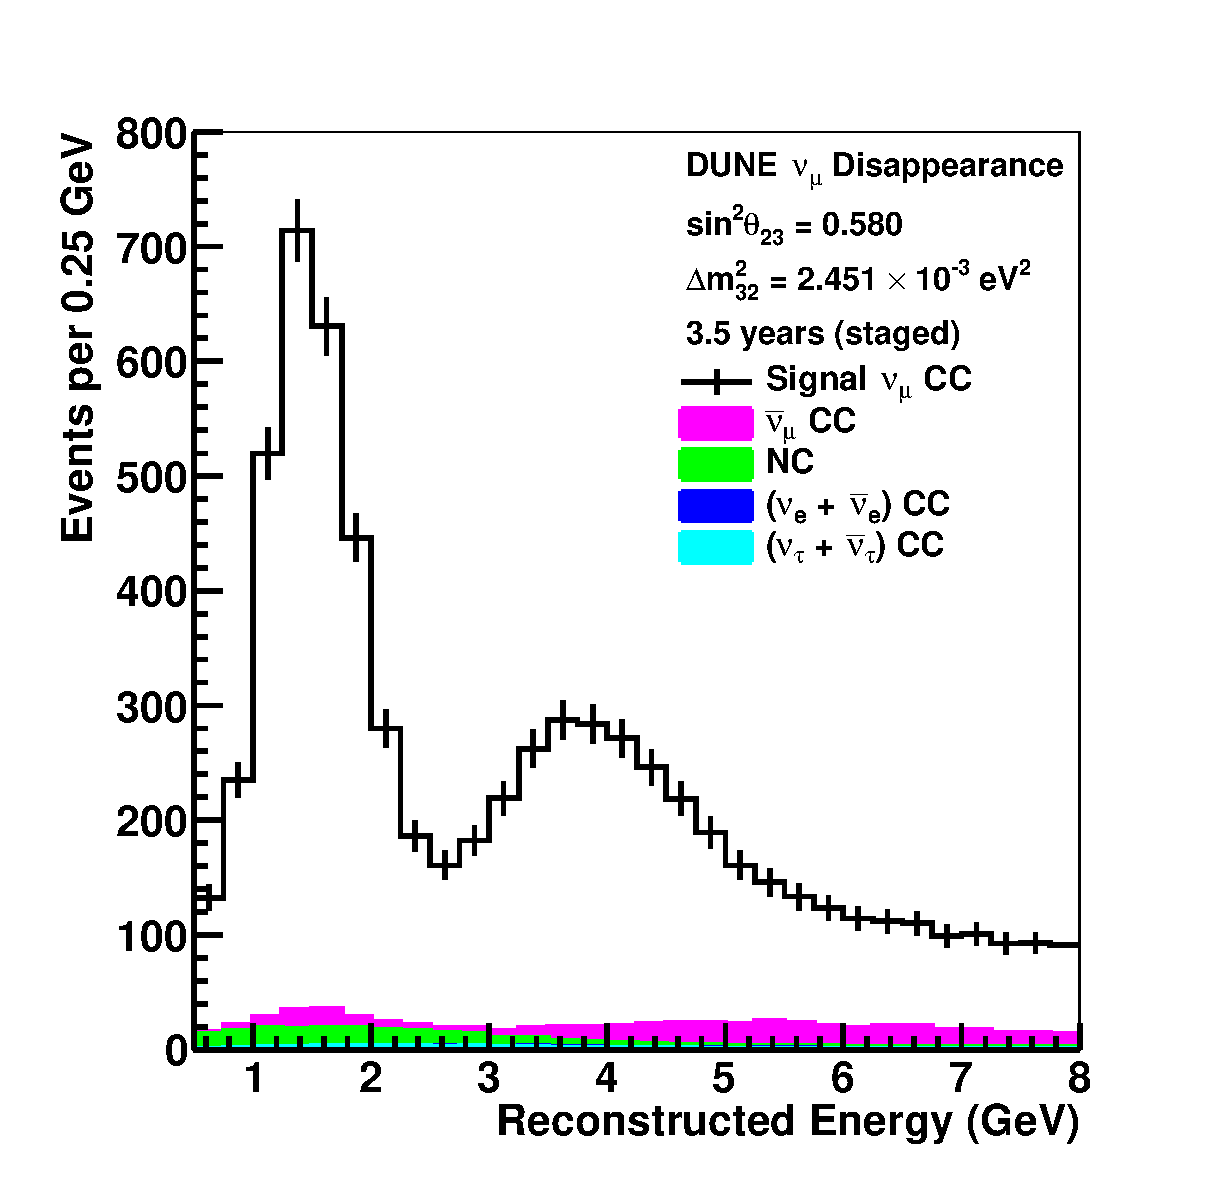
\includegraphics[width=\linewidth]{files/figures/dune_detector/spec_dis_nu_no}
    \caption{Disappearance events, neutrino mode}
  \end{subfigure}
  \hfill
  \begin{subfigure}[t]{.49\textwidth}
    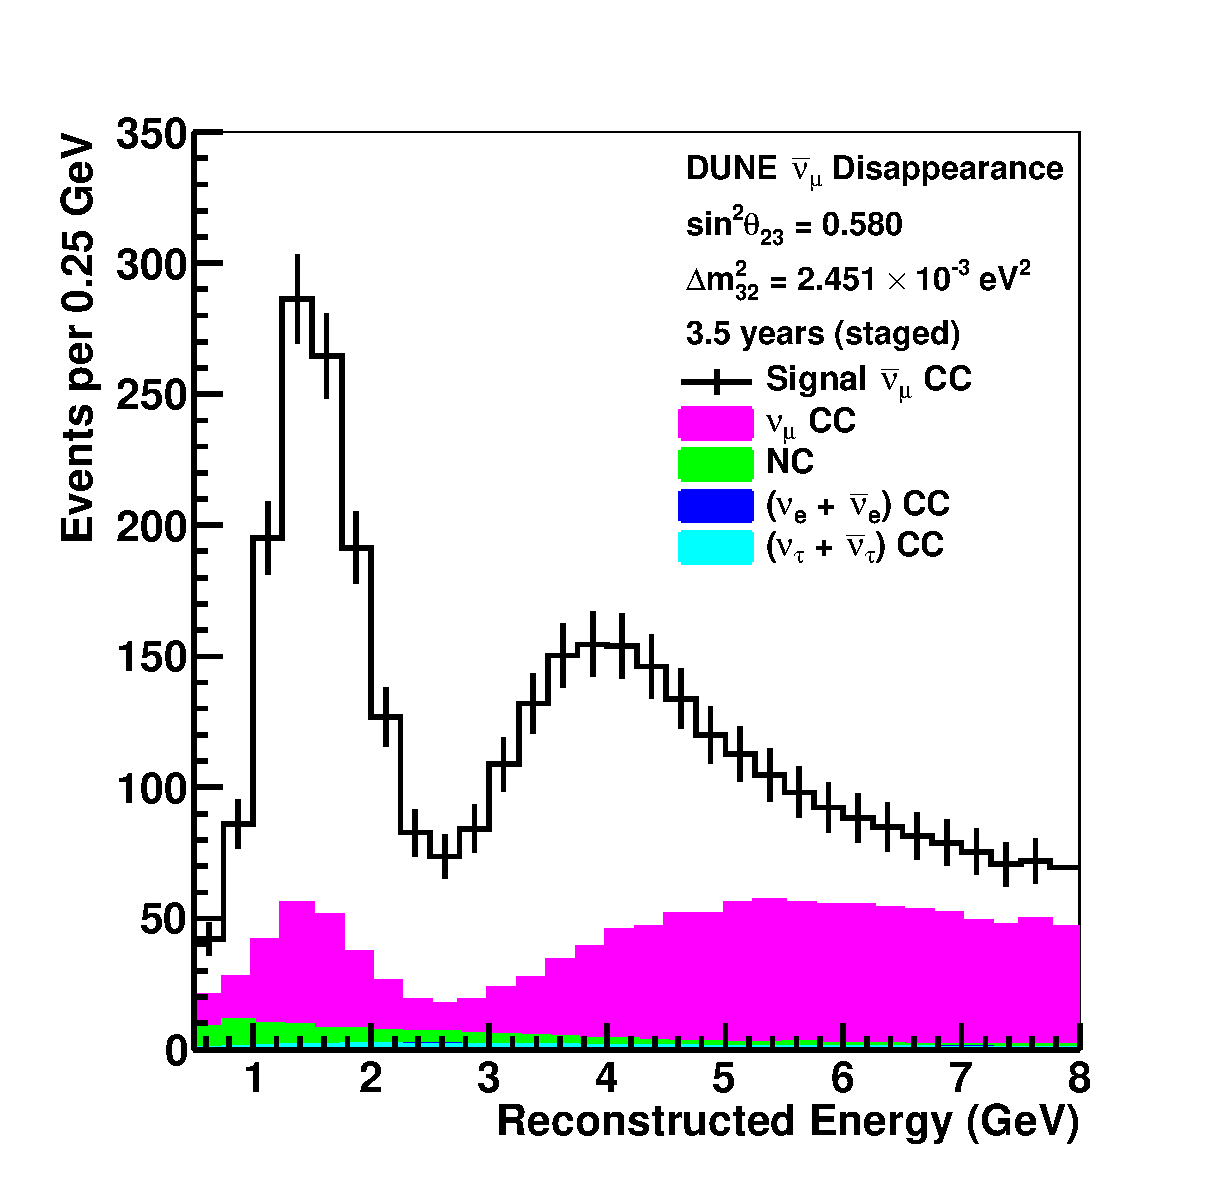
\includegraphics[width=\linewidth]{files/figures/dune_detector/spec_dis_anu_no}
    \caption{Disappearance events, antineutrino mode}
  \end{subfigure}
  \\
  \centering
  \begin{subfigure}[t]{.49\textwidth}
    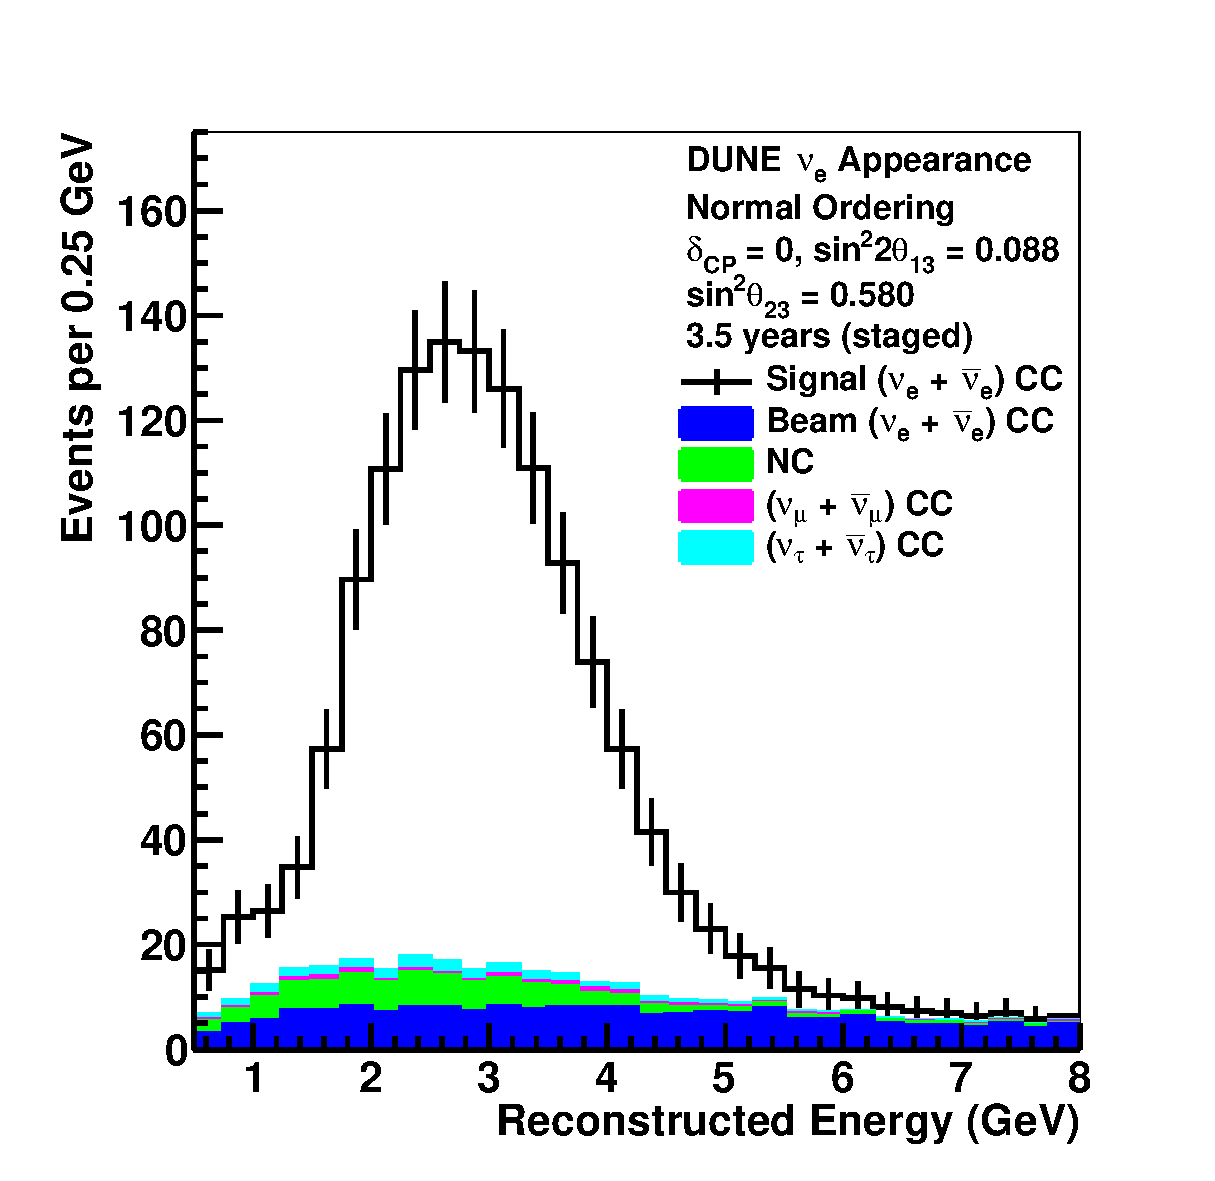
\includegraphics[width=\linewidth]{files/figures/dune_detector/spec_app_nu_no}
    \caption{Appearance events, neutrino mode}
  \end{subfigure}
  \hfill
  \begin{subfigure}[t]{.49\textwidth}
    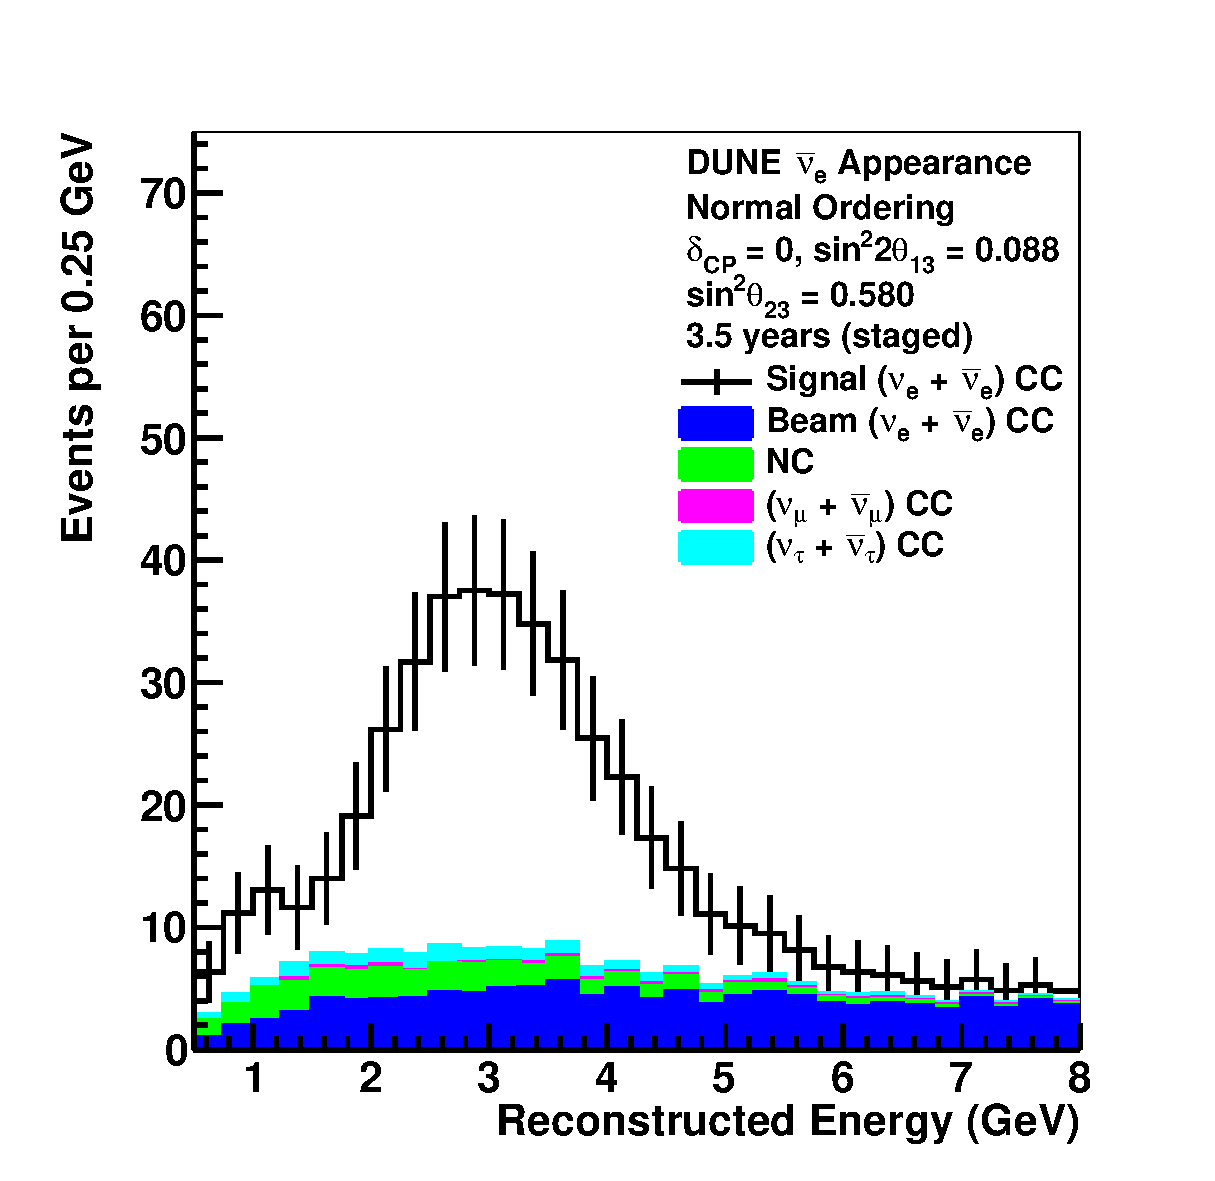
\includegraphics[width=\linewidth]{files/figures/dune_detector/spec_app_anu_no}
    \caption{Appearance events, antineutrino mode}
  \end{subfigure}
  \caption[DUNE far detector event rates.]{DUNE far detector event rates for appearance and disappearance channels in neutrino and antineutrino mode, from~\cite{tdrVol2}. For each of the subplots, the oscillation parameters are set to the best fit points from~\cite{nufit4} apart from \dcp which is set to 0. For all sub-plots, the mass hierarchy is normal.}
  \label{fig:fdEventRates}
\end{figure}

The far detector will consist of four liquid argon time projection chambers (LArTPCs).
At least two of the far detector modules will use single-phase LArTPC technology while alternative options including dual-phase LArTPCs are being explored for the other modules.
These modules will combine excellent particle identification and energy resolution with a large, monolithic detector mass. 
The operational principles of LArTPCs will be discussed further in \citesec{sec:dune:fd:lartpc}.

Secondly, DUNE will use a neutrino beam with a wide spread of neutrino energies which, given the values of the mass splittings, will allow it to cover both the first and second oscillation maxima.
Measuring multiple oscillation maxima helps to reduce degeneracies between the measured oscillation parameters.
The need for this arises because, for a given neutrino energy, multiple sets of parameter values can realise the same oscillation probability.

Some of the benefits of the broad band beam are shown in \citefig{fig:nueRates}.
\citefig{fig:nueRates} is a `bi-rate' plot which shows the rates of \nue and \anue interactions at the far detector for various values of the oscillation parameters.
To make each of the ellipses, all oscillation parameters are held constant other than \dcp which is varied.
The blue (green) ellipses show the rates for the first (second) oscillation maximum.
The first oscillation maximum is defined as neutrino energies higher than the approximate first oscillation minimum at \SI{1.3}{\giga\electronvolt}, while the second oscillation maximum is defined as anything below this.
The solid (dashed) lines show the rates for the normal (inverted) neutrino mass hierarchy.
The red and black points highlight the maximally CP-violating cases.
Here, $\thetai{23}=\pi/4$ while the other mixing angles and mass splittings are at their best fit points according to Ref.~\cite{nufit4}.

\begin{figure}[h]
  \begin{minipage}[t]{0.5\textwidth}
    \begin{adjustbox}{max totalsize={\textwidth}, center}
      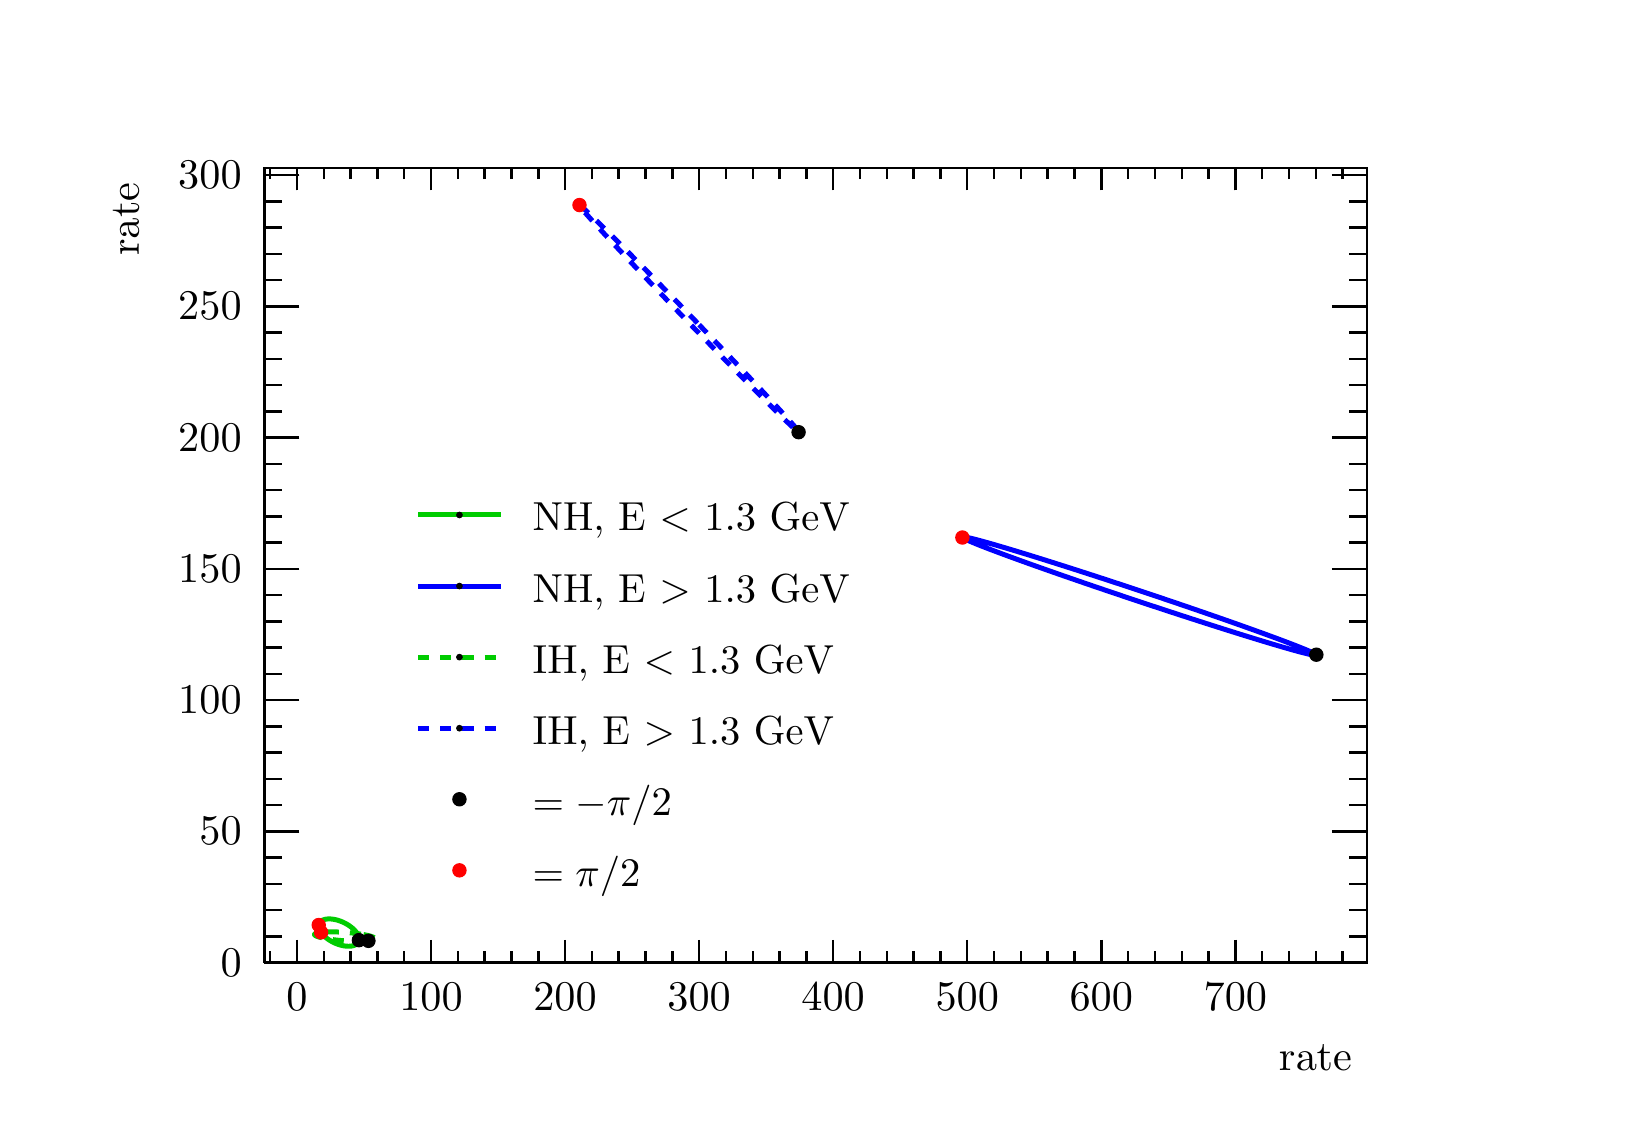
\begin{tikzpicture}
\pgfdeclareplotmark{cross} {
\pgfpathmoveto{\pgfpoint{-0.3\pgfplotmarksize}{\pgfplotmarksize}}
\pgfpathlineto{\pgfpoint{+0.3\pgfplotmarksize}{\pgfplotmarksize}}
\pgfpathlineto{\pgfpoint{+0.3\pgfplotmarksize}{0.3\pgfplotmarksize}}
\pgfpathlineto{\pgfpoint{+1\pgfplotmarksize}{0.3\pgfplotmarksize}}
\pgfpathlineto{\pgfpoint{+1\pgfplotmarksize}{-0.3\pgfplotmarksize}}
\pgfpathlineto{\pgfpoint{+0.3\pgfplotmarksize}{-0.3\pgfplotmarksize}}
\pgfpathlineto{\pgfpoint{+0.3\pgfplotmarksize}{-1.\pgfplotmarksize}}
\pgfpathlineto{\pgfpoint{-0.3\pgfplotmarksize}{-1.\pgfplotmarksize}}
\pgfpathlineto{\pgfpoint{-0.3\pgfplotmarksize}{-0.3\pgfplotmarksize}}
\pgfpathlineto{\pgfpoint{-1.\pgfplotmarksize}{-0.3\pgfplotmarksize}}
\pgfpathlineto{\pgfpoint{-1.\pgfplotmarksize}{0.3\pgfplotmarksize}}
\pgfpathlineto{\pgfpoint{-0.3\pgfplotmarksize}{0.3\pgfplotmarksize}}
\pgfpathclose
\pgfusepathqstroke
}
\pgfdeclareplotmark{cross*} {
\pgfpathmoveto{\pgfpoint{-0.3\pgfplotmarksize}{\pgfplotmarksize}}
\pgfpathlineto{\pgfpoint{+0.3\pgfplotmarksize}{\pgfplotmarksize}}
\pgfpathlineto{\pgfpoint{+0.3\pgfplotmarksize}{0.3\pgfplotmarksize}}
\pgfpathlineto{\pgfpoint{+1\pgfplotmarksize}{0.3\pgfplotmarksize}}
\pgfpathlineto{\pgfpoint{+1\pgfplotmarksize}{-0.3\pgfplotmarksize}}
\pgfpathlineto{\pgfpoint{+0.3\pgfplotmarksize}{-0.3\pgfplotmarksize}}
\pgfpathlineto{\pgfpoint{+0.3\pgfplotmarksize}{-1.\pgfplotmarksize}}
\pgfpathlineto{\pgfpoint{-0.3\pgfplotmarksize}{-1.\pgfplotmarksize}}
\pgfpathlineto{\pgfpoint{-0.3\pgfplotmarksize}{-0.3\pgfplotmarksize}}
\pgfpathlineto{\pgfpoint{-1.\pgfplotmarksize}{-0.3\pgfplotmarksize}}
\pgfpathlineto{\pgfpoint{-1.\pgfplotmarksize}{0.3\pgfplotmarksize}}
\pgfpathlineto{\pgfpoint{-0.3\pgfplotmarksize}{0.3\pgfplotmarksize}}
\pgfpathclose
\pgfusepathqfillstroke
}
\pgfdeclareplotmark{newstar} {
\pgfpathmoveto{\pgfqpoint{0pt}{\pgfplotmarksize}}
\pgfpathlineto{\pgfqpointpolar{44}{0.5\pgfplotmarksize}}
\pgfpathlineto{\pgfqpointpolar{18}{\pgfplotmarksize}}
\pgfpathlineto{\pgfqpointpolar{-20}{0.5\pgfplotmarksize}}
\pgfpathlineto{\pgfqpointpolar{-54}{\pgfplotmarksize}}
\pgfpathlineto{\pgfqpointpolar{-90}{0.5\pgfplotmarksize}}
\pgfpathlineto{\pgfqpointpolar{234}{\pgfplotmarksize}}
\pgfpathlineto{\pgfqpointpolar{198}{0.5\pgfplotmarksize}}
\pgfpathlineto{\pgfqpointpolar{162}{\pgfplotmarksize}}
\pgfpathlineto{\pgfqpointpolar{134}{0.5\pgfplotmarksize}}
\pgfpathclose
\pgfusepathqstroke
}
\pgfdeclareplotmark{newstar*} {
\pgfpathmoveto{\pgfqpoint{0pt}{\pgfplotmarksize}}
\pgfpathlineto{\pgfqpointpolar{44}{0.5\pgfplotmarksize}}
\pgfpathlineto{\pgfqpointpolar{18}{\pgfplotmarksize}}
\pgfpathlineto{\pgfqpointpolar{-20}{0.5\pgfplotmarksize}}
\pgfpathlineto{\pgfqpointpolar{-54}{\pgfplotmarksize}}
\pgfpathlineto{\pgfqpointpolar{-90}{0.5\pgfplotmarksize}}
\pgfpathlineto{\pgfqpointpolar{234}{\pgfplotmarksize}}
\pgfpathlineto{\pgfqpointpolar{198}{0.5\pgfplotmarksize}}
\pgfpathlineto{\pgfqpointpolar{162}{\pgfplotmarksize}}
\pgfpathlineto{\pgfqpointpolar{134}{0.5\pgfplotmarksize}}
\pgfpathclose
\pgfusepathqfillstroke
}
\definecolor{c}{rgb}{1,1,1};
\draw [color=c, fill=c] (0,0) rectangle (20,13.639);
\draw [color=c, fill=c] (3,1.77307) rectangle (17,11.8659);
\definecolor{c}{rgb}{0,0,0};
\draw [c,line width=0.9] (3,1.77307) -- (3,11.8659) -- (17,11.8659) -- (17,1.77307) -- (3,1.77307);
\definecolor{c}{rgb}{1,1,1};
\draw [color=c, fill=c] (3,1.77307) rectangle (17,11.8659);
\definecolor{c}{rgb}{0,0,0};
\draw [c,line width=0.9] (3,1.77307) -- (3,11.8659) -- (17,11.8659) -- (17,1.77307) -- (3,1.77307);
\draw [c,line width=0.9] (3,1.77307) -- (17,1.77307);
\draw [c,line width=0.9] (3.41282,2.05948) -- (3.41282,1.77307);
\draw [c,line width=0.9] (3.75333,1.91628) -- (3.75333,1.77307);
\draw [c,line width=0.9] (4.09383,1.91628) -- (4.09383,1.77307);
\draw [c,line width=0.9] (4.43433,1.91628) -- (4.43433,1.77307);
\draw [c,line width=0.9] (4.77484,1.91628) -- (4.77484,1.77307);
\draw [c,line width=0.9] (5.11534,2.05948) -- (5.11534,1.77307);
\draw [c,line width=0.9] (5.45585,1.91628) -- (5.45585,1.77307);
\draw [c,line width=0.9] (5.79635,1.91628) -- (5.79635,1.77307);
\draw [c,line width=0.9] (6.13686,1.91628) -- (6.13686,1.77307);
\draw [c,line width=0.9] (6.47736,1.91628) -- (6.47736,1.77307);
\draw [c,line width=0.9] (6.81786,2.05948) -- (6.81786,1.77307);
\draw [c,line width=0.9] (7.15837,1.91628) -- (7.15837,1.77307);
\draw [c,line width=0.9] (7.49887,1.91628) -- (7.49887,1.77307);
\draw [c,line width=0.9] (7.83938,1.91628) -- (7.83938,1.77307);
\draw [c,line width=0.9] (8.17988,1.91628) -- (8.17988,1.77307);
\draw [c,line width=0.9] (8.52039,2.05948) -- (8.52039,1.77307);
\draw [c,line width=0.9] (8.86089,1.91628) -- (8.86089,1.77307);
\draw [c,line width=0.9] (9.20139,1.91628) -- (9.20139,1.77307);
\draw [c,line width=0.9] (9.5419,1.91628) -- (9.5419,1.77307);
\draw [c,line width=0.9] (9.8824,1.91628) -- (9.8824,1.77307);
\draw [c,line width=0.9] (10.2229,2.05948) -- (10.2229,1.77307);
\draw [c,line width=0.9] (10.5634,1.91628) -- (10.5634,1.77307);
\draw [c,line width=0.9] (10.9039,1.91628) -- (10.9039,1.77307);
\draw [c,line width=0.9] (11.2444,1.91628) -- (11.2444,1.77307);
\draw [c,line width=0.9] (11.5849,1.91628) -- (11.5849,1.77307);
\draw [c,line width=0.9] (11.9254,2.05948) -- (11.9254,1.77307);
\draw [c,line width=0.9] (12.2659,1.91628) -- (12.2659,1.77307);
\draw [c,line width=0.9] (12.6064,1.91628) -- (12.6064,1.77307);
\draw [c,line width=0.9] (12.9469,1.91628) -- (12.9469,1.77307);
\draw [c,line width=0.9] (13.2874,1.91628) -- (13.2874,1.77307);
\draw [c,line width=0.9] (13.628,2.05948) -- (13.628,1.77307);
\draw [c,line width=0.9] (13.9685,1.91628) -- (13.9685,1.77307);
\draw [c,line width=0.9] (14.309,1.91628) -- (14.309,1.77307);
\draw [c,line width=0.9] (14.6495,1.91628) -- (14.6495,1.77307);
\draw [c,line width=0.9] (14.99,1.91628) -- (14.99,1.77307);
\draw [c,line width=0.9] (15.3305,2.05948) -- (15.3305,1.77307);
\draw [c,line width=0.9] (3.41282,2.05948) -- (3.41282,1.77307);
\draw [c,line width=0.9] (3.07232,1.91628) -- (3.07232,1.77307);
\draw [c,line width=0.9] (15.3305,2.05948) -- (15.3305,1.77307);
\draw [c,line width=0.9] (15.671,1.91628) -- (15.671,1.77307);
\draw [c,line width=0.9] (16.0115,1.91628) -- (16.0115,1.77307);
\draw [c,line width=0.9] (16.352,1.91628) -- (16.352,1.77307);
\draw [c,line width=0.9] (16.6925,1.91628) -- (16.6925,1.77307);
\draw [anchor=base] (3.41282,1.15931) node[scale=1.52731, color=c, rotate=0]{0};
\draw [anchor=base] (5.11534,1.15931) node[scale=1.52731, color=c, rotate=0]{100};
\draw [anchor=base] (6.81786,1.15931) node[scale=1.52731, color=c, rotate=0]{200};
\draw [anchor=base] (8.52039,1.15931) node[scale=1.52731, color=c, rotate=0]{300};
\draw [anchor=base] (10.2229,1.15931) node[scale=1.52731, color=c, rotate=0]{400};
\draw [anchor=base] (11.9254,1.15931) node[scale=1.52731, color=c, rotate=0]{500};
\draw [anchor=base] (13.628,1.15931) node[scale=1.52731, color=c, rotate=0]{600};
\draw [anchor=base] (15.3305,1.15931) node[scale=1.52731, color=c, rotate=0]{700};
\draw [anchor= east] (17,0.572837) node[scale=1.52731, color=c, rotate=0]{\nue rate};
\draw [c,line width=0.9] (3,11.8659) -- (17,11.8659);
\draw [c,line width=0.9] (3.41282,11.5795) -- (3.41282,11.8659);
\draw [c,line width=0.9] (3.75333,11.7227) -- (3.75333,11.8659);
\draw [c,line width=0.9] (4.09383,11.7227) -- (4.09383,11.8659);
\draw [c,line width=0.9] (4.43433,11.7227) -- (4.43433,11.8659);
\draw [c,line width=0.9] (4.77484,11.7227) -- (4.77484,11.8659);
\draw [c,line width=0.9] (5.11534,11.5795) -- (5.11534,11.8659);
\draw [c,line width=0.9] (5.45585,11.7227) -- (5.45585,11.8659);
\draw [c,line width=0.9] (5.79635,11.7227) -- (5.79635,11.8659);
\draw [c,line width=0.9] (6.13686,11.7227) -- (6.13686,11.8659);
\draw [c,line width=0.9] (6.47736,11.7227) -- (6.47736,11.8659);
\draw [c,line width=0.9] (6.81786,11.5795) -- (6.81786,11.8659);
\draw [c,line width=0.9] (7.15837,11.7227) -- (7.15837,11.8659);
\draw [c,line width=0.9] (7.49887,11.7227) -- (7.49887,11.8659);
\draw [c,line width=0.9] (7.83938,11.7227) -- (7.83938,11.8659);
\draw [c,line width=0.9] (8.17988,11.7227) -- (8.17988,11.8659);
\draw [c,line width=0.9] (8.52039,11.5795) -- (8.52039,11.8659);
\draw [c,line width=0.9] (8.86089,11.7227) -- (8.86089,11.8659);
\draw [c,line width=0.9] (9.20139,11.7227) -- (9.20139,11.8659);
\draw [c,line width=0.9] (9.5419,11.7227) -- (9.5419,11.8659);
\draw [c,line width=0.9] (9.8824,11.7227) -- (9.8824,11.8659);
\draw [c,line width=0.9] (10.2229,11.5795) -- (10.2229,11.8659);
\draw [c,line width=0.9] (10.5634,11.7227) -- (10.5634,11.8659);
\draw [c,line width=0.9] (10.9039,11.7227) -- (10.9039,11.8659);
\draw [c,line width=0.9] (11.2444,11.7227) -- (11.2444,11.8659);
\draw [c,line width=0.9] (11.5849,11.7227) -- (11.5849,11.8659);
\draw [c,line width=0.9] (11.9254,11.5795) -- (11.9254,11.8659);
\draw [c,line width=0.9] (12.2659,11.7227) -- (12.2659,11.8659);
\draw [c,line width=0.9] (12.6064,11.7227) -- (12.6064,11.8659);
\draw [c,line width=0.9] (12.9469,11.7227) -- (12.9469,11.8659);
\draw [c,line width=0.9] (13.2874,11.7227) -- (13.2874,11.8659);
\draw [c,line width=0.9] (13.628,11.5795) -- (13.628,11.8659);
\draw [c,line width=0.9] (13.9685,11.7227) -- (13.9685,11.8659);
\draw [c,line width=0.9] (14.309,11.7227) -- (14.309,11.8659);
\draw [c,line width=0.9] (14.6495,11.7227) -- (14.6495,11.8659);
\draw [c,line width=0.9] (14.99,11.7227) -- (14.99,11.8659);
\draw [c,line width=0.9] (15.3305,11.5795) -- (15.3305,11.8659);
\draw [c,line width=0.9] (3.41282,11.5795) -- (3.41282,11.8659);
\draw [c,line width=0.9] (3.07232,11.7227) -- (3.07232,11.8659);
\draw [c,line width=0.9] (15.3305,11.5795) -- (15.3305,11.8659);
\draw [c,line width=0.9] (15.671,11.7227) -- (15.671,11.8659);
\draw [c,line width=0.9] (16.0115,11.7227) -- (16.0115,11.8659);
\draw [c,line width=0.9] (16.352,11.7227) -- (16.352,11.8659);
\draw [c,line width=0.9] (16.6925,11.7227) -- (16.6925,11.8659);
\draw [c,line width=0.9] (3,1.77307) -- (3,11.8659);
\draw [c,line width=0.9] (3.444,1.77307) -- (3,1.77307);
\draw [c,line width=0.9] (3.222,2.10645) -- (3,2.10645);
\draw [c,line width=0.9] (3.222,2.43983) -- (3,2.43983);
\draw [c,line width=0.9] (3.222,2.77321) -- (3,2.77321);
\draw [c,line width=0.9] (3.222,3.10659) -- (3,3.10659);
\draw [c,line width=0.9] (3.444,3.43997) -- (3,3.43997);
\draw [c,line width=0.9] (3.222,3.77335) -- (3,3.77335);
\draw [c,line width=0.9] (3.222,4.10674) -- (3,4.10674);
\draw [c,line width=0.9] (3.222,4.44012) -- (3,4.44012);
\draw [c,line width=0.9] (3.222,4.7735) -- (3,4.7735);
\draw [c,line width=0.9] (3.444,5.10688) -- (3,5.10688);
\draw [c,line width=0.9] (3.222,5.44026) -- (3,5.44026);
\draw [c,line width=0.9] (3.222,5.77364) -- (3,5.77364);
\draw [c,line width=0.9] (3.222,6.10702) -- (3,6.10702);
\draw [c,line width=0.9] (3.222,6.4404) -- (3,6.4404);
\draw [c,line width=0.9] (3.444,6.77379) -- (3,6.77379);
\draw [c,line width=0.9] (3.222,7.10717) -- (3,7.10717);
\draw [c,line width=0.9] (3.222,7.44055) -- (3,7.44055);
\draw [c,line width=0.9] (3.222,7.77393) -- (3,7.77393);
\draw [c,line width=0.9] (3.222,8.10731) -- (3,8.10731);
\draw [c,line width=0.9] (3.444,8.44069) -- (3,8.44069);
\draw [c,line width=0.9] (3.222,8.77407) -- (3,8.77407);
\draw [c,line width=0.9] (3.222,9.10746) -- (3,9.10746);
\draw [c,line width=0.9] (3.222,9.44084) -- (3,9.44084);
\draw [c,line width=0.9] (3.222,9.77422) -- (3,9.77422);
\draw [c,line width=0.9] (3.444,10.1076) -- (3,10.1076);
\draw [c,line width=0.9] (3.222,10.441) -- (3,10.441);
\draw [c,line width=0.9] (3.222,10.7744) -- (3,10.7744);
\draw [c,line width=0.9] (3.222,11.1077) -- (3,11.1077);
\draw [c,line width=0.9] (3.222,11.4411) -- (3,11.4411);
\draw [c,line width=0.9] (3.444,11.7745) -- (3,11.7745);
\draw [c,line width=0.9] (3.444,11.7745) -- (3,11.7745);
\draw [anchor= east] (2.9,1.77307) node[scale=1.52731, color=c, rotate=0]{0};
\draw [anchor= east] (2.9,3.43997) node[scale=1.52731, color=c, rotate=0]{50};
\draw [anchor= east] (2.9,5.10688) node[scale=1.52731, color=c, rotate=0]{100};
\draw [anchor= east] (2.9,6.77379) node[scale=1.52731, color=c, rotate=0]{150};
\draw [anchor= east] (2.9,8.44069) node[scale=1.52731, color=c, rotate=0]{200};
\draw [anchor= east] (2.9,10.1076) node[scale=1.52731, color=c, rotate=0]{250};
\draw [anchor= east] (2.9,11.7745) node[scale=1.52731, color=c, rotate=0]{300};
\draw [anchor= east] (1.24,11.8659) node[scale=1.52731, color=c, rotate=90]{\anue rate};
\draw [c,line width=0.9] (17,1.77307) -- (17,11.8659);
\draw [c,line width=0.9] (16.556,1.77307) -- (17,1.77307);
\draw [c,line width=0.9] (16.778,2.10645) -- (17,2.10645);
\draw [c,line width=0.9] (16.778,2.43983) -- (17,2.43983);
\draw [c,line width=0.9] (16.778,2.77321) -- (17,2.77321);
\draw [c,line width=0.9] (16.778,3.10659) -- (17,3.10659);
\draw [c,line width=0.9] (16.556,3.43997) -- (17,3.43997);
\draw [c,line width=0.9] (16.778,3.77335) -- (17,3.77335);
\draw [c,line width=0.9] (16.778,4.10674) -- (17,4.10674);
\draw [c,line width=0.9] (16.778,4.44012) -- (17,4.44012);
\draw [c,line width=0.9] (16.778,4.7735) -- (17,4.7735);
\draw [c,line width=0.9] (16.556,5.10688) -- (17,5.10688);
\draw [c,line width=0.9] (16.778,5.44026) -- (17,5.44026);
\draw [c,line width=0.9] (16.778,5.77364) -- (17,5.77364);
\draw [c,line width=0.9] (16.778,6.10702) -- (17,6.10702);
\draw [c,line width=0.9] (16.778,6.4404) -- (17,6.4404);
\draw [c,line width=0.9] (16.556,6.77379) -- (17,6.77379);
\draw [c,line width=0.9] (16.778,7.10717) -- (17,7.10717);
\draw [c,line width=0.9] (16.778,7.44055) -- (17,7.44055);
\draw [c,line width=0.9] (16.778,7.77393) -- (17,7.77393);
\draw [c,line width=0.9] (16.778,8.10731) -- (17,8.10731);
\draw [c,line width=0.9] (16.556,8.44069) -- (17,8.44069);
\draw [c,line width=0.9] (16.778,8.77407) -- (17,8.77407);
\draw [c,line width=0.9] (16.778,9.10746) -- (17,9.10746);
\draw [c,line width=0.9] (16.778,9.44084) -- (17,9.44084);
\draw [c,line width=0.9] (16.778,9.77422) -- (17,9.77422);
\draw [c,line width=0.9] (16.556,10.1076) -- (17,10.1076);
\draw [c,line width=0.9] (16.778,10.441) -- (17,10.441);
\draw [c,line width=0.9] (16.778,10.7744) -- (17,10.7744);
\draw [c,line width=0.9] (16.778,11.1077) -- (17,11.1077);
\draw [c,line width=0.9] (16.778,11.4411) -- (17,11.4411);
\draw [c,line width=0.9] (16.556,11.7745) -- (17,11.7745);
\draw [c,line width=0.9] (16.556,11.7745) -- (17,11.7745);
\definecolor{c}{rgb}{0,0.8,0};
\draw [c,line width=1.8] (3.92242,2.00908) -- (3.93044,2.00613) -- (3.93848,2.00333) -- (3.94652,2.00067) -- (3.95456,1.99817) -- (3.96259,1.99582) -- (3.9706,1.99363) -- (3.97859,1.99159) -- (3.98654,1.98971) -- (3.99446,1.988) -- (4.00232,1.98645)
 -- (4.01012,1.98506) -- (4.01786,1.98384) -- (4.02553,1.98279) -- (4.03312,1.9819) -- (4.04062,1.98119) -- (4.04803,1.98064) -- (4.05533,1.98027) -- (4.06252,1.98006) -- (4.0696,1.98003) -- (4.07656,1.98017) -- (4.08338,1.98048) -- (4.09007,1.98097)
 -- (4.09661,1.98162) -- (4.103,1.98244) -- (4.10924,1.98343) -- (4.11532,1.98459) -- (4.12122,1.98591) -- (4.12695,1.98741) -- (4.13251,1.98906) -- (4.13787,1.99088) -- (4.14305,1.99286) -- (4.14803,1.99499) -- (4.1528,1.99729) -- (4.15738,1.99973)
 -- (4.16174,2.00233) -- (4.16589,2.00508) -- (4.16982,2.00798) -- (4.17353,2.01102) -- (4.17701,2.0142) -- (4.18026,2.01751) -- (4.18328,2.02096) -- (4.18606,2.02455) -- (4.18861,2.02826) -- (4.19091,2.03209) -- (4.19298,2.03604) --
 (4.19479,2.04011) -- (4.19636,2.0443) -- (4.19768,2.04858) -- (4.19875,2.05298) -- (4.19957,2.05747) -- (4.20014,2.06206) -- (4.20046,2.06674) -- (4.20052,2.0715) -- (4.20033,2.07634) -- (4.19989,2.08126) -- (4.1992,2.08626) -- (4.19825,2.09131) --
 (4.19706,2.09643) -- (4.19561,2.10161) -- (4.19392,2.10684) -- (4.19198,2.11211) -- (4.1898,2.11743) -- (4.18737,2.12278) -- (4.18471,2.12816) -- (4.18181,2.13356) -- (4.17867,2.13899) -- (4.17531,2.14443) -- (4.17171,2.14988) -- (4.16789,2.15533)
 -- (4.16386,2.16079) -- (4.1596,2.16623) -- (4.15513,2.17166) -- (4.15046,2.17708) -- (4.14558,2.18247) -- (4.1405,2.18783) -- (4.13523,2.19316) -- (4.12977,2.19845) -- (4.12413,2.20369) -- (4.11831,2.20889) -- (4.11232,2.21403) -- (4.10616,2.21911)
 -- (4.09985,2.22413) -- (4.09338,2.22908) -- (4.08676,2.23395) -- (4.08001,2.23874) -- (4.07312,2.24345) -- (4.0661,2.24807) -- (4.05897,2.2526) -- (4.05172,2.25703) -- (4.04436,2.26136) -- (4.03691,2.26558) -- (4.02936,2.26969) -- (4.02173,2.27369)
 -- (4.01403,2.27757) -- (4.00625,2.28132) -- (3.99842,2.28495) -- (3.99053,2.28845) -- (3.9826,2.29182) -- (3.97463,2.29505) -- (3.96663,2.29814) -- (3.95861,2.30109) -- (3.95057,2.3039) -- (3.94253,2.30655) -- (3.93449,2.30905) -- (3.92646,2.3114)
 -- (3.91845,2.3136) -- (3.91046,2.31564) -- (3.90251,2.31751) -- (3.89459,2.31923) -- (3.88673,2.32078) -- (3.87893,2.32217) -- (3.87119,2.32339) -- (3.86352,2.32444) -- (3.85593,2.32532) -- (3.84843,2.32604) -- (3.84102,2.32658) --
 (3.83372,2.32696) -- (3.82653,2.32716) -- (3.81945,2.32719) -- (3.81249,2.32705) -- (3.80567,2.32674) -- (3.79898,2.32626) -- (3.79244,2.32561) -- (3.78605,2.32478) -- (3.77981,2.32379) -- (3.77373,2.32264) -- (3.76783,2.32131) -- (3.7621,2.31982)
 -- (3.75655,2.31816) -- (3.75118,2.31635) -- (3.746,2.31437) -- (3.74102,2.31223) -- (3.73625,2.30994) -- (3.73167,2.30749) -- (3.72731,2.30489) -- (3.72316,2.30214) -- (3.71923,2.29925) -- (3.71552,2.29621) -- (3.71204,2.29303) -- (3.70879,2.28971)
 -- (3.70577,2.28626) -- (3.70299,2.28268) -- (3.70044,2.27897) -- (3.69814,2.27513) -- (3.69608,2.27118) -- (3.69426,2.26711) -- (3.69269,2.26293) -- (3.69137,2.25864) -- (3.6903,2.25425) -- (3.68948,2.24975) -- (3.68891,2.24517) --
 (3.68859,2.24049) -- (3.68853,2.23573) -- (3.68872,2.23088) -- (3.68916,2.22596) -- (3.68985,2.22097) -- (3.6908,2.21591) -- (3.69199,2.21079) -- (3.69344,2.20561) -- (3.69513,2.20039) -- (3.69707,2.19511) -- (3.69925,2.1898) -- (3.70168,2.18445) --
 (3.70434,2.17907) -- (3.70724,2.17366) -- (3.71038,2.16823) -- (3.71374,2.16279) -- (3.71734,2.15734) -- (3.72116,2.15189) -- (3.7252,2.14644) -- (3.72945,2.141) -- (3.73392,2.13556) -- (3.73859,2.13015) -- (3.74347,2.12476) -- (3.74855,2.1194) --
 (3.75382,2.11407) -- (3.75928,2.10878) -- (3.76492,2.10353) -- (3.77074,2.09834) -- (3.77673,2.09319) -- (3.78289,2.08811) -- (3.7892,2.0831) -- (3.79567,2.07815) -- (3.80229,2.07328) -- (3.80904,2.06848) -- (3.81593,2.06377) -- (3.82295,2.05915) --
 (3.83009,2.05462) -- (3.83733,2.05019) -- (3.84469,2.04586) -- (3.85214,2.04164) -- (3.85969,2.03753) -- (3.86732,2.03353) -- (3.87502,2.02966) -- (3.8828,2.0259) -- (3.89063,2.02227) -- (3.89852,2.01877) -- (3.90645,2.0154) -- (3.91442,2.01217) --
 (3.92242,2.00908);
\definecolor{c}{rgb}{0,0,1};
\draw [c,line width=1.8] (14.256,6.30899) -- (14.3265,6.28567) -- (14.3969,6.26249) -- (14.4669,6.23948) -- (14.5366,6.21665) -- (14.6058,6.19402) -- (14.6746,6.17163) -- (14.7428,6.14949) -- (14.8104,6.12762) -- (14.8773,6.10605) --
 (14.9435,6.08479) -- (15.0088,6.06387) -- (15.0732,6.04331) -- (15.1367,6.02313) -- (15.1992,6.00335) -- (15.2606,5.98398) -- (15.3209,5.96505) -- (15.38,5.94658) -- (15.4378,5.92858) -- (15.4943,5.91107) -- (15.5495,5.89407) -- (15.6032,5.8776) --
 (15.6555,5.86167) -- (15.7062,5.8463) -- (15.7554,5.8315) -- (15.8029,5.81728) -- (15.8488,5.80367) -- (15.893,5.79067) -- (15.9354,5.77831) -- (15.976,5.76658) -- (16.0147,5.7555) -- (16.0516,5.74508) -- (16.0866,5.73534) -- (16.1196,5.72628) --
 (16.1506,5.71791) -- (16.1797,5.71025) -- (16.2066,5.70328) -- (16.2316,5.69704) -- (16.2544,5.69151) -- (16.2751,5.68671) -- (16.2937,5.68263) -- (16.3101,5.6793) -- (16.3243,5.6767) -- (16.3364,5.67484) -- (16.3463,5.67372) -- (16.3539,5.67335) --
 (16.3594,5.67372) -- (16.3626,5.67483) -- (16.3636,5.67668) -- (16.3624,5.67928) -- (16.359,5.68261) -- (16.3533,5.68668) -- (16.3455,5.69147) -- (16.3354,5.697) -- (16.3231,5.70324) -- (16.3087,5.7102) -- (16.2921,5.71786) -- (16.2733,5.72623) --
 (16.2524,5.73528) -- (16.2294,5.74502) -- (16.2043,5.75543) -- (16.1771,5.7665) -- (16.1479,5.77823) -- (16.1167,5.79059) -- (16.0835,5.80359) -- (16.0484,5.81719) -- (16.0113,5.8314) -- (15.9724,5.8462) -- (15.9316,5.86157) -- (15.8891,5.8775) --
 (15.8448,5.89397) -- (15.7987,5.91096) -- (15.751,5.92847) -- (15.7017,5.94646) -- (15.6509,5.96493) -- (15.5985,5.98386) -- (15.5446,6.00322) -- (15.4893,6.023) -- (15.4327,6.04318) -- (15.3747,6.06374) -- (15.3155,6.08466) -- (15.2552,6.10591) --
 (15.1936,6.12748) -- (15.1311,6.14935) -- (15.0675,6.17149) -- (15.003,6.19388) -- (14.9376,6.2165) -- (14.8713,6.23933) -- (14.8044,6.26234) -- (14.7367,6.28552) -- (14.6684,6.30884) -- (14.5996,6.33227) -- (14.5303,6.35579) -- (14.4606,6.37939) --
 (14.3905,6.40303) -- (14.3202,6.4267) -- (14.2497,6.45036) -- (14.179,6.47401) -- (14.1082,6.4976) -- (14.0375,6.52113) -- (13.9668,6.54456) -- (13.8963,6.56788) -- (13.826,6.59105) -- (13.756,6.61407) -- (13.6863,6.6369) -- (13.617,6.65952) --
 (13.5482,6.68192) -- (13.48,6.70406) -- (13.4124,6.72593) -- (13.3455,6.7475) -- (13.2794,6.76875) -- (13.214,6.78967) -- (13.1496,6.81023) -- (13.0861,6.83042) -- (13.0236,6.8502) -- (12.9622,6.86957) -- (12.9019,6.88849) -- (12.8429,6.90697) --
 (12.785,6.92497) -- (12.7285,6.94247) -- (12.6734,6.95947) -- (12.6196,6.97595) -- (12.5674,6.99188) -- (12.5166,7.00725) -- (12.4674,7.02205) -- (12.4199,7.03626) -- (12.374,7.04988) -- (12.3299,7.06287) -- (12.2875,7.07524) -- (12.2469,7.08697) --
 (12.2081,7.09805) -- (12.1712,7.10846) -- (12.1363,7.1182) -- (12.1032,7.12726) -- (12.0722,7.13563) -- (12.0432,7.1433) -- (12.0162,7.15026) -- (11.9913,7.15651) -- (11.9685,7.16204) -- (11.9477,7.16684) -- (11.9292,7.17091) -- (11.9127,7.17425) --
 (11.8985,7.17685) -- (11.8864,7.17871) -- (11.8766,7.17983) -- (11.8689,7.1802) -- (11.8634,7.17983) -- (11.8602,7.17872) -- (11.8592,7.17686) -- (11.8604,7.17427) -- (11.8638,7.17094) -- (11.8695,7.16687) -- (11.8774,7.16207) -- (11.8874,7.15655)
 -- (11.8997,7.15031) -- (11.9141,7.14335) -- (11.9308,7.13568) -- (11.9495,7.12732) -- (11.9704,7.11827) -- (11.9934,7.10853) -- (12.0185,7.09812) -- (12.0457,7.08704) -- (12.0749,7.07532) -- (12.1061,7.06295) -- (12.1393,7.04996) --
 (12.1745,7.03635) -- (12.2115,7.02214) -- (12.2504,7.00735) -- (12.2912,6.99198) -- (12.3338,6.97605) -- (12.3781,6.95958) -- (12.4241,6.94259) -- (12.4718,6.92508) -- (12.5211,6.90709) -- (12.572,6.88862) -- (12.6244,6.86969) -- (12.6783,6.85033)
 -- (12.7335,6.83054) -- (12.7902,6.81037) -- (12.8481,6.78981) -- (12.9073,6.76889) -- (12.9677,6.74764) -- (13.0292,6.72607) -- (13.0918,6.7042) -- (13.1553,6.68206) -- (13.2199,6.65967) -- (13.2853,6.63705) -- (13.3515,6.61422) -- (13.4185,6.5912)
 -- (13.4861,6.56803) -- (13.5544,6.54471) -- (13.6232,6.52128) -- (13.6925,6.49775) -- (13.7622,6.47416) -- (13.8323,6.45052) -- (13.9026,6.42685) -- (13.9732,6.40318) -- (14.0439,6.37954) -- (14.1146,6.35595) -- (14.1853,6.33242) --
 (14.256,6.30899);
\definecolor{c}{rgb}{0,0.8,0};
\draw [c,dash pattern=on 4.00pt off 4.00pt ,line width=1.8] (4.25881,2.12821) -- (4.26812,2.1265) -- (4.27719,2.12476) -- (4.28601,2.12301) -- (4.29457,2.12123) -- (4.30285,2.11943) -- (4.31086,2.11762) -- (4.31857,2.1158) -- (4.326,2.11396) --
 (4.33312,2.11211) -- (4.33993,2.11025) -- (4.34643,2.10838) -- (4.3526,2.10651) -- (4.35845,2.10463) -- (4.36396,2.10276) -- (4.36914,2.10088) -- (4.37396,2.099) -- (4.37844,2.09713) -- (4.38257,2.09527) -- (4.38634,2.09341) -- (4.38974,2.09156) --
 (4.39278,2.08972) -- (4.39546,2.08789) -- (4.39776,2.08608) -- (4.39969,2.08429) -- (4.40125,2.08251) -- (4.40243,2.08076) -- (4.40323,2.07902) -- (4.40365,2.07731) -- (4.4037,2.07562) -- (4.40336,2.07397) -- (4.40265,2.07234) -- (4.40156,2.07073)
 -- (4.4001,2.06917) -- (4.39826,2.06763) -- (4.39604,2.06613) -- (4.39346,2.06467) -- (4.3905,2.06324) -- (4.38718,2.06185) -- (4.3835,2.0605) -- (4.37946,2.0592) -- (4.37507,2.05793) -- (4.37032,2.05672) -- (4.36523,2.05554) -- (4.3598,2.05442) --
 (4.35403,2.05334) -- (4.34793,2.05231) -- (4.34151,2.05133) -- (4.33478,2.0504) -- (4.32773,2.04952) -- (4.32038,2.0487) -- (4.31273,2.04792) -- (4.30479,2.04721) -- (4.29657,2.04654) -- (4.28808,2.04594) -- (4.27933,2.04539) -- (4.27031,2.04489) --
 (4.26106,2.04446) -- (4.25156,2.04408) -- (4.24183,2.04375) -- (4.23189,2.04349) -- (4.22174,2.04329) -- (4.21139,2.04314) -- (4.20084,2.04305) -- (4.19013,2.04303) -- (4.17924,2.04306) -- (4.16819,2.04315) -- (4.157,2.04329) -- (4.14568,2.0435) --
 (4.13423,2.04377) -- (4.12267,2.04409) -- (4.111,2.04447) -- (4.09925,2.04491) -- (4.08742,2.04541) -- (4.07552,2.04596) -- (4.06357,2.04657) -- (4.05157,2.04724) -- (4.03954,2.04796) -- (4.0275,2.04873) -- (4.01544,2.04956) -- (4.0034,2.05044) --
 (3.99136,2.05137) -- (3.97936,2.05235) -- (3.96739,2.05339) -- (3.95548,2.05447) -- (3.94363,2.05559) -- (3.93186,2.05677) -- (3.92017,2.05799) -- (3.90859,2.05925) -- (3.89711,2.06056) -- (3.88575,2.06191) -- (3.87453,2.0633) -- (3.86345,2.06473)
 -- (3.85252,2.0662) -- (3.84176,2.0677) -- (3.83118,2.06924) -- (3.82078,2.07081) -- (3.81058,2.07241) -- (3.80058,2.07404) -- (3.79081,2.0757) -- (3.78125,2.07739) -- (3.77194,2.0791) -- (3.76287,2.08083) -- (3.75405,2.08259) -- (3.74549,2.08437)
 -- (3.73721,2.08616) -- (3.7292,2.08798) -- (3.72149,2.0898) -- (3.71406,2.09164) -- (3.70694,2.09349) -- (3.70013,2.09535) -- (3.69363,2.09722) -- (3.68746,2.09909) -- (3.68161,2.10096) -- (3.6761,2.10284) -- (3.67093,2.10472) -- (3.6661,2.10659)
 -- (3.66162,2.10847) -- (3.65749,2.11033) -- (3.65372,2.11219) -- (3.65032,2.11404) -- (3.64728,2.11588) -- (3.6446,2.11771) -- (3.6423,2.11952) -- (3.64037,2.12131) -- (3.63881,2.12309) -- (3.63763,2.12484) -- (3.63683,2.12658) -- (3.63641,2.12829)
 -- (3.63636,2.12997) -- (3.6367,2.13163) -- (3.63741,2.13326) -- (3.6385,2.13486) -- (3.63996,2.13643) -- (3.6418,2.13797) -- (3.64402,2.13947) -- (3.6466,2.14093) -- (3.64956,2.14236) -- (3.65288,2.14375) -- (3.65656,2.1451) -- (3.6606,2.1464) --
 (3.66499,2.14766) -- (3.66974,2.14888) -- (3.67483,2.15006) -- (3.68026,2.15118) -- (3.68603,2.15226) -- (3.69213,2.15329) -- (3.69855,2.15427) -- (3.70528,2.1552) -- (3.71233,2.15608) -- (3.71968,2.1569) -- (3.72733,2.15767) -- (3.73527,2.15839) --
 (3.74349,2.15905) -- (3.75198,2.15966) -- (3.76074,2.16021) -- (3.76975,2.16071) -- (3.77901,2.16114) -- (3.7885,2.16152) -- (3.79823,2.16184) -- (3.80817,2.16211) -- (3.81832,2.16231) -- (3.82868,2.16246) -- (3.83922,2.16254) -- (3.84994,2.16257)
 -- (3.86082,2.16254) -- (3.87187,2.16245) -- (3.88306,2.1623) -- (3.89438,2.1621) -- (3.90583,2.16183) -- (3.91739,2.16151) -- (3.92906,2.16112) -- (3.94081,2.16068) -- (3.95264,2.16019) -- (3.96454,2.15963) -- (3.97649,2.15902) -- (3.98849,2.15836)
 -- (4.00052,2.15764) -- (4.01256,2.15687) -- (4.02462,2.15604) -- (4.03667,2.15516) -- (4.0487,2.15423) -- (4.0607,2.15324) -- (4.07267,2.15221) -- (4.08458,2.15113) -- (4.09643,2.15) -- (4.1082,2.14883) -- (4.11989,2.14761) -- (4.13147,2.14634) --
 (4.14295,2.14504) -- (4.15431,2.14369) -- (4.16553,2.1423) -- (4.17661,2.14087) -- (4.18754,2.1394) -- (4.1983,2.1379) -- (4.20888,2.13636) -- (4.21928,2.13479) -- (4.22948,2.13319) -- (4.23948,2.13156) -- (4.24925,2.1299) -- (4.25881,2.12821);
\definecolor{c}{rgb}{0,0,1};
\draw [c,dash pattern=on 4.00pt off 4.00pt ,line width=1.8] (8.52006,9.87307) -- (8.56369,9.82781) -- (8.60716,9.78266) -- (8.65042,9.73768) -- (8.69342,9.69292) -- (8.73612,9.6484) -- (8.77849,9.60419) -- (8.82047,9.56032) -- (8.86203,9.51683) --
 (8.90312,9.47377) -- (8.94372,9.43118) -- (8.98377,9.3891) -- (9.02323,9.34758) -- (9.06207,9.30666) -- (9.10025,9.26637) -- (9.13773,9.22675) -- (9.17448,9.18785) -- (9.21045,9.14971) -- (9.24562,9.11235) -- (9.27995,9.07582) -- (9.31339,9.04015)
 -- (9.34593,9.00539) -- (9.37753,8.97155) -- (9.40816,8.93869) -- (9.43778,8.90682) -- (9.46637,8.87598) -- (9.4939,8.8462) -- (9.52035,8.81751) -- (9.54568,8.78994) -- (9.56987,8.76352) -- (9.5929,8.73827) -- (9.61475,8.71421) -- (9.63539,8.69138)
 -- (9.6548,8.66979) -- (9.67297,8.64946) -- (9.68987,8.63042) -- (9.70549,8.61268) -- (9.71981,8.59626) -- (9.73283,8.58117) -- (9.74452,8.56744) -- (9.75488,8.55508) -- (9.76389,8.54409) -- (9.77155,8.53449) -- (9.77785,8.52629) --
 (9.78278,8.51949) -- (9.78634,8.5141) -- (9.78852,8.51014) -- (9.78933,8.50759) -- (9.78875,8.50647) -- (9.7868,8.50678) -- (9.78347,8.50851) -- (9.77877,8.51166) -- (9.7727,8.51624) -- (9.76527,8.52223) -- (9.75648,8.52962) -- (9.74635,8.53843) --
 (9.73488,8.54862) -- (9.72209,8.5602) -- (9.70798,8.57315) -- (9.69257,8.58747) -- (9.67588,8.60312) -- (9.65793,8.62011) -- (9.63872,8.63841) -- (9.61829,8.658) -- (9.59664,8.67888) -- (9.57381,8.701) -- (9.54981,8.72436) -- (9.52467,8.74893) --
 (9.49841,8.77469) -- (9.47106,8.80161) -- (9.44264,8.82966) -- (9.41319,8.85882) -- (9.38273,8.88905) -- (9.35129,8.92033) -- (9.31891,8.95263) -- (9.28561,8.98592) -- (9.25143,9.02016) -- (9.2164,9.05531) -- (9.18056,9.09135) -- (9.14394,9.12824)
 -- (9.10658,9.16594) -- (9.06851,9.20441) -- (9.02978,9.24362) -- (8.99041,9.28353) -- (8.95046,9.3241) -- (8.90996,9.36528) -- (8.86894,9.40705) -- (8.82746,9.44935) -- (8.78554,9.49214) -- (8.74324,9.53539) -- (8.70059,9.57905) --
 (8.65764,9.62307) -- (8.61442,9.66742) -- (8.57098,9.71205) -- (8.52737,9.75691) -- (8.48363,9.80197) -- (8.43979,9.84717) -- (8.39591,9.89247) -- (8.35203,9.93783) -- (8.30818,9.98321) -- (8.26442,10.0285) -- (8.22078,10.0738) -- (8.17731,10.119)
 -- (8.13406,10.1639) -- (8.09106,10.2087) -- (8.04835,10.2532) -- (8.00599,10.2974) -- (7.96401,10.3413) -- (7.92245,10.3848) -- (7.88135,10.4279) -- (7.84076,10.4704) -- (7.80071,10.5125) -- (7.76125,10.554) -- (7.7224,10.595) -- (7.68422,10.6353)
 -- (7.64674,10.6749) -- (7.61,10.7138) -- (7.57402,10.7519) -- (7.53885,10.7893) -- (7.50453,10.8258) -- (7.47108,10.8615) -- (7.43854,10.8962) -- (7.40694,10.9301) -- (7.37632,10.9629) -- (7.34669,10.9948) -- (7.3181,11.0256) -- (7.29057,11.0554)
 -- (7.26413,11.0841) -- (7.2388,11.1117) -- (7.2146,11.1381) -- (7.19157,11.1634) -- (7.16973,11.1874) -- (7.14909,11.2102) -- (7.12968,11.2318) -- (7.11151,11.2522) -- (7.09461,11.2712) -- (7.07899,11.2889) -- (7.06466,11.3054) -- (7.05165,11.3204)
 -- (7.03995,11.3342) -- (7.02959,11.3465) -- (7.02058,11.3575) -- (7.01292,11.3671) -- (7.00662,11.3753) -- (7.00169,11.3821) -- (6.99813,11.3875) -- (6.99595,11.3915) -- (6.99515,11.394) -- (6.99572,11.3951) -- (6.99767,11.3948) -- (7.001,11.3931)
 -- (7.0057,11.39) -- (7.01177,11.3854) -- (7.0192,11.3794) -- (7.02799,11.372) -- (7.03813,11.3632) -- (7.04959,11.353) -- (7.06239,11.3414) -- (7.0765,11.3285) -- (7.0919,11.3142) -- (7.10859,11.2985) -- (7.12655,11.2815) -- (7.14575,11.2632) --
 (7.16619,11.2436) -- (7.18783,11.2227) -- (7.21067,11.2006) -- (7.23467,11.1773) -- (7.25981,11.1527) -- (7.28607,11.1269) -- (7.31342,11.1) -- (7.34183,11.072) -- (7.37129,11.0428) -- (7.40175,11.0126) -- (7.43318,10.9813) -- (7.46557,10.949) --
 (7.49887,10.9157) -- (7.53305,10.8815) -- (7.56808,10.8463) -- (7.60392,10.8103) -- (7.64054,10.7734) -- (7.6779,10.7357) -- (7.71596,10.6972) -- (7.7547,10.658) -- (7.79406,10.6181) -- (7.83401,10.5775) -- (7.87452,10.5363) -- (7.91553,10.4946) --
 (7.95702,10.4523) -- (7.99893,10.4095) -- (8.04124,10.3662) -- (8.08389,10.3226) -- (8.12684,10.2785) -- (8.17006,10.2342) -- (8.21349,10.1896) -- (8.2571,10.1447) -- (8.30085,10.0997) -- (8.34468,10.0545) -- (8.38856,10.0091) -- (8.43245,9.96379)
 -- (8.47629,9.91841) -- (8.52006,9.87307);
\definecolor{c}{rgb}{1,1,1};
\draw [color=c, fill=c] (2,12.8206) rectangle (18,13.5708);
\definecolor{c}{rgb}{0,0,0};
%\draw (10,13.1957) node[scale=1.40004, color=c, rotate=0]{$Comparison of \nu_{e} rates at the DUNE far detector$};
\foreach \P in {(4.19957,2.05747)}{\draw[mark options={color=c,fill=c},mark size=2.402402pt,mark=*] plot coordinates {\P};}
\definecolor{c}{rgb}{1,0,0};
\foreach \P in {(3.68948,2.24975)}{\draw[mark options={color=c,fill=c},mark size=2.402402pt,mark=*] plot coordinates {\P};}
\foreach \P in {(3.71968,2.1569)}{\draw[mark options={color=c,fill=c},mark size=2.402402pt,mark=*] plot coordinates {\P};}
\definecolor{c}{rgb}{0,0,0};
\foreach \P in {(4.32038,2.0487)}{\draw[mark options={color=c,fill=c},mark size=2.402402pt,mark=*] plot coordinates {\P};}
\foreach \P in {(9.78347,8.50851)}{\draw[mark options={color=c,fill=c},mark size=2.402402pt,mark=*] plot coordinates {\P};}
\definecolor{c}{rgb}{1,0,0};
\foreach \P in {(7.001,11.3931)}{\draw[mark options={color=c,fill=c},mark size=2.402402pt,mark=*] plot coordinates {\P};}
\foreach \P in {(11.8638,7.17094)}{\draw[mark options={color=c,fill=c},mark size=2.402402pt,mark=*] plot coordinates {\P};}
\definecolor{c}{rgb}{0,0,0};
\foreach \P in {(16.359,5.68261)}{\draw[mark options={color=c,fill=c},mark size=2.402402pt,mark=*] plot coordinates {\P};}
\definecolor{c}{rgb}{1,1,1};
\draw [color=c, fill=c] (4.72779,2.49284) rectangle (10.7163,7.90831);
\definecolor{c}{rgb}{0,0,0};
\draw [anchor=base west] (6.22493,7.25394) node[scale=1.46368, color=c, rotate=0]{NH, E $<$ 1.3 GeV};
\definecolor{c}{rgb}{1,1,1};
\draw [c, fill=c] (4.95236,7.14112) -- (6.00036,7.14112) -- (6.00036,7.77292) -- (4.95236,7.77292);
\definecolor{c}{rgb}{0,0.8,0};
\draw [c,line width=1.8] (4.95236,7.45702) -- (6.00036,7.45702);
\definecolor{c}{rgb}{0,0,0};
\foreach \P in {(5.47636,7.45702)}{\draw[mark options={color=c,fill=c},mark size=2.402402pt,mark=*,mark size=1pt] plot coordinates {\P};}
\draw [anchor=base west] (6.22493,6.35136) node[scale=1.46368, color=c, rotate=0]{NH, E $>$ 1.3 GeV};
\definecolor{c}{rgb}{1,1,1};
\draw [c, fill=c] (4.95236,6.23854) -- (6.00036,6.23854) -- (6.00036,6.87034) -- (4.95236,6.87034);
\definecolor{c}{rgb}{0,0,1};
\draw [c,line width=1.8] (4.95236,6.55444) -- (6.00036,6.55444);
\definecolor{c}{rgb}{0,0,0};
\foreach \P in {(5.47636,6.55444)}{\draw[mark options={color=c,fill=c},mark size=2.402402pt,mark=*,mark size=1pt] plot coordinates {\P};}
\draw [anchor=base west] (6.22493,5.44878) node[scale=1.46368, color=c, rotate=0]{IH, E $<$ 1.3 GeV};
\definecolor{c}{rgb}{1,1,1};
\draw [c, fill=c] (4.95236,5.33596) -- (6.00036,5.33596) -- (6.00036,5.96776) -- (4.95236,5.96776);
\definecolor{c}{rgb}{0,0.8,0};
\draw [c,dash pattern=on 4.00pt off 4.00pt ,line width=1.8] (4.95236,5.65186) -- (6.00036,5.65186);
\definecolor{c}{rgb}{0,0,0};
\foreach \P in {(5.47636,5.65186)}{\draw[mark options={color=c,fill=c},mark size=2.402402pt,mark=*,mark size=1pt] plot coordinates {\P};}
\draw [anchor=base west] (6.22493,4.5462) node[scale=1.46368, color=c, rotate=0]{IH, E $>$ 1.3 GeV};
\definecolor{c}{rgb}{1,1,1};
\draw [c, fill=c] (4.95236,4.43338) -- (6.00036,4.43338) -- (6.00036,5.06519) -- (4.95236,5.06519);
\definecolor{c}{rgb}{0,0,1};
\draw [c,dash pattern=on 4.00pt off 4.00pt ,line width=1.8] (4.95236,4.74928) -- (6.00036,4.74928);
\definecolor{c}{rgb}{0,0,0};
\foreach \P in {(5.47636,4.74928)}{\draw[mark options={color=c,fill=c},mark size=2.402402pt,mark=*,mark size=1pt] plot coordinates {\P};}
\draw [anchor=base west] (6.22493,3.64362) node[scale=1.46368, color=c, rotate=0]{$\dcp=-\pi/2$};
\foreach \P in {(5.47636,3.8467)}{\draw[mark options={color=c,fill=c},mark size=2.402402pt,mark=*] plot coordinates {\P};}
\draw [anchor=base west] (6.22493,2.74105) node[scale=1.46368, color=c, rotate=0]{$\dcp=\pi/2$};
\definecolor{c}{rgb}{1,0,0};
\foreach \P in {(5.47636,2.94413)}{\draw[mark options={color=c,fill=c},mark size=2.402402pt,mark=*] plot coordinates {\P};}
\end{tikzpicture}

    \end{adjustbox}
  \end{minipage}
  \hfill
  \begin{minipage}[t]{0.5\textwidth}
    \begin{adjustbox}{max totalsize={\textwidth}, center}
      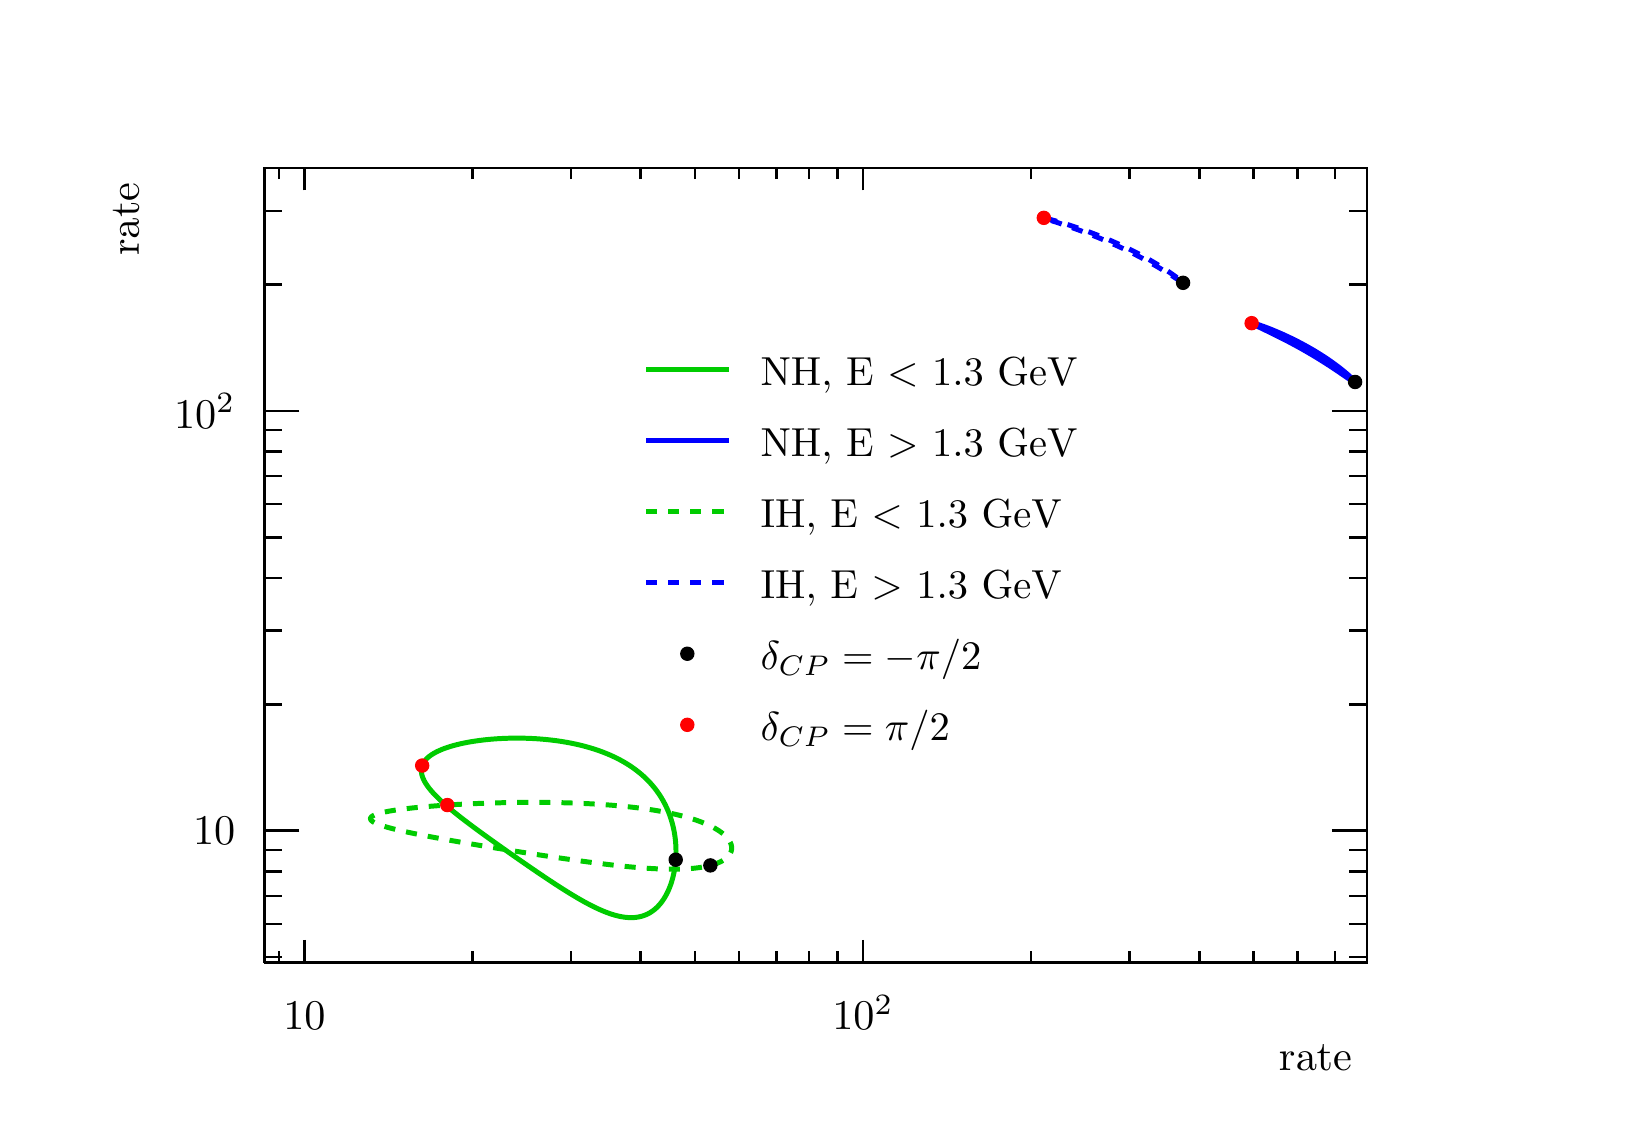
\begin{tikzpicture}
\pgfdeclareplotmark{cross} {
\pgfpathmoveto{\pgfpoint{-0.3\pgfplotmarksize}{\pgfplotmarksize}}
\pgfpathlineto{\pgfpoint{+0.3\pgfplotmarksize}{\pgfplotmarksize}}
\pgfpathlineto{\pgfpoint{+0.3\pgfplotmarksize}{0.3\pgfplotmarksize}}
\pgfpathlineto{\pgfpoint{+1\pgfplotmarksize}{0.3\pgfplotmarksize}}
\pgfpathlineto{\pgfpoint{+1\pgfplotmarksize}{-0.3\pgfplotmarksize}}
\pgfpathlineto{\pgfpoint{+0.3\pgfplotmarksize}{-0.3\pgfplotmarksize}}
\pgfpathlineto{\pgfpoint{+0.3\pgfplotmarksize}{-1.\pgfplotmarksize}}
\pgfpathlineto{\pgfpoint{-0.3\pgfplotmarksize}{-1.\pgfplotmarksize}}
\pgfpathlineto{\pgfpoint{-0.3\pgfplotmarksize}{-0.3\pgfplotmarksize}}
\pgfpathlineto{\pgfpoint{-1.\pgfplotmarksize}{-0.3\pgfplotmarksize}}
\pgfpathlineto{\pgfpoint{-1.\pgfplotmarksize}{0.3\pgfplotmarksize}}
\pgfpathlineto{\pgfpoint{-0.3\pgfplotmarksize}{0.3\pgfplotmarksize}}
\pgfpathclose
\pgfusepathqstroke
}
\pgfdeclareplotmark{cross*} {
\pgfpathmoveto{\pgfpoint{-0.3\pgfplotmarksize}{\pgfplotmarksize}}
\pgfpathlineto{\pgfpoint{+0.3\pgfplotmarksize}{\pgfplotmarksize}}
\pgfpathlineto{\pgfpoint{+0.3\pgfplotmarksize}{0.3\pgfplotmarksize}}
\pgfpathlineto{\pgfpoint{+1\pgfplotmarksize}{0.3\pgfplotmarksize}}
\pgfpathlineto{\pgfpoint{+1\pgfplotmarksize}{-0.3\pgfplotmarksize}}
\pgfpathlineto{\pgfpoint{+0.3\pgfplotmarksize}{-0.3\pgfplotmarksize}}
\pgfpathlineto{\pgfpoint{+0.3\pgfplotmarksize}{-1.\pgfplotmarksize}}
\pgfpathlineto{\pgfpoint{-0.3\pgfplotmarksize}{-1.\pgfplotmarksize}}
\pgfpathlineto{\pgfpoint{-0.3\pgfplotmarksize}{-0.3\pgfplotmarksize}}
\pgfpathlineto{\pgfpoint{-1.\pgfplotmarksize}{-0.3\pgfplotmarksize}}
\pgfpathlineto{\pgfpoint{-1.\pgfplotmarksize}{0.3\pgfplotmarksize}}
\pgfpathlineto{\pgfpoint{-0.3\pgfplotmarksize}{0.3\pgfplotmarksize}}
\pgfpathclose
\pgfusepathqfillstroke
}
\pgfdeclareplotmark{newstar} {
\pgfpathmoveto{\pgfqpoint{0pt}{\pgfplotmarksize}}
\pgfpathlineto{\pgfqpointpolar{44}{0.5\pgfplotmarksize}}
\pgfpathlineto{\pgfqpointpolar{18}{\pgfplotmarksize}}
\pgfpathlineto{\pgfqpointpolar{-20}{0.5\pgfplotmarksize}}
\pgfpathlineto{\pgfqpointpolar{-54}{\pgfplotmarksize}}
\pgfpathlineto{\pgfqpointpolar{-90}{0.5\pgfplotmarksize}}
\pgfpathlineto{\pgfqpointpolar{234}{\pgfplotmarksize}}
\pgfpathlineto{\pgfqpointpolar{198}{0.5\pgfplotmarksize}}
\pgfpathlineto{\pgfqpointpolar{162}{\pgfplotmarksize}}
\pgfpathlineto{\pgfqpointpolar{134}{0.5\pgfplotmarksize}}
\pgfpathclose
\pgfusepathqstroke
}
\pgfdeclareplotmark{newstar*} {
\pgfpathmoveto{\pgfqpoint{0pt}{\pgfplotmarksize}}
\pgfpathlineto{\pgfqpointpolar{44}{0.5\pgfplotmarksize}}
\pgfpathlineto{\pgfqpointpolar{18}{\pgfplotmarksize}}
\pgfpathlineto{\pgfqpointpolar{-20}{0.5\pgfplotmarksize}}
\pgfpathlineto{\pgfqpointpolar{-54}{\pgfplotmarksize}}
\pgfpathlineto{\pgfqpointpolar{-90}{0.5\pgfplotmarksize}}
\pgfpathlineto{\pgfqpointpolar{234}{\pgfplotmarksize}}
\pgfpathlineto{\pgfqpointpolar{198}{0.5\pgfplotmarksize}}
\pgfpathlineto{\pgfqpointpolar{162}{\pgfplotmarksize}}
\pgfpathlineto{\pgfqpointpolar{134}{0.5\pgfplotmarksize}}
\pgfpathclose
\pgfusepathqfillstroke
}
\definecolor{c}{rgb}{1,1,1};
\draw [color=c, fill=c] (0,0) rectangle (20,13.639);
\draw [color=c, fill=c] (3,1.77307) rectangle (17,11.8659);
\definecolor{c}{rgb}{0,0,0};
\draw [c,line width=0.9] (3,1.77307) -- (3,11.8659) -- (17,11.8659) -- (17,1.77307) -- (3,1.77307);
\definecolor{c}{rgb}{1,1,1};
\draw [color=c, fill=c] (3,1.77307) rectangle (17,11.8659);
\definecolor{c}{rgb}{0,0,0};
\draw [c,line width=0.9] (3,1.77307) -- (3,11.8659) -- (17,11.8659) -- (17,1.77307) -- (3,1.77307);
\draw [c,line width=0.9] (3,1.77307) -- (17,1.77307);
\draw [c,line width=0.9] (3.18294,1.91628) -- (3.18294,1.77307);
\draw [c,line width=0.9] (3.50753,2.05948) -- (3.50753,1.77307);
\draw [anchor=base] (3.50753,0.92063) node[scale=1.52731, color=c, rotate=0]{10};
\draw [c,line width=0.9] (5.64294,1.91628) -- (5.64294,1.77307);
\draw [c,line width=0.9] (6.89208,1.91628) -- (6.89208,1.77307);
\draw [c,line width=0.9] (7.77836,1.91628) -- (7.77836,1.77307);
\draw [c,line width=0.9] (8.46581,1.91628) -- (8.46581,1.77307);
\draw [c,line width=0.9] (9.0275,1.91628) -- (9.0275,1.77307);
\draw [c,line width=0.9] (9.5024,1.91628) -- (9.5024,1.77307);
\draw [c,line width=0.9] (9.91377,1.91628) -- (9.91377,1.77307);
\draw [c,line width=0.9] (10.2766,1.91628) -- (10.2766,1.77307);
\draw [c,line width=0.9] (10.6012,2.05948) -- (10.6012,1.77307);
\draw [anchor=base] (10.6012,0.92063) node[scale=1.52731, color=c, rotate=0]{$10^{2}$};
\draw [c,line width=0.9] (12.7366,1.91628) -- (12.7366,1.77307);
\draw [c,line width=0.9] (13.9858,1.91628) -- (13.9858,1.77307);
\draw [c,line width=0.9] (14.8721,1.91628) -- (14.8721,1.77307);
\draw [c,line width=0.9] (15.5595,1.91628) -- (15.5595,1.77307);
\draw [c,line width=0.9] (16.1212,1.91628) -- (16.1212,1.77307);
\draw [c,line width=0.9] (16.5961,1.91628) -- (16.5961,1.77307);
\draw [anchor= east] (17,0.572837) node[scale=1.52731, color=c, rotate=0]{\nue rate};
\draw [c,line width=0.9] (3,11.8659) -- (17,11.8659);
\draw [c,line width=0.9] (3.18294,11.7227) -- (3.18294,11.8659);
\draw [c,line width=0.9] (3.50753,11.5795) -- (3.50753,11.8659);
\draw [c,line width=0.9] (5.64294,11.7227) -- (5.64294,11.8659);
\draw [c,line width=0.9] (6.89208,11.7227) -- (6.89208,11.8659);
\draw [c,line width=0.9] (7.77836,11.7227) -- (7.77836,11.8659);
\draw [c,line width=0.9] (8.46581,11.7227) -- (8.46581,11.8659);
\draw [c,line width=0.9] (9.0275,11.7227) -- (9.0275,11.8659);
\draw [c,line width=0.9] (9.5024,11.7227) -- (9.5024,11.8659);
\draw [c,line width=0.9] (9.91377,11.7227) -- (9.91377,11.8659);
\draw [c,line width=0.9] (10.2766,11.7227) -- (10.2766,11.8659);
\draw [c,line width=0.9] (10.6012,11.5795) -- (10.6012,11.8659);
\draw [c,line width=0.9] (12.7366,11.7227) -- (12.7366,11.8659);
\draw [c,line width=0.9] (13.9858,11.7227) -- (13.9858,11.8659);
\draw [c,line width=0.9] (14.8721,11.7227) -- (14.8721,11.8659);
\draw [c,line width=0.9] (15.5595,11.7227) -- (15.5595,11.8659);
\draw [c,line width=0.9] (16.1212,11.7227) -- (16.1212,11.8659);
\draw [c,line width=0.9] (16.5961,11.7227) -- (16.5961,11.8659);
\draw [c,line width=0.9] (3,1.77307) -- (3,11.8659);
\draw [c,line width=0.9] (3.222,1.84242) -- (3,1.84242);
\draw [c,line width=0.9] (3.222,2.26449) -- (3,2.26449);
\draw [c,line width=0.9] (3.222,2.62135) -- (3,2.62135);
\draw [c,line width=0.9] (3.222,2.93047) -- (3,2.93047);
\draw [c,line width=0.9] (3.222,3.20314) -- (3,3.20314);
\draw [c,line width=0.9] (3.444,3.44704) -- (3,3.44704);
\draw [anchor= east] (2.82,3.44704) node[scale=1.52731, color=c, rotate=0]{10};
\draw [c,line width=0.9] (3.222,5.05166) -- (3,5.05166);
\draw [c,line width=0.9] (3.222,5.9903) -- (3,5.9903);
\draw [c,line width=0.9] (3.222,6.65628) -- (3,6.65628);
\draw [c,line width=0.9] (3.222,7.17285) -- (3,7.17285);
\draw [c,line width=0.9] (3.222,7.59492) -- (3,7.59492);
\draw [c,line width=0.9] (3.222,7.95178) -- (3,7.95178);
\draw [c,line width=0.9] (3.222,8.2609) -- (3,8.2609);
\draw [c,line width=0.9] (3.222,8.53357) -- (3,8.53357);
\draw [c,line width=0.9] (3.444,8.77747) -- (3,8.77747);
\draw [anchor= east] (2.82,8.77747) node[scale=1.52731, color=c, rotate=0]{$10^{2}$};
\draw [c,line width=0.9] (3.222,10.3821) -- (3,10.3821);
\draw [c,line width=0.9] (3.222,11.3207) -- (3,11.3207);
\draw [anchor= east] (1.24,11.8659) node[scale=1.52731, color=c, rotate=90]{\anue rate};
\draw [c,line width=0.9] (17,1.77307) -- (17,11.8659);
\draw [c,line width=0.9] (16.778,1.84242) -- (17,1.84242);
\draw [c,line width=0.9] (16.778,2.26449) -- (17,2.26449);
\draw [c,line width=0.9] (16.778,2.62135) -- (17,2.62135);
\draw [c,line width=0.9] (16.778,2.93047) -- (17,2.93047);
\draw [c,line width=0.9] (16.778,3.20314) -- (17,3.20314);
\draw [c,line width=0.9] (16.556,3.44704) -- (17,3.44704);
\draw [c,line width=0.9] (16.778,5.05166) -- (17,5.05166);
\draw [c,line width=0.9] (16.778,5.9903) -- (17,5.9903);
\draw [c,line width=0.9] (16.778,6.65628) -- (17,6.65628);
\draw [c,line width=0.9] (16.778,7.17285) -- (17,7.17285);
\draw [c,line width=0.9] (16.778,7.59492) -- (17,7.59492);
\draw [c,line width=0.9] (16.778,7.95178) -- (17,7.95178);
\draw [c,line width=0.9] (16.778,8.2609) -- (17,8.2609);
\draw [c,line width=0.9] (16.778,8.53357) -- (17,8.53357);
\draw [c,line width=0.9] (16.556,8.77747) -- (17,8.77747);
\draw [c,line width=0.9] (16.778,10.3821) -- (17,10.3821);
\draw [c,line width=0.9] (16.778,11.3207) -- (17,11.3207);
\definecolor{c}{rgb}{0,0.8,0};
\draw [c,line width=1.8] (6.88511,2.64748) -- (6.93323,2.61837) -- (6.98069,2.59036) -- (7.02747,2.56352) -- (7.07353,2.53791) -- (7.11886,2.51361) -- (7.16343,2.49069) -- (7.20723,2.46921) -- (7.25024,2.44924) -- (7.29243,2.43084) --
 (7.33379,2.41407) -- (7.37432,2.39898) -- (7.41398,2.38561) -- (7.45278,2.37402) -- (7.4907,2.36424) -- (7.52773,2.3563) -- (7.56386,2.35024) -- (7.59908,2.34606) -- (7.63339,2.34379) -- (7.66677,2.34344) -- (7.69922,2.345) -- (7.73073,2.34848) --
 (7.7613,2.35385) -- (7.79092,2.3611) -- (7.81959,2.3702) -- (7.84731,2.38113) -- (7.87406,2.39385) -- (7.89986,2.40831) -- (7.92468,2.42447) -- (7.94854,2.44228) -- (7.97142,2.46167) -- (7.99333,2.4826) -- (8.01427,2.505) -- (8.03423,2.5288) --
 (8.05321,2.55393) -- (8.07121,2.58032) -- (8.08822,2.60791) -- (8.10426,2.63662) -- (8.11931,2.66638) -- (8.13338,2.69711) -- (8.14646,2.72874) -- (8.15856,2.7612) -- (8.16967,2.79441) -- (8.1798,2.82832) -- (8.18894,2.86283) -- (8.19709,2.8979) --
 (8.20425,2.93345) -- (8.21043,2.96942) -- (8.21562,3.00574) -- (8.21982,3.04236) -- (8.22303,3.07922) -- (8.22526,3.11626) -- (8.22649,3.15343) -- (8.22674,3.19068) -- (8.226,3.22796) -- (8.22428,3.26522) -- (8.22156,3.30241) -- (8.21786,3.3395) --
 (8.21317,3.37645) -- (8.20749,3.41322) -- (8.20082,3.44976) -- (8.19316,3.48605) -- (8.18452,3.52206) -- (8.17489,3.55776) -- (8.16428,3.5931) -- (8.15268,3.62808) -- (8.14009,3.66267) -- (8.12652,3.69683) -- (8.11196,3.73055) -- (8.09642,3.76382)
 -- (8.0799,3.7966) -- (8.06239,3.82888) -- (8.0439,3.86064) -- (8.02444,3.89187) -- (8.00399,3.92256) -- (7.98257,3.95268) -- (7.96018,3.98224) -- (7.93681,4.0112) -- (7.91247,4.03957) -- (7.88717,4.06734) -- (7.8609,4.09449) -- (7.83366,4.12102) --
 (7.80547,4.14691) -- (7.77633,4.17216) -- (7.74624,4.19677) -- (7.7152,4.22073) -- (7.68322,4.24402) -- (7.6503,4.26665) -- (7.61646,4.28861) -- (7.5817,4.3099) -- (7.54603,4.33051) -- (7.50945,4.35044) -- (7.47198,4.36969) -- (7.43362,4.38824) --
 (7.39439,4.40611) -- (7.3543,4.42328) -- (7.31336,4.43975) -- (7.27158,4.45553) -- (7.22898,4.4706) -- (7.18558,4.48498) -- (7.14139,4.49865) -- (7.09644,4.51161) -- (7.05074,4.52387) -- (7.00432,4.53542) -- (6.9572,4.54625) -- (6.90941,4.55638) --
 (6.86098,4.5658) -- (6.81193,4.57451) -- (6.76229,4.5825) -- (6.71211,4.58978) -- (6.66142,4.59635) -- (6.61026,4.60221) -- (6.55867,4.60735) -- (6.5067,4.61177) -- (6.45439,4.61548) -- (6.40179,4.61847) -- (6.34897,4.62075) -- (6.29596,4.62232) --
 (6.24285,4.62316) -- (6.18969,4.6233) -- (6.13654,4.62271) -- (6.08349,4.62141) -- (6.03059,4.6194) -- (5.97794,4.61667) -- (5.92562,4.61322) -- (5.8737,4.60906) -- (5.82228,4.60418) -- (5.77145,4.59859) -- (5.7213,4.59229) -- (5.67194,4.58527) --
 (5.62347,4.57754) -- (5.57599,4.5691) -- (5.5296,4.55994) -- (5.48442,4.55007) -- (5.44055,4.53949) -- (5.3981,4.52821) -- (5.35719,4.51621) -- (5.31793,4.50351) -- (5.28043,4.4901) -- (5.24479,4.47599) -- (5.21112,4.46117) -- (5.17953,4.44565) --
 (5.15011,4.42943) -- (5.12296,4.41252) -- (5.09818,4.39491) -- (5.07584,4.37661) -- (5.05602,4.35762) -- (5.03879,4.33794) -- (5.02422,4.31758) -- (5.01235,4.29654) -- (5.00323,4.27483) -- (4.99689,4.25244) -- (4.99336,4.22939) -- (4.99265,4.20568)
 -- (4.99476,4.18131) -- (4.99969,4.15629) -- (5.00741,4.13064) -- (5.0179,4.10434) -- (5.03112,4.07742) -- (5.04702,4.04988) -- (5.06554,4.02173) -- (5.08662,3.99298) -- (5.11019,3.96365) -- (5.13615,3.93373) -- (5.16444,3.90325) --
 (5.19495,3.87222) -- (5.22758,3.84065) -- (5.26225,3.80856) -- (5.29882,3.77596) -- (5.33722,3.74287) -- (5.37731,3.70932) -- (5.419,3.67531) -- (5.46216,3.64088) -- (5.5067,3.60605) -- (5.55249,3.57083) -- (5.59944,3.53526) -- (5.64743,3.49937) --
 (5.69635,3.46317) -- (5.74611,3.42672) -- (5.79661,3.39003) -- (5.84775,3.35315) -- (5.89943,3.3161) -- (5.95156,3.27894) -- (6.00406,3.2417) -- (6.05684,3.20442) -- (6.10982,3.16716) -- (6.16293,3.12995) -- (6.21609,3.09286) -- (6.26924,3.05593) --
 (6.3223,3.01921) -- (6.37523,2.98277) -- (6.42794,2.94666) -- (6.4804,2.91095) -- (6.53255,2.8757) -- (6.58434,2.84097) -- (6.63573,2.80684) -- (6.68666,2.77336) -- (6.7371,2.74061) -- (6.78701,2.70867) -- (6.83636,2.6776) -- (6.88511,2.64748);
\definecolor{c}{rgb}{0,0,1};
\draw [c,line width=1.8] (16.305,9.49028) -- (16.325,9.47835) -- (16.3448,9.46643) -- (16.3644,9.45453) -- (16.3837,9.44267) -- (16.4028,9.43085) -- (16.4217,9.4191) -- (16.4403,9.40742) -- (16.4586,9.39582) -- (16.4767,9.38432) -- (16.4944,9.37294)
 -- (16.5118,9.36168) -- (16.5289,9.35056) -- (16.5456,9.33959) -- (16.562,9.32879) -- (16.578,9.31817) -- (16.5936,9.30774) -- (16.6089,9.29752) -- (16.6237,9.28751) -- (16.6382,9.27774) -- (16.6522,9.26821) -- (16.6658,9.25893) -- (16.679,9.24993)
 -- (16.6917,9.24121) -- (16.704,9.23278) -- (16.7159,9.22466) -- (16.7273,9.21686) -- (16.7382,9.20938) -- (16.7486,9.20224) -- (16.7586,9.19545) -- (16.7681,9.18902) -- (16.7771,9.18296) -- (16.7856,9.17728) -- (16.7936,9.17198) --
 (16.8011,9.16707) -- (16.8081,9.16257) -- (16.8146,9.15847) -- (16.8206,9.15479) -- (16.8261,9.15152) -- (16.8311,9.14869) -- (16.8355,9.14628) -- (16.8395,9.1443) -- (16.8429,9.14276) -- (16.8457,9.14165) -- (16.8481,9.14099) -- (16.8499,9.14077)
 -- (16.8512,9.14099) -- (16.852,9.14165) -- (16.8522,9.14275) -- (16.8519,9.14429) -- (16.8511,9.14626) -- (16.8498,9.14867) -- (16.8479,9.1515) -- (16.8455,9.15477) -- (16.8426,9.15845) -- (16.8391,9.16254) -- (16.8352,9.16704) -- (16.8307,9.17194)
 -- (16.8257,9.17724) -- (16.8201,9.18292) -- (16.8141,9.18898) -- (16.8075,9.19541) -- (16.8005,9.2022) -- (16.7929,9.20933) -- (16.7849,9.21681) -- (16.7763,9.22461) -- (16.7673,9.23273) -- (16.7577,9.24116) -- (16.7477,9.24988) --
 (16.7372,9.25888) -- (16.7262,9.26815) -- (16.7148,9.27767) -- (16.7029,9.28745) -- (16.6906,9.29745) -- (16.6778,9.30767) -- (16.6646,9.3181) -- (16.651,9.32872) -- (16.6369,9.33952) -- (16.6224,9.35049) -- (16.6075,9.36161) -- (16.5922,9.37286) --
 (16.5766,9.38425) -- (16.5605,9.39575) -- (16.5441,9.40734) -- (16.5274,9.41902) -- (16.5102,9.43078) -- (16.4928,9.44259) -- (16.4751,9.45446) -- (16.457,9.46636) -- (16.4387,9.47828) -- (16.42,9.49021) -- (16.4011,9.50214) -- (16.382,9.51405) --
 (16.3626,9.52594) -- (16.343,9.53779) -- (16.3232,9.54959) -- (16.3032,9.56134) -- (16.2831,9.57301) -- (16.2627,9.5846) -- (16.2423,9.5961) -- (16.2217,9.60749) -- (16.2011,9.61878) -- (16.1803,9.62994) -- (16.1596,9.64097) -- (16.1387,9.65187) --
 (16.1179,9.66261) -- (16.0971,9.67319) -- (16.0763,9.68361) -- (16.0555,9.69386) -- (16.0348,9.70392) -- (16.0142,9.71379) -- (15.9938,9.72346) -- (15.9734,9.73293) -- (15.9533,9.74219) -- (15.9333,9.75122) -- (15.9136,9.76004) -- (15.8941,9.76862)
 -- (15.8748,9.77697) -- (15.8559,9.78507) -- (15.8372,9.79292) -- (15.8189,9.80052) -- (15.801,9.80786) -- (15.7835,9.81494) -- (15.7664,9.82175) -- (15.7497,9.82829) -- (15.7335,9.83455) -- (15.7177,9.84052) -- (15.7025,9.84622) --
 (15.6878,9.85163) -- (15.6737,9.85674) -- (15.6601,9.86156) -- (15.6472,9.86609) -- (15.6349,9.87031) -- (15.6232,9.87423) -- (15.6122,9.87784) -- (15.6018,9.88115) -- (15.5922,9.88415) -- (15.5832,9.88684) -- (15.575,9.88922) -- (15.5676,9.89128)
 -- (15.5609,9.89302) -- (15.5549,9.89446) -- (15.5497,9.89557) -- (15.5454,9.89637) -- (15.5418,9.89684) -- (15.539,9.89701) -- (15.537,9.89685) -- (15.5358,9.89637) -- (15.5354,9.89558) -- (15.5359,9.89446) -- (15.5371,9.89303) -- (15.5392,9.89129)
 -- (15.5421,9.88923) -- (15.5457,9.88686) -- (15.5502,9.88417) -- (15.5554,9.88117) -- (15.5614,9.87787) -- (15.5682,9.87425) -- (15.5757,9.87033) -- (15.584,9.86611) -- (15.593,9.86159) -- (15.6027,9.85677) -- (15.6131,9.85166) -- (15.6242,9.84626)
 -- (15.636,9.84056) -- (15.6483,9.83459) -- (15.6613,9.82833) -- (15.6749,9.82179) -- (15.6891,9.81498) -- (15.7039,9.80791) -- (15.7191,9.80057) -- (15.7349,9.79297) -- (15.7512,9.78512) -- (15.7679,9.77702) -- (15.785,9.76867) -- (15.8026,9.76009)
 -- (15.8206,9.75128) -- (15.8389,9.74225) -- (15.8576,9.73299) -- (15.8765,9.72352) -- (15.8958,9.71385) -- (15.9153,9.70398) -- (15.9351,9.69392) -- (15.9551,9.68368) -- (15.9753,9.67326) -- (15.9956,9.66268) -- (16.0161,9.65194) --
 (16.0367,9.64105) -- (16.0574,9.63001) -- (16.0781,9.61885) -- (16.0989,9.60757) -- (16.1198,9.59617) -- (16.1406,9.58467) -- (16.1614,9.57308) -- (16.1822,9.56141) -- (16.2029,9.54967) -- (16.2236,9.53787) -- (16.2441,9.52602) -- (16.2646,9.51413)
 -- (16.2849,9.50221) -- (16.305,9.49028);
\definecolor{c}{rgb}{0,0.8,0};
\draw [c,dash pattern=on 4.00pt off 4.00pt ,line width=1.8] (8.44666,3.59344) -- (8.4804,3.58226) -- (8.51291,3.57086) -- (8.54417,3.55927) -- (8.57421,3.54748) -- (8.60302,3.53552) -- (8.63061,3.52338) -- (8.65697,3.51108) -- (8.68212,3.49862) --
 (8.70605,3.48602) -- (8.72877,3.47329) -- (8.75028,3.46044) -- (8.77059,3.44748) -- (8.7897,3.43442) -- (8.80761,3.42128) -- (8.82432,3.40805) -- (8.83983,3.39477) -- (8.85416,3.38144) -- (8.86729,3.36807) -- (8.87924,3.35467) -- (8.89,3.34127) --
 (8.89957,3.32787) -- (8.90797,3.31448) -- (8.91518,3.30113) -- (8.92121,3.28782) -- (8.92606,3.27457) -- (8.92974,3.26139) -- (8.93223,3.24831) -- (8.93355,3.23533) -- (8.93369,3.22247) -- (8.93266,3.20974) -- (8.93044,3.19716) -- (8.92705,3.18475)
 -- (8.92248,3.17252) -- (8.91673,3.16048) -- (8.9098,3.14865) -- (8.90169,3.13706) -- (8.8924,3.1257) -- (8.88192,3.1146) -- (8.87025,3.10377) -- (8.8574,3.09323) -- (8.84336,3.08299) -- (8.82813,3.07307) -- (8.81171,3.06348) -- (8.79409,3.05423) --
 (8.77527,3.04533) -- (8.75525,3.03681) -- (8.73402,3.02867) -- (8.71159,3.02093) -- (8.68795,3.01359) -- (8.66309,3.00668) -- (8.63702,3.00019) -- (8.60973,2.99414) -- (8.58121,2.98854) -- (8.55147,2.98339) -- (8.52049,2.97871) -- (8.48829,2.97451)
 -- (8.45484,2.97078) -- (8.42016,2.96755) -- (8.38423,2.9648) -- (8.34705,2.96254) -- (8.30863,2.96079) -- (8.26895,2.95954) -- (8.22801,2.95879) -- (8.18582,2.95855) -- (8.14236,2.95882) -- (8.09764,2.95959) -- (8.05166,2.96086) --
 (8.00442,2.96264) -- (7.95591,2.96491) -- (7.90613,2.96768) -- (7.85509,2.97094) -- (7.80278,2.97469) -- (7.74922,2.97892) -- (7.6944,2.98362) -- (7.63833,2.98878) -- (7.58101,2.9944) -- (7.52245,3.00047) -- (7.46265,3.00698) -- (7.40164,3.01392) --
 (7.33942,3.02127) -- (7.276,3.02903) -- (7.21141,3.03719) -- (7.14565,3.04573) -- (7.07876,3.05464) -- (7.01075,3.0639) -- (6.94165,3.07351) -- (6.87149,3.08345) -- (6.80031,3.0937) -- (6.72815,3.10426) -- (6.65505,3.1151) -- (6.58105,3.12621) --
 (6.50622,3.13758) -- (6.43061,3.14919) -- (6.35428,3.16102) -- (6.2773,3.17307) -- (6.19977,3.18531) -- (6.12175,3.19773) -- (6.04335,3.21031) -- (5.96467,3.22305) -- (5.88581,3.23591) -- (5.80691,3.2489) -- (5.72809,3.26199) -- (5.64949,3.27517) --
 (5.57127,3.28842) -- (5.49358,3.30173) -- (5.4166,3.31509) -- (5.34051,3.32847) -- (5.26552,3.34188) -- (5.19181,3.35528) -- (5.11961,3.36867) -- (5.04915,3.38204) -- (4.98065,3.39537) -- (4.91436,3.40865) -- (4.85052,3.42187) -- (4.78939,3.43501)
 -- (4.73121,3.44807) -- (4.67623,3.46103) -- (4.62472,3.47387) -- (4.57691,3.4866) -- (4.53304,3.49919) -- (4.49333,3.51164) -- (4.458,3.52393) -- (4.42723,3.53606) -- (4.40121,3.54802) -- (4.38007,3.5598) -- (4.36396,3.57138) -- (4.35294,3.58277)
 -- (4.34711,3.59394) -- (4.34649,3.6049) -- (4.35108,3.61564) -- (4.36086,3.62614) -- (4.37576,3.6364) -- (4.39571,3.64642) -- (4.42057,3.65618) -- (4.45022,3.66568) -- (4.48448,3.67492) -- (4.52316,3.68388) -- (4.56605,3.69257) -- (4.61294,3.70097)
 -- (4.66359,3.70908) -- (4.71776,3.7169) -- (4.7752,3.72441) -- (4.83565,3.73163) -- (4.89887,3.73853) -- (4.96459,3.74513) -- (5.03259,3.75141) -- (5.1026,3.75737) -- (5.17441,3.763) -- (5.24777,3.76831) -- (5.32248,3.77329) -- (5.39832,3.77794) --
 (5.4751,3.78225) -- (5.55264,3.78623) -- (5.63075,3.78987) -- (5.70927,3.79316) -- (5.78805,3.79612) -- (5.86695,3.79873) -- (5.94583,3.80099) -- (6.02456,3.8029) -- (6.10304,3.80447) -- (6.18115,3.80569) -- (6.25881,3.80656) -- (6.33593,3.80708) --
 (6.41242,3.80724) -- (6.48821,3.80706) -- (6.56324,3.80653) -- (6.63744,3.80564) -- (6.71076,3.80441) -- (6.78315,3.80283) -- (6.85457,3.80089) -- (6.92497,3.79862) -- (6.99432,3.79599) -- (7.0626,3.79302) -- (7.12976,3.78971) -- (7.19579,3.78606)
 -- (7.26067,3.78207) -- (7.32437,3.77774) -- (7.38688,3.77307) -- (7.44818,3.76808) -- (7.50826,3.76275) -- (7.56712,3.7571) -- (7.62474,3.75113) -- (7.68111,3.74484) -- (7.73623,3.73823) -- (7.79009,3.73131) -- (7.8427,3.72408) -- (7.89404,3.71655)
 -- (7.94412,3.70872) -- (7.99293,3.70059) -- (8.04048,3.69218) -- (8.08677,3.68348) -- (8.13179,3.67451) -- (8.17554,3.66526) -- (8.21804,3.65575) -- (8.25927,3.64597) -- (8.29925,3.63595) -- (8.33798,3.62567) -- (8.37545,3.61516) --
 (8.41168,3.60441) -- (8.44666,3.59344);
\definecolor{c}{rgb}{0,0,1};
\draw [c,dash pattern=on 4.00pt off 4.00pt ,line width=1.8] (13.9856,10.8326) -- (14.0118,10.8196) -- (14.0377,10.8066) -- (14.0632,10.7936) -- (14.0884,10.7805) -- (14.1132,10.7675) -- (14.1377,10.7544) -- (14.1617,10.7414) -- (14.1853,10.7285) --
 (14.2084,10.7156) -- (14.2311,10.7027) -- (14.2533,10.69) -- (14.2751,10.6773) -- (14.2963,10.6648) -- (14.3171,10.6524) -- (14.3373,10.6401) -- (14.357,10.628) -- (14.3762,10.616) -- (14.3948,10.6043) -- (14.4129,10.5927) -- (14.4304,10.5814) --
 (14.4474,10.5703) -- (14.4637,10.5594) -- (14.4795,10.5488) -- (14.4947,10.5385) -- (14.5093,10.5285) -- (14.5232,10.5188) -- (14.5366,10.5094) -- (14.5494,10.5003) -- (14.5615,10.4916) -- (14.573,10.4832) -- (14.5839,10.4752) -- (14.5941,10.4675)
 -- (14.6037,10.4603) -- (14.6127,10.4535) -- (14.621,10.447) -- (14.6286,10.4411) -- (14.6356,10.4355) -- (14.642,10.4304) -- (14.6477,10.4257) -- (14.6527,10.4215) -- (14.6571,10.4177) -- (14.6608,10.4144) -- (14.6638,10.4116) -- (14.6662,10.4093)
 -- (14.6679,10.4074) -- (14.669,10.4061) -- (14.6694,10.4052) -- (14.6691,10.4048) -- (14.6682,10.4049) -- (14.6666,10.4055) -- (14.6643,10.4066) -- (14.6613,10.4082) -- (14.6577,10.4102) -- (14.6535,10.4128) -- (14.6486,10.4158) -- (14.643,10.4193)
 -- (14.6367,10.4232) -- (14.6298,10.4276) -- (14.6223,10.4325) -- (14.6141,10.4378) -- (14.6052,10.4436) -- (14.5958,10.4497) -- (14.5856,10.4563) -- (14.5749,10.4633) -- (14.5635,10.4708) -- (14.5514,10.4785) -- (14.5388,10.4867) --
 (14.5255,10.4952) -- (14.5117,10.5041) -- (14.4972,10.5134) -- (14.4821,10.5229) -- (14.4664,10.5328) -- (14.4501,10.5429) -- (14.4333,10.5533) -- (14.4159,10.5641) -- (14.3979,10.575) -- (14.3794,10.5862) -- (14.3603,10.5976) -- (14.3406,10.6093)
 -- (14.3205,10.6211) -- (14.2998,10.6331) -- (14.2787,10.6453) -- (14.257,10.6577) -- (14.2348,10.6701) -- (14.2122,10.6827) -- (14.1892,10.6954) -- (14.1656,10.7082) -- (14.1417,10.7211) -- (14.1173,10.734) -- (14.0926,10.747) -- (14.0675,10.76) --
 (14.042,10.7731) -- (14.0162,10.7861) -- (13.99,10.7992) -- (13.9635,10.8122) -- (13.9368,10.8252) -- (13.9098,10.8381) -- (13.8825,10.851) -- (13.855,10.8639) -- (13.8274,10.8766) -- (13.7995,10.8893) -- (13.7716,10.9018) -- (13.7435,10.9143) --
 (13.7153,10.9266) -- (13.687,10.9388) -- (13.6588,10.9508) -- (13.6305,10.9627) -- (13.6022,10.9744) -- (13.574,10.986) -- (13.5459,10.9973) -- (13.5179,11.0085) -- (13.4901,11.0195) -- (13.4624,11.0302) -- (13.435,11.0408) -- (13.4078,11.0511) --
 (13.381,11.0612) -- (13.3545,11.071) -- (13.3283,11.0807) -- (13.3026,11.09) -- (13.2773,11.0991) -- (13.2525,11.108) -- (13.2282,11.1165) -- (13.2045,11.1248) -- (13.1814,11.1328) -- (13.1589,11.1406) -- (13.1371,11.148) -- (13.1161,11.1552) --
 (13.0957,11.162) -- (13.0762,11.1685) -- (13.0575,11.1748) -- (13.0396,11.1807) -- (13.0226,11.1863) -- (13.0066,11.1916) -- (12.9915,11.1966) -- (12.9774,11.2012) -- (12.9643,11.2055) -- (12.9522,11.2095) -- (12.9412,11.2132) -- (12.9313,11.2165)
 -- (12.9225,11.2195) -- (12.9148,11.2222) -- (12.9083,11.2245) -- (12.9029,11.2264) -- (12.8986,11.2281) -- (12.8956,11.2294) -- (12.8937,11.2303) -- (12.893,11.231) -- (12.8935,11.2312) -- (12.8952,11.2311) -- (12.898,11.2307) -- (12.9021,11.23) --
 (12.9073,11.2289) -- (12.9136,11.2274) -- (12.9211,11.2256) -- (12.9297,11.2235) -- (12.9395,11.2211) -- (12.9503,11.2183) -- (12.9622,11.2151) -- (12.9751,11.2117) -- (12.9891,11.2079) -- (13.004,11.2037) -- (13.0199,11.1993) -- (13.0367,11.1945)
 -- (13.0544,11.1894) -- (13.073,11.1839) -- (13.0924,11.1782) -- (13.1126,11.1721) -- (13.1336,11.1658) -- (13.1552,11.1591) -- (13.1776,11.1521) -- (13.2006,11.1449) -- (13.2242,11.1373) -- (13.2484,11.1294) -- (13.2731,11.1213) --
 (13.2983,11.1129) -- (13.324,11.1042) -- (13.3501,11.0953) -- (13.3765,11.086) -- (13.4033,11.0766) -- (13.4304,11.0669) -- (13.4578,11.0569) -- (13.4854,11.0467) -- (13.5132,11.0363) -- (13.5412,11.0256) -- (13.5693,11.0148) -- (13.5975,11.0037) --
 (13.6257,10.9925) -- (13.654,10.981) -- (13.6823,10.9694) -- (13.7106,10.9576) -- (13.7388,10.9457) -- (13.7669,10.9336) -- (13.7949,10.9213) -- (13.8227,10.909) -- (13.8504,10.8965) -- (13.8779,10.8839) -- (13.9052,10.8712) -- (13.9323,10.8584) --
 (13.9591,10.8455) -- (13.9856,10.8326);
\definecolor{c}{rgb}{1,1,1};
\draw [color=c, fill=c] (2,12.8206) rectangle (18,13.5708);
\definecolor{c}{rgb}{0,0,0};
%\draw (10,13.1957) node[scale=1.40004, color=c, rotate=0]{$Comparison of \nu_{e} rates at the DUNE far detector$};
\foreach \P in {(8.22303,3.07922)}{\draw[mark options={color=c,fill=c},mark size=2.402402pt,mark=*] plot coordinates {\P};}
\definecolor{c}{rgb}{1,0,0};
\foreach \P in {(5.00323,4.27483)}{\draw[mark options={color=c,fill=c},mark size=2.402402pt,mark=*] plot coordinates {\P};}
\foreach \P in {(5.32248,3.77329)}{\draw[mark options={color=c,fill=c},mark size=2.402402pt,mark=*] plot coordinates {\P};}
\definecolor{c}{rgb}{0,0,0};
\foreach \P in {(8.66309,3.00668)}{\draw[mark options={color=c,fill=c},mark size=2.402402pt,mark=*] plot coordinates {\P};}
\foreach \P in {(14.6666,10.4055)}{\draw[mark options={color=c,fill=c},mark size=2.402402pt,mark=*] plot coordinates {\P};}
\definecolor{c}{rgb}{1,0,0};
\foreach \P in {(12.898,11.2307)}{\draw[mark options={color=c,fill=c},mark size=2.402402pt,mark=*] plot coordinates {\P};}
\foreach \P in {(15.5371,9.89303)}{\draw[mark options={color=c,fill=c},mark size=2.402402pt,mark=*] plot coordinates {\P};}
\definecolor{c}{rgb}{0,0,0};
\foreach \P in {(16.8511,9.14626)}{\draw[mark options={color=c,fill=c},mark size=2.402402pt,mark=*] plot coordinates {\P};}
\definecolor{c}{rgb}{1,1,1};
\draw [color=c, fill=c] (7.62178,4.34097) rectangle (13.6103,9.75645);
\definecolor{c}{rgb}{0,0,0};
\draw [anchor=base west] (9.11891,9.10208) node[scale=1.46368, color=c, rotate=0]{NH, E $<$ 1.3 GeV};
\definecolor{c}{rgb}{1,1,1};
\draw [c, fill=c] (7.84635,8.98925) -- (8.89434,8.98925) -- (8.89434,9.62106) -- (7.84635,9.62106);
\definecolor{c}{rgb}{0,0.8,0};
\draw [c,line width=1.8] (7.84635,9.30516) -- (8.89434,9.30516);
\definecolor{c}{rgb}{0,0,0};
\draw [anchor=base west] (9.11891,8.1995) node[scale=1.46368, color=c, rotate=0]{NH, E $>$ 1.3 GeV};
\definecolor{c}{rgb}{1,1,1};
\draw [c, fill=c] (7.84635,8.08668) -- (8.89434,8.08668) -- (8.89434,8.71848) -- (7.84635,8.71848);
\definecolor{c}{rgb}{0,0,1};
\draw [c,line width=1.8] (7.84635,8.40258) -- (8.89434,8.40258);
\definecolor{c}{rgb}{0,0,0};
\draw [anchor=base west] (9.11891,7.29692) node[scale=1.46368, color=c, rotate=0]{IH, E $<$ 1.3 GeV};
\definecolor{c}{rgb}{1,1,1};
\draw [c, fill=c] (7.84635,7.1841) -- (8.89434,7.1841) -- (8.89434,7.8159) -- (7.84635,7.8159);
\definecolor{c}{rgb}{0,0.8,0};
\draw [c,dash pattern=on 4.00pt off 4.00pt ,line width=1.8] (7.84635,7.5) -- (8.89434,7.5);
\definecolor{c}{rgb}{0,0,0};
\draw [anchor=base west] (9.11891,6.39434) node[scale=1.46368, color=c, rotate=0]{IH, E $>$ 1.3 GeV};
\definecolor{c}{rgb}{1,1,1};
\draw [c, fill=c] (7.84635,6.28152) -- (8.89434,6.28152) -- (8.89434,6.91332) -- (7.84635,6.91332);
\definecolor{c}{rgb}{0,0,1};
\draw [c,dash pattern=on 4.00pt off 4.00pt ,line width=1.8] (7.84635,6.59742) -- (8.89434,6.59742);
\definecolor{c}{rgb}{0,0,0};
\draw [anchor=base west] (9.11891,5.49176) node[scale=1.46368, color=c, rotate=0]{$\delta_{CP}=-\pi/2$};
\foreach \P in {(8.37034,5.69484)}{\draw[mark options={color=c,fill=c},mark size=2.402402pt,mark=*] plot coordinates {\P};}
\draw [anchor=base west] (9.11891,4.58918) node[scale=1.46368, color=c, rotate=0]{$\delta_{CP}=\pi/2$};
\definecolor{c}{rgb}{1,0,0};
\foreach \P in {(8.37034,4.79226)}{\draw[mark options={color=c,fill=c},mark size=2.402402pt,mark=*] plot coordinates {\P};}
\end{tikzpicture}

    \end{adjustbox}
  \end{minipage}
  \caption[Predicted \nue and \anue rates for different values of \dcp and neutrino mass hierarchies at the first and second oscillation maxima.]{Comparison of predicted \nue and \anue rates in the DUNE far detector at the first (blue) and second (green) oscillation maxima and for normal (solid) and inverted (dashed) neutrino mass hierarchies. The right plot shows the same information but with logarithmic axes.}
  \label{fig:nueRates}
\end{figure}

One can see in \citefigR{fig:nueRates}, that there is considerable overlap between the ellipses traced by the rates at the second oscillation maximum.
In particular, the maximally CP-violating points ($\dcp=\pi/2$ and $\dcp=-\pi/2$) are similar for both normal and inverted hierarchies.
Thus, careful measurement of the first oscillation maximum show allow relatively unambiguous determination of \dcp.
However, both of these ellipses overlap significant with one another, meaning that determination of the mass hierarchy using only this region is likely to be difficult.

Looking at \citefigL{fig:nueRates}, one can observe that this is not an issue at the first oscillation maximum.
Here both ellipses are well separated, although for different values of \thetai{13} some degeneracies can be observed between the two different maximally CP-violating values of \dcp~\cite{twoExperiments}.
Therefore, it should be possible to determine the mass hierarchy primarily using the first oscillation maximum and the value of \dcp primarily using the second oscillation maximum.

% Supernova neutrinos
Secondary to these oscillation physics goals, DUNE will also be involved in other important high energy physics work.
For example, in the event of a galactic core-collapse supernova occurring during the lifetime of the experiment, DUNE aims to be able to detect the low energy neutrino produced by such an event.
These neutrinos typically have energies of a few \si{\mega\electronvolt} to a few tens of \si{\mega\electronvolt} and are detected via the channels
\begin{align}
  &\nue + ^{40}\text{Ar} \rightarrow \electron + ^{40}\text{K}^{*} \\
  &\anue + ^{40}\text{Ar} \rightarrow \positron + ^{40}\text{Cl}^{*} \\
  &\nu + ^{40}\text{Ar} \rightarrow \nu + ^{40}\text{Ar}^{*} \\
  &\nu + \electron \rightarrow \nu + \electron \, ,
\end{align}
where the final two reactions can occur for neutrinos of any flavour.
Given that the flux of supernova neutrinos is highly model-dependent, an observation of a supernova by DUNE would help to answer many questions about the physics of core-collapse supernovae~\cite{duneSupernova}. 

% Baryon number violation
Additionally DUNE's large far detector mass will also allow it to search for evidence of nucleon decay and thus baryon number violation.
Such decays are a key observable of many grand unified theory (GUTs) models.
Other experiments typically search for proton decay via the channel
\begin{align}
  p \rightarrow \electron + \pizero \, ,
\end{align}
which has a distinct signature and a high predicted branching ratio.
However, DUNE will likely not be able to compete in this channel with other experiments with larger detector masses, such as Super-Kamiokande.
Instead, LAr experiments such as DUNE are more sensitive to decays that result in a final state $K^{+}$ such as 
\begin{align}
  p \rightarrow K^{+} + \overline{\nu} \, ,
\end{align}
for which other water Cherenkov experiments, such as Super-Kamiokande, struggle to detect as efficiently.
This lower detection efficiency results from the final state kaon typically being below the threshold for the production of Cherenkov light.
It is estimated that after 10 years of running with a \SI{40}{\kilo\tonne} detector mass, DUNE will be able to set a 90\% CL lower limit on this channel of \num{1.3d34}~years~\cite{duneBSM}.
In the same channel, Super-Kamiokande currently reports a 90\% CL lower limit of \num{5.9d33}~years~\cite{SKProtonDecay}.

% Quick bit on BSM physics
Finally, DUNE will also have a wide variety of beyond the Standard Model (BSM) physics searches.
These will include (but are not limited to) searching for non-standard interactions which affect neutrino propagation through the Earth, searching for CPT symmetry violation and looking for light dark matter~\cite{duneBSM}.

\section{Far detector}
\label{sec:dune:fd}

\subsection{The LArTPC concept}
\label{sec:dune:fd:lartpc}
% LAr TPC concept
The time projection chamber was first conceived in the 1970s by David R. Nygren~\cite{nygrenProp}.
He proposed a cylindrical volume of gas (in the report his suggested gas is methane) with parallel electric and magnetic fields along the axis of the cylinder.
In the event that a particle ionises the methane, the electric field causes the resulting electrons and ions to drift in opposite directions.
The 2-dimensional electron `image' is then collected by an array at the end of the cyclinder.
If the interaction time is known, this can be transformed into a 3-dimensional image. 
The purpose of the magnetic field is to reduce the diffusion of the drifting electrons.

This idea was built upon by Carlo Rubbia who, in 1977, first proposed using liquid argon rather than a gas as the detector medium.
Additionally, this design lacked the magnetic field proposed in earlier designs~\cite{rubbiaProp}.
Diagrams of this proposal are shown in \citefig{fig:tpcRubbia}.
The diagram with only one readout view is shown purely for clarity.
An interaction is shown occuring in the chamber resulting in the production of several charged particles (shown by the arrowed lines emanating from the dashed line).
The ionisation electrons then drift towards the charge collecting strips where they are read out.
 
\begin{figure}[h]
  \begin{minipage}[t]{0.49\textwidth}
    \includegraphics[width=\linewidth]{files/figures/dune_detector/tpcRubbia1}
  \end{minipage}
  \hfill
  \begin{minipage}[t]{0.49\textwidth}
    \includegraphics[width=\linewidth]{files/figures/dune_detector/tpcRubbia}
  \end{minipage}
  \caption[Diagrams of Carlo Rubbia's proposed liquid argon time projection chamber.]{Diagrams of Rubbia's proposed time projection chamber from~\cite{rubbiaProp}.}
  \label{fig:tpcRubbia}
\end{figure}

Having a noble liquid rather than a gas as the detector target medium has several advantages, particularly in the field of neutrino physics.
Their high density (excluding helium) leads to a more massive detector resulting in a greater number of neutrino interactions occurring in a given volume.
This is important in neutrino physics due to the small neutrino cross-sections which limit the observed interactions.

Noble liquids also benefit from having low electron diffusion and high electron mobility which allows the electron `image' to drift across a long distance without much distortion.
This is an extremely important quality given that this `image' is what is used for particle detection.

An abundance of ionisation electrons and scintillation photons are also produced by charged particles passing through some noble liquids.
The number of ionisation electrons is important for particle detection (in particular particles with low energies).
Having a large quantity of scintillation light produced by interactions is also important, given that this light can be used to provide the time of an interaction and thus its drift coordinate.

\citetab{tab:nobleLiquids} shows the physical properties of some of the noble liquids that could be used in particle physics experiments.
Liquid helium is unlikely to be used in a neutrino experiment due to its low density ($\sim \SI{0.125}{\gram\per\cubic\centi\metre}$) and liquid krypton has relatively low scintillation yields ($25000~\gamma~\si{\per\mega\electronvolt}$~\cite{uBooneProp}).

\begin{table}
  \caption[Comparison of selected noble liquid properties.]{Comparison of selected noble liquid properties from~\cite{uBooneProp} and~\cite{nobleLiquids}. $W_{\text{ion}}$ is the average energy required to liberate an ionisation electron in the liquid.}
  \label{tab:nobleLiquids}
  \centering
  \begin{tabular}{c c c c}
  	\hline
    \hline
    \textbf{Properties [unit]} & \textbf{Xe} & \textbf{Ar} & \textbf{Ne} \\
    \hline
    Atomic number & 54 & 18 & 10 \\
    Boiling point at 1 atm [K] & 165.0 & 87.3 & 27.1 \\
    Density at boiling point [\si{\gram\per\cubic\centi\metre}] & 2.94 & 1.40 & 1.21 \\
    Scintillation light [$\gamma~\si{\per\mega\electronvolt}$] & \num{42000} & \num{40000} & \num{30000} \\
    $W_{\text{ion}}$ [\si{\electronvolt}] & 15.6 & 23.6 & - \\
    Dielectric constant & 1.95 & 1.51 & 1.53 \\
    Atmospheric abundance [ppm] & 0.09 & \num{9340} & 18.2 \\
    \hline
  \end{tabular}
\end{table}

Of those liquids in \citetab{tab:nobleLiquids}, neon is not a good ioniser~\cite{schumann2012dark} and can therefore be discounted.
This leaves the choice of noble liquid for the TPC to be argon or xenon.
Of these two, argon is far more abundant and therefore cheaper and more suitable for large volume detectors such as those used in neutrino physics.

The first large scale (mass $>\SI{100}{\tonne}$) LArTPC to be constructed was the ICARUS experiment~\cite{icarus}, with an active mass of \SI{500}{\tonne}.
Since then more have been constructed and operated including MicroBooNE~\cite{uBooneConstruct} and the two ProtoDUNE detectors~\cite{protoduneSP_tdr, cuesta2019status}.

In DUNE, two types of LArTPC are being considered for far detector modules.
These are single-phase and dual-phase LArTPCs and will be explored further in \citesec{sec:dune:fd:lartpc:singlephase} and \citesec{sec:dune:fd:lartpc:dualphase} respectively.

% Explanation of single and dual phase concepts
\subsubsection{Single-phase LArTPC operation}
\label{sec:dune:fd:lartpc:singlephase}

\citefig{fig:tpcOperation} shows the basic operating principles of a single-phase LArTPC.
A LArTPC typically consists of at least one drift region which is bounded by a cathode plane on one side and an anode plane on the other.
Between these two planes a strong, uniform electric field is applied (often referred to as the `drift field') which is labelled is labelled as $E_{\text{drift}}$ in \citefig{fig:tpcOperation}.

Typically, the anode plane is made up of at least one plane of wires, which are used to detect ionisation electrons produced by charged particles within the detector.
In \citefig{fig:tpcOperation} these are labelled as `sense wires'.
These wires are held at a much higher voltage than the cathode plane which causes electrons to drift towards them from within the drift volume.
\citefig{fig:tpcOperation} shows three different planes of these wires (the same number as in the DUNE far detector modules), labelled as U, V and Y, which are at different angles to one another.
The gaps between these wires are small (usually less than \SI{1}{\centi\metre}).

\begin{figure}[h]
  \centering
  \includegraphics[width=.8\linewidth]{files/figures/dune_detector/tpcOperation}
  \caption[Diagram showing the basics of TPC operation.]{Diagram showing the basics of TPC operation from~\cite{uBooneConstruct}.}
  \label{fig:tpcOperation}
\end{figure}

Normally, at least two anode planes are present.
In a system of $N$ anode planes, the $N-1$ anode planes closest to the cathode are referred to as the `induction' planes, while the final anode plane is referred to as the `collection' plane.
The electrostatic potential of the induction plane(s) allows the ionisation electrons to drift by undisturbed, inducing a bipolar signal on the wires.
The ionisation electrons then end their path on one of the wires in the collection plane, this time causing a unipolar signal.
All of these wire planes are continously read out.
\citefig{fig:tpcOperation} has the induction planes labelled as U and V while the collection plane is labelled as Y.

Finally, the drift volume is surrounded by a field cage.
This piece of apparatus consists of a series of equipotential rings and is intended to gradually change the voltage across the drift volume, such that the drift field is approximately constant and uniform throughout the detector.

As mentioned in \citesec{sec:dune:fd:lartpc}, when a charged particle traverses the drift volume of a LArTPC, numerous ionisation electrons are produced.
Provided that the liquid argon is relatively free of electronegative impurities, a portion of these ionisation electrons can travel to the anode wires.
Common electronegative impurities consist of molecules such as $\text{O}_{2}$ and $\text{N}_{2}$, which attach to drifting electrons as they traverse the detector.
The charge that arrives at the anode planes, $Q$, can be expressed in terms of an electron lifetime $\tau_{\text{elec}}$ via the relation
\begin{align}
  Q(t) = Q_{0} e^{-\frac{t}{\tau_{\text{elec}}}} \, ,
\end{align}
where $Q_{0}$ is the initial charge produced and $t$ is the drift time.
For the DUNE far detector the target purity is $<100~\text{ppt}$ $\text{O}_{2}$ equivalent.
This equates to a value for $\tau_{\text{elec}}$ of \SI{3}{\milli\second}~\cite{tdrVol1}.

Some proportion of the liberated electrons quickly recombine with the argon ions.
This fraction is determined by several factors including the ionisation density and the applied electric field.
The fraction of electrons that do not immediately recombine is referred to as the recombination factor, $\mathcal{R}$.

\citefig{fig:recombFactors} shows $\mathcal{R}$ for a varying electric field, $\epsilon$ and a number of different ionisation densities in liquid argon.
One can see that, for all ionisation densities, the fraction of electrons recombining falls as the electric field increases.
Additionally, at lower ionisation densities, the amount of recombination is lower.

\begin{figure}[h]
  \begin{adjustbox}{max totalsize={.8\linewidth}, center}
    \begin{tikzpicture}
\pgfdeclareplotmark{cross} {
\pgfpathmoveto{\pgfpoint{-0.3\pgfplotmarksize}{\pgfplotmarksize}}
\pgfpathlineto{\pgfpoint{+0.3\pgfplotmarksize}{\pgfplotmarksize}}
\pgfpathlineto{\pgfpoint{+0.3\pgfplotmarksize}{0.3\pgfplotmarksize}}
\pgfpathlineto{\pgfpoint{+1\pgfplotmarksize}{0.3\pgfplotmarksize}}
\pgfpathlineto{\pgfpoint{+1\pgfplotmarksize}{-0.3\pgfplotmarksize}}
\pgfpathlineto{\pgfpoint{+0.3\pgfplotmarksize}{-0.3\pgfplotmarksize}}
\pgfpathlineto{\pgfpoint{+0.3\pgfplotmarksize}{-1.\pgfplotmarksize}}
\pgfpathlineto{\pgfpoint{-0.3\pgfplotmarksize}{-1.\pgfplotmarksize}}
\pgfpathlineto{\pgfpoint{-0.3\pgfplotmarksize}{-0.3\pgfplotmarksize}}
\pgfpathlineto{\pgfpoint{-1.\pgfplotmarksize}{-0.3\pgfplotmarksize}}
\pgfpathlineto{\pgfpoint{-1.\pgfplotmarksize}{0.3\pgfplotmarksize}}
\pgfpathlineto{\pgfpoint{-0.3\pgfplotmarksize}{0.3\pgfplotmarksize}}
\pgfpathclose
\pgfusepathqstroke
}
\pgfdeclareplotmark{cross*} {
\pgfpathmoveto{\pgfpoint{-0.3\pgfplotmarksize}{\pgfplotmarksize}}
\pgfpathlineto{\pgfpoint{+0.3\pgfplotmarksize}{\pgfplotmarksize}}
\pgfpathlineto{\pgfpoint{+0.3\pgfplotmarksize}{0.3\pgfplotmarksize}}
\pgfpathlineto{\pgfpoint{+1\pgfplotmarksize}{0.3\pgfplotmarksize}}
\pgfpathlineto{\pgfpoint{+1\pgfplotmarksize}{-0.3\pgfplotmarksize}}
\pgfpathlineto{\pgfpoint{+0.3\pgfplotmarksize}{-0.3\pgfplotmarksize}}
\pgfpathlineto{\pgfpoint{+0.3\pgfplotmarksize}{-1.\pgfplotmarksize}}
\pgfpathlineto{\pgfpoint{-0.3\pgfplotmarksize}{-1.\pgfplotmarksize}}
\pgfpathlineto{\pgfpoint{-0.3\pgfplotmarksize}{-0.3\pgfplotmarksize}}
\pgfpathlineto{\pgfpoint{-1.\pgfplotmarksize}{-0.3\pgfplotmarksize}}
\pgfpathlineto{\pgfpoint{-1.\pgfplotmarksize}{0.3\pgfplotmarksize}}
\pgfpathlineto{\pgfpoint{-0.3\pgfplotmarksize}{0.3\pgfplotmarksize}}
\pgfpathclose
\pgfusepathqfillstroke
}
\pgfdeclareplotmark{newstar} {
\pgfpathmoveto{\pgfqpoint{0pt}{\pgfplotmarksize}}
\pgfpathlineto{\pgfqpointpolar{44}{0.5\pgfplotmarksize}}
\pgfpathlineto{\pgfqpointpolar{18}{\pgfplotmarksize}}
\pgfpathlineto{\pgfqpointpolar{-20}{0.5\pgfplotmarksize}}
\pgfpathlineto{\pgfqpointpolar{-54}{\pgfplotmarksize}}
\pgfpathlineto{\pgfqpointpolar{-90}{0.5\pgfplotmarksize}}
\pgfpathlineto{\pgfqpointpolar{234}{\pgfplotmarksize}}
\pgfpathlineto{\pgfqpointpolar{198}{0.5\pgfplotmarksize}}
\pgfpathlineto{\pgfqpointpolar{162}{\pgfplotmarksize}}
\pgfpathlineto{\pgfqpointpolar{134}{0.5\pgfplotmarksize}}
\pgfpathclose
\pgfusepathqstroke
}
\pgfdeclareplotmark{newstar*} {
\pgfpathmoveto{\pgfqpoint{0pt}{\pgfplotmarksize}}
\pgfpathlineto{\pgfqpointpolar{44}{0.5\pgfplotmarksize}}
\pgfpathlineto{\pgfqpointpolar{18}{\pgfplotmarksize}}
\pgfpathlineto{\pgfqpointpolar{-20}{0.5\pgfplotmarksize}}
\pgfpathlineto{\pgfqpointpolar{-54}{\pgfplotmarksize}}
\pgfpathlineto{\pgfqpointpolar{-90}{0.5\pgfplotmarksize}}
\pgfpathlineto{\pgfqpointpolar{234}{\pgfplotmarksize}}
\pgfpathlineto{\pgfqpointpolar{198}{0.5\pgfplotmarksize}}
\pgfpathlineto{\pgfqpointpolar{162}{\pgfplotmarksize}}
\pgfpathlineto{\pgfqpointpolar{134}{0.5\pgfplotmarksize}}
\pgfpathclose
\pgfusepathqfillstroke
}
\definecolor{c}{rgb}{1,1,1};
\draw [color=c, fill=c] (0,0) rectangle (20,13.639);
\draw [color=c, fill=c] (3,1.77307) rectangle (17,11.8659);
\definecolor{c}{rgb}{0,0,0};
\draw [c,line width=0.9] (3,1.77307) -- (3,11.8659) -- (17,11.8659) -- (17,1.77307) -- (3,1.77307);
\definecolor{c}{rgb}{1,1,1};
\draw [color=c, fill=c] (3,1.77307) rectangle (17,11.8659);
\definecolor{c}{rgb}{0,0,0};
\draw [c,line width=0.9] (3,1.77307) -- (3,11.8659) -- (17,11.8659) -- (17,1.77307) -- (3,1.77307);
\definecolor{c}{rgb}{0,0,1};
\draw [c,line width=2.7] (3.007,1.93884) -- (3.021,2.25427) -- (3.035,2.54988) -- (3.049,2.8275) -- (3.063,3.08871) -- (3.077,3.33492) -- (3.091,3.5674) -- (3.105,3.78725) -- (3.119,3.99549) -- (3.133,4.193) -- (3.147,4.3806) -- (3.161,4.55901) --
 (3.175,4.7289) -- (3.189,4.89085) -- (3.203,5.04542) -- (3.217,5.19309) -- (3.231,5.33433) -- (3.245,5.46953) -- (3.259,5.59907) -- (3.273,5.72332) -- (3.287,5.84258) -- (3.301,5.95714) -- (3.315,6.06729) -- (3.329,6.17327) -- (3.343,6.27531) --
 (3.357,6.37363) -- (3.371,6.46843) -- (3.385,6.55989) -- (3.399,6.6482) -- (3.413,6.7335) -- (3.427,6.81595) -- (3.441,6.89568) -- (3.455,6.97284) -- (3.469,7.04755) -- (3.483,7.11991) -- (3.497,7.19005) -- (3.511,7.25805) -- (3.525,7.32401) --
 (3.539,7.38804) -- (3.553,7.4502) -- (3.567,7.51058) -- (3.581,7.56926) -- (3.595,7.6263) -- (3.609,7.68178) -- (3.623,7.73576) -- (3.637,7.78829) -- (3.651,7.83944) -- (3.665,7.88926) -- (3.679,7.93779) -- (3.693,7.9851);
\draw [c,line width=2.7] (3.693,7.9851) -- (3.707,8.03122) -- (3.721,8.0762) -- (3.735,8.12008) -- (3.749,8.1629) -- (3.763,8.2047) -- (3.777,8.24551) -- (3.791,8.28538) -- (3.805,8.32432) -- (3.819,8.36238) -- (3.833,8.39958) -- (3.847,8.43596) --
 (3.861,8.47153) -- (3.875,8.50633) -- (3.889,8.54037) -- (3.903,8.5737) -- (3.917,8.60632) -- (3.931,8.63826) -- (3.945,8.66954) -- (3.959,8.70018) -- (3.973,8.7302) -- (3.987,8.75962) -- (4.001,8.78845) -- (4.015,8.81672) -- (4.029,8.84444) --
 (4.043,8.87163) -- (4.057,8.89829) -- (4.071,8.92446) -- (4.085,8.95013) -- (4.099,8.97533) -- (4.113,9.00006) -- (4.127,9.02435) -- (4.141,9.04819) -- (4.155,9.07161) -- (4.169,9.09462) -- (4.183,9.11722) -- (4.197,9.13942) -- (4.211,9.16125) --
 (4.225,9.1827) -- (4.239,9.20378) -- (4.253,9.22451) -- (4.267,9.2449) -- (4.281,9.26494) -- (4.295,9.28466) -- (4.309,9.30406) -- (4.323,9.32314) -- (4.337,9.34192) -- (4.351,9.3604) -- (4.365,9.37859) -- (4.379,9.39649);
\draw [c,line width=2.7] (4.379,9.39649) -- (4.393,9.41412) -- (4.407,9.43147) -- (4.421,9.44856) -- (4.435,9.46539) -- (4.449,9.48197) -- (4.463,9.4983) -- (4.477,9.51439) -- (4.491,9.53024) -- (4.505,9.54585) -- (4.519,9.56125) -- (4.533,9.57642)
 -- (4.547,9.59137) -- (4.561,9.60611) -- (4.575,9.62064) -- (4.589,9.63497) -- (4.603,9.6491) -- (4.617,9.66304) -- (4.631,9.67678) -- (4.645,9.69034) -- (4.659,9.70371) -- (4.673,9.7169) -- (4.687,9.72992) -- (4.701,9.74277) -- (4.715,9.75544) --
 (4.729,9.76795) -- (4.743,9.7803) -- (4.757,9.79249) -- (4.771,9.80452) -- (4.785,9.8164) -- (4.799,9.82812) -- (4.813,9.8397) -- (4.827,9.85114) -- (4.841,9.86243) -- (4.855,9.87358) -- (4.869,9.8846) -- (4.883,9.89548) -- (4.897,9.90623) --
 (4.911,9.91685) -- (4.925,9.92734) -- (4.939,9.93771) -- (4.953,9.94796) -- (4.967,9.95808) -- (4.981,9.96809) -- (4.995,9.97798) -- (5.009,9.98775) -- (5.023,9.99741) -- (5.037,10.007) -- (5.051,10.0164) -- (5.065,10.0257);
\draw [c,line width=2.7] (5.065,10.0257) -- (5.079,10.035) -- (5.093,10.0441) -- (5.107,10.0531) -- (5.121,10.0621) -- (5.135,10.0709) -- (5.149,10.0796) -- (5.163,10.0883) -- (5.177,10.0968) -- (5.191,10.1053) -- (5.205,10.1136) -- (5.219,10.1219)
 -- (5.233,10.1301) -- (5.247,10.1382) -- (5.261,10.1462) -- (5.275,10.1541) -- (5.289,10.162) -- (5.303,10.1697) -- (5.317,10.1774) -- (5.331,10.185) -- (5.345,10.1926) -- (5.359,10.2) -- (5.373,10.2074) -- (5.387,10.2147) -- (5.401,10.2219) --
 (5.415,10.2291) -- (5.429,10.2362) -- (5.443,10.2432) -- (5.457,10.2502) -- (5.471,10.257) -- (5.485,10.2639) -- (5.499,10.2706) -- (5.513,10.2773) -- (5.527,10.2839) -- (5.541,10.2905) -- (5.555,10.297) -- (5.569,10.3034) -- (5.583,10.3098) --
 (5.597,10.3161) -- (5.611,10.3224) -- (5.625,10.3286) -- (5.639,10.3347) -- (5.653,10.3408) -- (5.667,10.3469) -- (5.681,10.3528) -- (5.695,10.3588) -- (5.709,10.3646) -- (5.723,10.3705) -- (5.737,10.3762) -- (5.751,10.3819);
\draw [c,line width=2.7] (5.751,10.3819) -- (5.765,10.3876) -- (5.779,10.3932) -- (5.793,10.3988) -- (5.807,10.4043) -- (5.821,10.4098) -- (5.835,10.4152) -- (5.849,10.4206) -- (5.863,10.4259) -- (5.877,10.4312) -- (5.891,10.4365) -- (5.905,10.4417)
 -- (5.919,10.4468) -- (5.933,10.4519) -- (5.947,10.457) -- (5.961,10.462) -- (5.975,10.467) -- (5.989,10.4719) -- (6.003,10.4768) -- (6.017,10.4817) -- (6.031,10.4865) -- (6.045,10.4913) -- (6.059,10.4961) -- (6.073,10.5008) -- (6.087,10.5054) --
 (6.101,10.5101) -- (6.115,10.5147) -- (6.129,10.5192) -- (6.143,10.5237) -- (6.157,10.5282) -- (6.171,10.5327) -- (6.185,10.5371) -- (6.199,10.5415) -- (6.213,10.5458) -- (6.227,10.5502) -- (6.241,10.5544) -- (6.255,10.5587) -- (6.269,10.5629) --
 (6.283,10.5671) -- (6.297,10.5712) -- (6.311,10.5754) -- (6.325,10.5795) -- (6.339,10.5835) -- (6.353,10.5876) -- (6.367,10.5916) -- (6.381,10.5955) -- (6.395,10.5995) -- (6.409,10.6034) -- (6.423,10.6073) -- (6.437,10.6111);
\draw [c,line width=2.7] (6.437,10.6111) -- (6.451,10.615) -- (6.465,10.6188) -- (6.479,10.6225) -- (6.493,10.6263) -- (6.507,10.63) -- (6.521,10.6337) -- (6.535,10.6374) -- (6.549,10.641) -- (6.563,10.6446) -- (6.577,10.6482) -- (6.591,10.6518) --
 (6.605,10.6553) -- (6.619,10.6588) -- (6.633,10.6623) -- (6.647,10.6658) -- (6.661,10.6692) -- (6.675,10.6727) -- (6.689,10.6761) -- (6.703,10.6794) -- (6.717,10.6828) -- (6.731,10.6861) -- (6.745,10.6894) -- (6.759,10.6927) -- (6.773,10.696) --
 (6.787,10.6992) -- (6.801,10.7024) -- (6.815,10.7056) -- (6.829,10.7088) -- (6.843,10.712) -- (6.857,10.7151) -- (6.871,10.7182) -- (6.885,10.7213) -- (6.899,10.7244) -- (6.913,10.7274) -- (6.927,10.7305) -- (6.941,10.7335) -- (6.955,10.7365) --
 (6.969,10.7394) -- (6.983,10.7424) -- (6.997,10.7453) -- (7.011,10.7483) -- (7.025,10.7512) -- (7.039,10.754) -- (7.053,10.7569) -- (7.067,10.7598) -- (7.081,10.7626) -- (7.095,10.7654) -- (7.109,10.7682) -- (7.123,10.771);
\draw [c,line width=2.7] (7.123,10.771) -- (7.137,10.7737) -- (7.151,10.7765) -- (7.165,10.7792) -- (7.179,10.7819) -- (7.193,10.7846) -- (7.207,10.7873) -- (7.221,10.7899) -- (7.235,10.7926) -- (7.249,10.7952) -- (7.263,10.7978) -- (7.277,10.8004)
 -- (7.291,10.803) -- (7.305,10.8056) -- (7.319,10.8081) -- (7.333,10.8107) -- (7.347,10.8132) -- (7.361,10.8157) -- (7.375,10.8182) -- (7.389,10.8207) -- (7.403,10.8231) -- (7.417,10.8256) -- (7.431,10.828) -- (7.445,10.8304) -- (7.459,10.8328) --
 (7.473,10.8352) -- (7.487,10.8376) -- (7.501,10.84) -- (7.515,10.8423) -- (7.529,10.8447) -- (7.543,10.847) -- (7.557,10.8493) -- (7.571,10.8516) -- (7.585,10.8539) -- (7.599,10.8561) -- (7.613,10.8584) -- (7.627,10.8607) -- (7.641,10.8629) --
 (7.655,10.8651) -- (7.669,10.8673) -- (7.683,10.8695) -- (7.697,10.8717) -- (7.711,10.8739) -- (7.725,10.8761) -- (7.739,10.8782) -- (7.753,10.8803) -- (7.767,10.8825) -- (7.781,10.8846) -- (7.795,10.8867) -- (7.809,10.8888);
\draw [c,line width=2.7] (7.809,10.8888) -- (7.823,10.8909) -- (7.837,10.8929) -- (7.851,10.895) -- (7.865,10.8971) -- (7.879,10.8991) -- (7.893,10.9011) -- (7.907,10.9031) -- (7.921,10.9051) -- (7.935,10.9071) -- (7.949,10.9091) -- (7.963,10.9111)
 -- (7.977,10.9131) -- (7.991,10.915) -- (8.005,10.917) -- (8.019,10.9189) -- (8.033,10.9208) -- (8.047,10.9227) -- (8.061,10.9247) -- (8.075,10.9265) -- (8.089,10.9284) -- (8.103,10.9303) -- (8.117,10.9322) -- (8.131,10.934) -- (8.145,10.9359) --
 (8.159,10.9377) -- (8.173,10.9396) -- (8.187,10.9414) -- (8.201,10.9432) -- (8.215,10.945) -- (8.229,10.9468) -- (8.243,10.9486) -- (8.257,10.9503) -- (8.271,10.9521) -- (8.285,10.9539) -- (8.299,10.9556) -- (8.313,10.9574) -- (8.327,10.9591) --
 (8.341,10.9608) -- (8.355,10.9625) -- (8.369,10.9642) -- (8.383,10.9659) -- (8.397,10.9676) -- (8.411,10.9693) -- (8.425,10.971) -- (8.439,10.9727) -- (8.453,10.9743) -- (8.467,10.976) -- (8.481,10.9776) -- (8.495,10.9792);
\draw [c,line width=2.7] (8.495,10.9792) -- (8.509,10.9809) -- (8.523,10.9825) -- (8.537,10.9841) -- (8.551,10.9857) -- (8.565,10.9873) -- (8.579,10.9889) -- (8.593,10.9905) -- (8.607,10.9921) -- (8.621,10.9936) -- (8.635,10.9952) -- (8.649,10.9967)
 -- (8.663,10.9983) -- (8.677,10.9998) -- (8.691,11.0013) -- (8.705,11.0029) -- (8.719,11.0044) -- (8.733,11.0059) -- (8.747,11.0074) -- (8.761,11.0089) -- (8.775,11.0104) -- (8.789,11.0119) -- (8.803,11.0134) -- (8.817,11.0148) -- (8.831,11.0163) --
 (8.845,11.0177) -- (8.859,11.0192) -- (8.873,11.0206) -- (8.887,11.0221) -- (8.901,11.0235) -- (8.915,11.0249) -- (8.929,11.0264) -- (8.943,11.0278) -- (8.957,11.0292) -- (8.971,11.0306) -- (8.985,11.032) -- (8.999,11.0334) -- (9.013,11.0347) --
 (9.027,11.0361) -- (9.041,11.0375) -- (9.055,11.0388) -- (9.069,11.0402) -- (9.083,11.0416) -- (9.097,11.0429) -- (9.111,11.0442) -- (9.125,11.0456) -- (9.139,11.0469) -- (9.153,11.0482) -- (9.167,11.0496) -- (9.181,11.0509);
\draw [c,line width=2.7] (9.181,11.0509) -- (9.195,11.0522) -- (9.209,11.0535) -- (9.223,11.0548) -- (9.237,11.0561) -- (9.251,11.0573) -- (9.265,11.0586) -- (9.279,11.0599) -- (9.293,11.0612) -- (9.307,11.0624) -- (9.321,11.0637) -- (9.335,11.0649)
 -- (9.349,11.0662) -- (9.363,11.0674) -- (9.377,11.0687) -- (9.391,11.0699) -- (9.405,11.0711) -- (9.419,11.0724) -- (9.433,11.0736) -- (9.447,11.0748) -- (9.461,11.076) -- (9.475,11.0772) -- (9.489,11.0784) -- (9.503,11.0796) -- (9.517,11.0808) --
 (9.531,11.082) -- (9.545,11.0831) -- (9.559,11.0843) -- (9.573,11.0855) -- (9.587,11.0866) -- (9.601,11.0878) -- (9.615,11.089) -- (9.629,11.0901) -- (9.643,11.0913) -- (9.657,11.0924) -- (9.671,11.0935) -- (9.685,11.0947) -- (9.699,11.0958) --
 (9.713,11.0969) -- (9.727,11.098) -- (9.741,11.0991) -- (9.755,11.1003) -- (9.769,11.1014) -- (9.783,11.1025) -- (9.797,11.1036) -- (9.811,11.1047) -- (9.825,11.1057) -- (9.839,11.1068) -- (9.853,11.1079) -- (9.867,11.109);
\draw [c,line width=2.7] (9.867,11.109) -- (9.881,11.1101) -- (9.895,11.1111) -- (9.909,11.1122) -- (9.923,11.1133) -- (9.937,11.1143) -- (9.951,11.1154) -- (9.965,11.1164) -- (9.979,11.1175) -- (9.993,11.1185) -- (10.007,11.1195) -- (10.021,11.1206)
 -- (10.035,11.1216) -- (10.049,11.1226) -- (10.063,11.1236) -- (10.077,11.1247) -- (10.091,11.1257) -- (10.105,11.1267) -- (10.119,11.1277) -- (10.133,11.1287) -- (10.147,11.1297) -- (10.161,11.1307) -- (10.175,11.1317) -- (10.189,11.1327) --
 (10.203,11.1336) -- (10.217,11.1346) -- (10.231,11.1356) -- (10.245,11.1366) -- (10.259,11.1375) -- (10.273,11.1385) -- (10.287,11.1395) -- (10.301,11.1404) -- (10.315,11.1414) -- (10.329,11.1423) -- (10.343,11.1433) -- (10.357,11.1442) --
 (10.371,11.1452) -- (10.385,11.1461) -- (10.399,11.147) -- (10.413,11.148) -- (10.427,11.1489) -- (10.441,11.1498) -- (10.455,11.1507) -- (10.469,11.1517) -- (10.483,11.1526) -- (10.497,11.1535) -- (10.511,11.1544) -- (10.525,11.1553) --
 (10.539,11.1562) -- (10.553,11.1571);
\draw [c,line width=2.7] (10.553,11.1571) -- (10.567,11.158) -- (10.581,11.1589) -- (10.595,11.1598) -- (10.609,11.1607) -- (10.623,11.1615) -- (10.637,11.1624) -- (10.651,11.1633) -- (10.665,11.1642) -- (10.679,11.165) -- (10.693,11.1659) --
 (10.707,11.1668) -- (10.721,11.1676) -- (10.735,11.1685) -- (10.749,11.1694) -- (10.763,11.1702) -- (10.777,11.1711) -- (10.791,11.1719) -- (10.805,11.1728) -- (10.819,11.1736) -- (10.833,11.1744) -- (10.847,11.1753) -- (10.861,11.1761) --
 (10.875,11.1769) -- (10.889,11.1778) -- (10.903,11.1786) -- (10.917,11.1794) -- (10.931,11.1802) -- (10.945,11.181) -- (10.959,11.1819) -- (10.973,11.1827) -- (10.987,11.1835) -- (11.001,11.1843) -- (11.015,11.1851) -- (11.029,11.1859) --
 (11.043,11.1867) -- (11.057,11.1875) -- (11.071,11.1883) -- (11.085,11.1891) -- (11.099,11.1898) -- (11.113,11.1906) -- (11.127,11.1914) -- (11.141,11.1922) -- (11.155,11.193) -- (11.169,11.1937) -- (11.183,11.1945) -- (11.197,11.1953) --
 (11.211,11.196) -- (11.225,11.1968) -- (11.239,11.1976);
\draw [c,line width=2.7] (11.239,11.1976) -- (11.253,11.1983) -- (11.267,11.1991) -- (11.281,11.1998) -- (11.295,11.2006) -- (11.309,11.2013) -- (11.323,11.2021) -- (11.337,11.2028) -- (11.351,11.2036) -- (11.365,11.2043) -- (11.379,11.2051) --
 (11.393,11.2058) -- (11.407,11.2065) -- (11.421,11.2073) -- (11.435,11.208) -- (11.449,11.2087) -- (11.463,11.2094) -- (11.477,11.2102) -- (11.491,11.2109) -- (11.505,11.2116) -- (11.519,11.2123) -- (11.533,11.213) -- (11.547,11.2137) --
 (11.561,11.2144) -- (11.575,11.2151) -- (11.589,11.2158) -- (11.603,11.2165) -- (11.617,11.2172) -- (11.631,11.2179) -- (11.645,11.2186) -- (11.659,11.2193) -- (11.673,11.22) -- (11.687,11.2207) -- (11.701,11.2214) -- (11.715,11.2221) --
 (11.729,11.2228) -- (11.743,11.2234) -- (11.757,11.2241) -- (11.771,11.2248) -- (11.785,11.2255) -- (11.799,11.2261) -- (11.813,11.2268) -- (11.827,11.2275) -- (11.841,11.2281) -- (11.855,11.2288) -- (11.869,11.2295) -- (11.883,11.2301) --
 (11.897,11.2308) -- (11.911,11.2314) -- (11.925,11.2321);
\draw [c,line width=2.7] (11.925,11.2321) -- (11.939,11.2328) -- (11.953,11.2334) -- (11.967,11.2341) -- (11.981,11.2347) -- (11.995,11.2353) -- (12.009,11.236) -- (12.023,11.2366) -- (12.037,11.2373) -- (12.051,11.2379) -- (12.065,11.2385) --
 (12.079,11.2392) -- (12.093,11.2398) -- (12.107,11.2404) -- (12.121,11.2411) -- (12.135,11.2417) -- (12.149,11.2423) -- (12.163,11.2429) -- (12.177,11.2435) -- (12.191,11.2442) -- (12.205,11.2448) -- (12.219,11.2454) -- (12.233,11.246) --
 (12.247,11.2466) -- (12.261,11.2472) -- (12.275,11.2478) -- (12.289,11.2484) -- (12.303,11.249) -- (12.317,11.2496) -- (12.331,11.2502) -- (12.345,11.2508) -- (12.359,11.2514) -- (12.373,11.252) -- (12.387,11.2526) -- (12.401,11.2532) --
 (12.415,11.2538) -- (12.429,11.2544) -- (12.443,11.255) -- (12.457,11.2556) -- (12.471,11.2562) -- (12.485,11.2567) -- (12.499,11.2573) -- (12.513,11.2579) -- (12.527,11.2585) -- (12.541,11.2591) -- (12.555,11.2596) -- (12.569,11.2602) --
 (12.583,11.2608) -- (12.597,11.2613) -- (12.611,11.2619);
\draw [c,line width=2.7] (12.611,11.2619) -- (12.625,11.2625) -- (12.639,11.263) -- (12.653,11.2636) -- (12.667,11.2642) -- (12.681,11.2647) -- (12.695,11.2653) -- (12.709,11.2658) -- (12.723,11.2664) -- (12.737,11.2669) -- (12.751,11.2675) --
 (12.765,11.268) -- (12.779,11.2686) -- (12.793,11.2691) -- (12.807,11.2697) -- (12.821,11.2702) -- (12.835,11.2708) -- (12.849,11.2713) -- (12.863,11.2719) -- (12.877,11.2724) -- (12.891,11.2729) -- (12.905,11.2735) -- (12.919,11.274) --
 (12.933,11.2745) -- (12.947,11.2751) -- (12.961,11.2756) -- (12.975,11.2761) -- (12.989,11.2766) -- (13.003,11.2772) -- (13.017,11.2777) -- (13.031,11.2782) -- (13.045,11.2787) -- (13.059,11.2793) -- (13.073,11.2798) -- (13.087,11.2803) --
 (13.101,11.2808) -- (13.115,11.2813) -- (13.129,11.2818) -- (13.143,11.2823) -- (13.157,11.2829) -- (13.171,11.2834) -- (13.185,11.2839) -- (13.199,11.2844) -- (13.213,11.2849) -- (13.227,11.2854) -- (13.241,11.2859) -- (13.255,11.2864) --
 (13.269,11.2869) -- (13.283,11.2874) -- (13.297,11.2879);
\draw [c,line width=2.7] (13.297,11.2879) -- (13.311,11.2884) -- (13.325,11.2889) -- (13.339,11.2894) -- (13.353,11.2899) -- (13.367,11.2904) -- (13.381,11.2908) -- (13.395,11.2913) -- (13.409,11.2918) -- (13.423,11.2923) -- (13.437,11.2928) --
 (13.451,11.2933) -- (13.465,11.2938) -- (13.479,11.2942) -- (13.493,11.2947) -- (13.507,11.2952) -- (13.521,11.2957) -- (13.535,11.2961) -- (13.549,11.2966) -- (13.563,11.2971) -- (13.577,11.2976) -- (13.591,11.298) -- (13.605,11.2985) --
 (13.619,11.299) -- (13.633,11.2994) -- (13.647,11.2999) -- (13.661,11.3004) -- (13.675,11.3008) -- (13.689,11.3013) -- (13.703,11.3018) -- (13.717,11.3022) -- (13.731,11.3027) -- (13.745,11.3031) -- (13.759,11.3036) -- (13.773,11.304) --
 (13.787,11.3045) -- (13.801,11.305) -- (13.815,11.3054) -- (13.829,11.3059) -- (13.843,11.3063) -- (13.857,11.3068) -- (13.871,11.3072) -- (13.885,11.3076) -- (13.899,11.3081) -- (13.913,11.3085) -- (13.927,11.309) -- (13.941,11.3094) --
 (13.955,11.3099) -- (13.969,11.3103) -- (13.983,11.3107);
\draw [c,line width=2.7] (13.983,11.3107) -- (13.997,11.3112) -- (14.011,11.3116) -- (14.025,11.3121) -- (14.039,11.3125) -- (14.053,11.3129) -- (14.067,11.3134) -- (14.081,11.3138) -- (14.095,11.3142) -- (14.109,11.3146) -- (14.123,11.3151) --
 (14.137,11.3155) -- (14.151,11.3159) -- (14.165,11.3164) -- (14.179,11.3168) -- (14.193,11.3172) -- (14.207,11.3176) -- (14.221,11.318) -- (14.235,11.3185) -- (14.249,11.3189) -- (14.263,11.3193) -- (14.277,11.3197) -- (14.291,11.3201) --
 (14.305,11.3205) -- (14.319,11.321) -- (14.333,11.3214) -- (14.347,11.3218) -- (14.361,11.3222) -- (14.375,11.3226) -- (14.389,11.323) -- (14.403,11.3234) -- (14.417,11.3238) -- (14.431,11.3242) -- (14.445,11.3246) -- (14.459,11.325) --
 (14.473,11.3255) -- (14.487,11.3259) -- (14.501,11.3263) -- (14.515,11.3267) -- (14.529,11.3271) -- (14.543,11.3275) -- (14.557,11.3279) -- (14.571,11.3282) -- (14.585,11.3286) -- (14.599,11.329) -- (14.613,11.3294) -- (14.627,11.3298) --
 (14.641,11.3302) -- (14.655,11.3306) -- (14.669,11.331);
\draw [c,line width=2.7] (14.669,11.331) -- (14.683,11.3314) -- (14.697,11.3318) -- (14.711,11.3322) -- (14.725,11.3326) -- (14.739,11.3329) -- (14.753,11.3333) -- (14.767,11.3337) -- (14.781,11.3341) -- (14.795,11.3345) -- (14.809,11.3349) --
 (14.823,11.3352) -- (14.837,11.3356) -- (14.851,11.336) -- (14.865,11.3364) -- (14.879,11.3368) -- (14.893,11.3371) -- (14.907,11.3375) -- (14.921,11.3379) -- (14.935,11.3383) -- (14.949,11.3386) -- (14.963,11.339) -- (14.977,11.3394) --
 (14.991,11.3397) -- (15.005,11.3401) -- (15.019,11.3405) -- (15.033,11.3408) -- (15.047,11.3412) -- (15.061,11.3416) -- (15.075,11.3419) -- (15.089,11.3423) -- (15.103,11.3427) -- (15.117,11.343) -- (15.131,11.3434) -- (15.145,11.3438) --
 (15.159,11.3441) -- (15.173,11.3445) -- (15.187,11.3448) -- (15.201,11.3452) -- (15.215,11.3456) -- (15.229,11.3459) -- (15.243,11.3463) -- (15.257,11.3466) -- (15.271,11.347) -- (15.285,11.3473) -- (15.299,11.3477) -- (15.313,11.348) --
 (15.327,11.3484) -- (15.341,11.3487) -- (15.355,11.3491);
\draw [c,line width=2.7] (15.355,11.3491) -- (15.369,11.3494) -- (15.383,11.3498) -- (15.397,11.3501) -- (15.411,11.3505) -- (15.425,11.3508) -- (15.439,11.3512) -- (15.453,11.3515) -- (15.467,11.3519) -- (15.481,11.3522) -- (15.495,11.3525) --
 (15.509,11.3529) -- (15.523,11.3532) -- (15.537,11.3536) -- (15.551,11.3539) -- (15.565,11.3542) -- (15.579,11.3546) -- (15.593,11.3549) -- (15.607,11.3552) -- (15.621,11.3556) -- (15.635,11.3559) -- (15.649,11.3563) -- (15.663,11.3566) --
 (15.677,11.3569) -- (15.691,11.3572) -- (15.705,11.3576) -- (15.719,11.3579) -- (15.733,11.3582) -- (15.747,11.3586) -- (15.761,11.3589) -- (15.775,11.3592) -- (15.789,11.3596) -- (15.803,11.3599) -- (15.817,11.3602) -- (15.831,11.3605) --
 (15.845,11.3609) -- (15.859,11.3612) -- (15.873,11.3615) -- (15.887,11.3618) -- (15.901,11.3621) -- (15.915,11.3625) -- (15.929,11.3628) -- (15.943,11.3631) -- (15.957,11.3634) -- (15.971,11.3637) -- (15.985,11.3641) -- (15.999,11.3644) --
 (16.013,11.3647) -- (16.027,11.365) -- (16.041,11.3653);
\draw [c,line width=2.7] (16.041,11.3653) -- (16.055,11.3656) -- (16.069,11.3659) -- (16.083,11.3663) -- (16.097,11.3666) -- (16.111,11.3669) -- (16.125,11.3672) -- (16.139,11.3675) -- (16.153,11.3678) -- (16.167,11.3681) -- (16.181,11.3684) --
 (16.195,11.3687) -- (16.209,11.369) -- (16.223,11.3694) -- (16.237,11.3697) -- (16.251,11.37) -- (16.265,11.3703) -- (16.279,11.3706) -- (16.293,11.3709) -- (16.307,11.3712) -- (16.321,11.3715) -- (16.335,11.3718) -- (16.349,11.3721) --
 (16.363,11.3724) -- (16.377,11.3727) -- (16.391,11.373) -- (16.405,11.3733) -- (16.419,11.3736) -- (16.433,11.3739) -- (16.447,11.3742) -- (16.461,11.3745) -- (16.475,11.3748) -- (16.489,11.3751) -- (16.503,11.3754) -- (16.517,11.3756) --
 (16.531,11.3759) -- (16.545,11.3762) -- (16.559,11.3765) -- (16.573,11.3768) -- (16.587,11.3771) -- (16.601,11.3774) -- (16.615,11.3777) -- (16.629,11.378) -- (16.643,11.3783) -- (16.657,11.3786) -- (16.671,11.3788) -- (16.685,11.3791) --
 (16.699,11.3794) -- (16.713,11.3797) -- (16.727,11.38);
\draw [c,line width=2.7] (16.727,11.38) -- (16.741,11.3803) -- (16.755,11.3806) -- (16.769,11.3808) -- (16.783,11.3811) -- (16.797,11.3814) -- (16.811,11.3817) -- (16.825,11.382) -- (16.839,11.3822) -- (16.853,11.3825) -- (16.867,11.3828) --
 (16.881,11.3831) -- (16.895,11.3834) -- (16.909,11.3836) -- (16.923,11.3839) -- (16.937,11.3842) -- (16.951,11.3845) -- (16.965,11.3847) -- (16.979,11.385) -- (16.993,11.3853);
\definecolor{c}{rgb}{0,0,0};
\draw [c,line width=0.9] (3,1.77307) -- (17,1.77307);
\draw [c,line width=0.9] (3,2.05948) -- (3,1.77307);
\draw [c,line width=0.9] (3.35,1.91628) -- (3.35,1.77307);
\draw [c,line width=0.9] (3.7,1.91628) -- (3.7,1.77307);
\draw [c,line width=0.9] (4.05,1.91628) -- (4.05,1.77307);
\draw [c,line width=0.9] (4.4,2.05948) -- (4.4,1.77307);
\draw [c,line width=0.9] (4.75,1.91628) -- (4.75,1.77307);
\draw [c,line width=0.9] (5.1,1.91628) -- (5.1,1.77307);
\draw [c,line width=0.9] (5.45,1.91628) -- (5.45,1.77307);
\draw [c,line width=0.9] (5.8,2.05948) -- (5.8,1.77307);
\draw [c,line width=0.9] (6.15,1.91628) -- (6.15,1.77307);
\draw [c,line width=0.9] (6.5,1.91628) -- (6.5,1.77307);
\draw [c,line width=0.9] (6.85,1.91628) -- (6.85,1.77307);
\draw [c,line width=0.9] (7.2,2.05948) -- (7.2,1.77307);
\draw [c,line width=0.9] (7.55,1.91628) -- (7.55,1.77307);
\draw [c,line width=0.9] (7.9,1.91628) -- (7.9,1.77307);
\draw [c,line width=0.9] (8.25,1.91628) -- (8.25,1.77307);
\draw [c,line width=0.9] (8.6,2.05948) -- (8.6,1.77307);
\draw [c,line width=0.9] (8.95,1.91628) -- (8.95,1.77307);
\draw [c,line width=0.9] (9.3,1.91628) -- (9.3,1.77307);
\draw [c,line width=0.9] (9.65,1.91628) -- (9.65,1.77307);
\draw [c,line width=0.9] (10,2.05948) -- (10,1.77307);
\draw [c,line width=0.9] (10.35,1.91628) -- (10.35,1.77307);
\draw [c,line width=0.9] (10.7,1.91628) -- (10.7,1.77307);
\draw [c,line width=0.9] (11.05,1.91628) -- (11.05,1.77307);
\draw [c,line width=0.9] (11.4,2.05948) -- (11.4,1.77307);
\draw [c,line width=0.9] (11.75,1.91628) -- (11.75,1.77307);
\draw [c,line width=0.9] (12.1,1.91628) -- (12.1,1.77307);
\draw [c,line width=0.9] (12.45,1.91628) -- (12.45,1.77307);
\draw [c,line width=0.9] (12.8,2.05948) -- (12.8,1.77307);
\draw [c,line width=0.9] (13.15,1.91628) -- (13.15,1.77307);
\draw [c,line width=0.9] (13.5,1.91628) -- (13.5,1.77307);
\draw [c,line width=0.9] (13.85,1.91628) -- (13.85,1.77307);
\draw [c,line width=0.9] (14.2,2.05948) -- (14.2,1.77307);
\draw [c,line width=0.9] (14.55,1.91628) -- (14.55,1.77307);
\draw [c,line width=0.9] (14.9,1.91628) -- (14.9,1.77307);
\draw [c,line width=0.9] (15.25,1.91628) -- (15.25,1.77307);
\draw [c,line width=0.9] (15.6,2.05948) -- (15.6,1.77307);
\draw [c,line width=0.9] (15.95,1.91628) -- (15.95,1.77307);
\draw [c,line width=0.9] (16.3,1.91628) -- (16.3,1.77307);
\draw [c,line width=0.9] (16.65,1.91628) -- (16.65,1.77307);
\draw [c,line width=0.9] (17,2.05948) -- (17,1.77307);
\draw [anchor=base] (3,1.15931) node[scale=1.52731, color=c, rotate=0]{0};
\draw [anchor=base] (4.4,1.15931) node[scale=1.52731, color=c, rotate=0]{0.2};
\draw [anchor=base] (5.8,1.15931) node[scale=1.52731, color=c, rotate=0]{0.4};
\draw [anchor=base] (7.2,1.15931) node[scale=1.52731, color=c, rotate=0]{0.6};
\draw [anchor=base] (8.6,1.15931) node[scale=1.52731, color=c, rotate=0]{0.8};
\draw [anchor=base] (10,1.15931) node[scale=1.52731, color=c, rotate=0]{1};
\draw [anchor=base] (11.4,1.15931) node[scale=1.52731, color=c, rotate=0]{1.2};
\draw [anchor=base] (12.8,1.15931) node[scale=1.52731, color=c, rotate=0]{1.4};
\draw [anchor=base] (14.2,1.15931) node[scale=1.52731, color=c, rotate=0]{1.6};
\draw [anchor=base] (15.6,1.15931) node[scale=1.52731, color=c, rotate=0]{1.8};
\draw [anchor=base] (17,1.15931) node[scale=1.52731, color=c, rotate=0]{2};
\draw [anchor= east] (17,0.572837) node[scale=1.52731, color=c, rotate=0]{$\epsilon$ [\si{\kilo\volt\per\centi\metre}]};
\draw [c,line width=0.9] (3,11.8659) -- (17,11.8659);
\draw [c,line width=0.9] (3,11.5795) -- (3,11.8659);
\draw [c,line width=0.9] (3.35,11.7227) -- (3.35,11.8659);
\draw [c,line width=0.9] (3.7,11.7227) -- (3.7,11.8659);
\draw [c,line width=0.9] (4.05,11.7227) -- (4.05,11.8659);
\draw [c,line width=0.9] (4.4,11.5795) -- (4.4,11.8659);
\draw [c,line width=0.9] (4.75,11.7227) -- (4.75,11.8659);
\draw [c,line width=0.9] (5.1,11.7227) -- (5.1,11.8659);
\draw [c,line width=0.9] (5.45,11.7227) -- (5.45,11.8659);
\draw [c,line width=0.9] (5.8,11.5795) -- (5.8,11.8659);
\draw [c,line width=0.9] (6.15,11.7227) -- (6.15,11.8659);
\draw [c,line width=0.9] (6.5,11.7227) -- (6.5,11.8659);
\draw [c,line width=0.9] (6.85,11.7227) -- (6.85,11.8659);
\draw [c,line width=0.9] (7.2,11.5795) -- (7.2,11.8659);
\draw [c,line width=0.9] (7.55,11.7227) -- (7.55,11.8659);
\draw [c,line width=0.9] (7.9,11.7227) -- (7.9,11.8659);
\draw [c,line width=0.9] (8.25,11.7227) -- (8.25,11.8659);
\draw [c,line width=0.9] (8.6,11.5795) -- (8.6,11.8659);
\draw [c,line width=0.9] (8.95,11.7227) -- (8.95,11.8659);
\draw [c,line width=0.9] (9.3,11.7227) -- (9.3,11.8659);
\draw [c,line width=0.9] (9.65,11.7227) -- (9.65,11.8659);
\draw [c,line width=0.9] (10,11.5795) -- (10,11.8659);
\draw [c,line width=0.9] (10.35,11.7227) -- (10.35,11.8659);
\draw [c,line width=0.9] (10.7,11.7227) -- (10.7,11.8659);
\draw [c,line width=0.9] (11.05,11.7227) -- (11.05,11.8659);
\draw [c,line width=0.9] (11.4,11.5795) -- (11.4,11.8659);
\draw [c,line width=0.9] (11.75,11.7227) -- (11.75,11.8659);
\draw [c,line width=0.9] (12.1,11.7227) -- (12.1,11.8659);
\draw [c,line width=0.9] (12.45,11.7227) -- (12.45,11.8659);
\draw [c,line width=0.9] (12.8,11.5795) -- (12.8,11.8659);
\draw [c,line width=0.9] (13.15,11.7227) -- (13.15,11.8659);
\draw [c,line width=0.9] (13.5,11.7227) -- (13.5,11.8659);
\draw [c,line width=0.9] (13.85,11.7227) -- (13.85,11.8659);
\draw [c,line width=0.9] (14.2,11.5795) -- (14.2,11.8659);
\draw [c,line width=0.9] (14.55,11.7227) -- (14.55,11.8659);
\draw [c,line width=0.9] (14.9,11.7227) -- (14.9,11.8659);
\draw [c,line width=0.9] (15.25,11.7227) -- (15.25,11.8659);
\draw [c,line width=0.9] (15.6,11.5795) -- (15.6,11.8659);
\draw [c,line width=0.9] (15.95,11.7227) -- (15.95,11.8659);
\draw [c,line width=0.9] (16.3,11.7227) -- (16.3,11.8659);
\draw [c,line width=0.9] (16.65,11.7227) -- (16.65,11.8659);
\draw [c,line width=0.9] (17,11.5795) -- (17,11.8659);
\draw [c,line width=0.9] (3,1.77307) -- (3,11.8659);
\draw [c,line width=0.9] (3.444,1.77307) -- (3,1.77307);
\draw [c,line width=0.9] (3.222,2.02043) -- (3,2.02043);
\draw [c,line width=0.9] (3.222,2.26779) -- (3,2.26779);
\draw [c,line width=0.9] (3.222,2.51515) -- (3,2.51515);
\draw [c,line width=0.9] (3.222,2.76251) -- (3,2.76251);
\draw [c,line width=0.9] (3.444,3.00987) -- (3,3.00987);
\draw [c,line width=0.9] (3.222,3.25723) -- (3,3.25723);
\draw [c,line width=0.9] (3.222,3.50459) -- (3,3.50459);
\draw [c,line width=0.9] (3.222,3.75195) -- (3,3.75195);
\draw [c,line width=0.9] (3.222,3.99931) -- (3,3.99931);
\draw [c,line width=0.9] (3.444,4.24667) -- (3,4.24667);
\draw [c,line width=0.9] (3.222,4.49403) -- (3,4.49403);
\draw [c,line width=0.9] (3.222,4.74139) -- (3,4.74139);
\draw [c,line width=0.9] (3.222,4.98875) -- (3,4.98875);
\draw [c,line width=0.9] (3.222,5.23611) -- (3,5.23611);
\draw [c,line width=0.9] (3.444,5.48347) -- (3,5.48347);
\draw [c,line width=0.9] (3.222,5.73083) -- (3,5.73083);
\draw [c,line width=0.9] (3.222,5.97819) -- (3,5.97819);
\draw [c,line width=0.9] (3.222,6.22555) -- (3,6.22555);
\draw [c,line width=0.9] (3.222,6.47291) -- (3,6.47291);
\draw [c,line width=0.9] (3.444,6.72027) -- (3,6.72027);
\draw [c,line width=0.9] (3.222,6.96763) -- (3,6.96763);
\draw [c,line width=0.9] (3.222,7.21499) -- (3,7.21499);
\draw [c,line width=0.9] (3.222,7.46235) -- (3,7.46235);
\draw [c,line width=0.9] (3.222,7.70972) -- (3,7.70972);
\draw [c,line width=0.9] (3.444,7.95708) -- (3,7.95708);
\draw [c,line width=0.9] (3.222,8.20444) -- (3,8.20444);
\draw [c,line width=0.9] (3.222,8.4518) -- (3,8.4518);
\draw [c,line width=0.9] (3.222,8.69916) -- (3,8.69916);
\draw [c,line width=0.9] (3.222,8.94652) -- (3,8.94652);
\draw [c,line width=0.9] (3.444,9.19388) -- (3,9.19388);
\draw [c,line width=0.9] (3.222,9.44124) -- (3,9.44124);
\draw [c,line width=0.9] (3.222,9.6886) -- (3,9.6886);
\draw [c,line width=0.9] (3.222,9.93596) -- (3,9.93596);
\draw [c,line width=0.9] (3.222,10.1833) -- (3,10.1833);
\draw [c,line width=0.9] (3.444,10.4307) -- (3,10.4307);
\draw [c,line width=0.9] (3.222,10.678) -- (3,10.678);
\draw [c,line width=0.9] (3.222,10.9254) -- (3,10.9254);
\draw [c,line width=0.9] (3.222,11.1728) -- (3,11.1728);
\draw [c,line width=0.9] (3.222,11.4201) -- (3,11.4201);
\draw [c,line width=0.9] (3.444,11.6675) -- (3,11.6675);
\draw [c,line width=0.9] (3.444,11.6675) -- (3,11.6675);
\draw [anchor= east] (2.9,1.77307) node[scale=1.52731, color=c, rotate=0]{0};
\draw [anchor= east] (2.9,3.00987) node[scale=1.52731, color=c, rotate=0]{0.1};
\draw [anchor= east] (2.9,4.24667) node[scale=1.52731, color=c, rotate=0]{0.2};
\draw [anchor= east] (2.9,5.48347) node[scale=1.52731, color=c, rotate=0]{0.3};
\draw [anchor= east] (2.9,6.72027) node[scale=1.52731, color=c, rotate=0]{0.4};
\draw [anchor= east] (2.9,7.95708) node[scale=1.52731, color=c, rotate=0]{0.5};
\draw [anchor= east] (2.9,9.19388) node[scale=1.52731, color=c, rotate=0]{0.6};
\draw [anchor= east] (2.9,10.4307) node[scale=1.52731, color=c, rotate=0]{0.7};
\draw [anchor= east] (2.9,11.6675) node[scale=1.52731, color=c, rotate=0]{0.8};
\draw [anchor= east] (1.24,11.8659) node[scale=1.52731, color=c, rotate=90]{$\mathcal{R}$};
\draw [c,line width=0.9] (17,1.77307) -- (17,11.8659);
\draw [c,line width=0.9] (16.556,1.77307) -- (17,1.77307);
\draw [c,line width=0.9] (16.778,2.02043) -- (17,2.02043);
\draw [c,line width=0.9] (16.778,2.26779) -- (17,2.26779);
\draw [c,line width=0.9] (16.778,2.51515) -- (17,2.51515);
\draw [c,line width=0.9] (16.778,2.76251) -- (17,2.76251);
\draw [c,line width=0.9] (16.556,3.00987) -- (17,3.00987);
\draw [c,line width=0.9] (16.778,3.25723) -- (17,3.25723);
\draw [c,line width=0.9] (16.778,3.50459) -- (17,3.50459);
\draw [c,line width=0.9] (16.778,3.75195) -- (17,3.75195);
\draw [c,line width=0.9] (16.778,3.99931) -- (17,3.99931);
\draw [c,line width=0.9] (16.556,4.24667) -- (17,4.24667);
\draw [c,line width=0.9] (16.778,4.49403) -- (17,4.49403);
\draw [c,line width=0.9] (16.778,4.74139) -- (17,4.74139);
\draw [c,line width=0.9] (16.778,4.98875) -- (17,4.98875);
\draw [c,line width=0.9] (16.778,5.23611) -- (17,5.23611);
\draw [c,line width=0.9] (16.556,5.48347) -- (17,5.48347);
\draw [c,line width=0.9] (16.778,5.73083) -- (17,5.73083);
\draw [c,line width=0.9] (16.778,5.97819) -- (17,5.97819);
\draw [c,line width=0.9] (16.778,6.22555) -- (17,6.22555);
\draw [c,line width=0.9] (16.778,6.47291) -- (17,6.47291);
\draw [c,line width=0.9] (16.556,6.72027) -- (17,6.72027);
\draw [c,line width=0.9] (16.778,6.96763) -- (17,6.96763);
\draw [c,line width=0.9] (16.778,7.21499) -- (17,7.21499);
\draw [c,line width=0.9] (16.778,7.46235) -- (17,7.46235);
\draw [c,line width=0.9] (16.778,7.70972) -- (17,7.70972);
\draw [c,line width=0.9] (16.556,7.95708) -- (17,7.95708);
\draw [c,line width=0.9] (16.778,8.20444) -- (17,8.20444);
\draw [c,line width=0.9] (16.778,8.4518) -- (17,8.4518);
\draw [c,line width=0.9] (16.778,8.69916) -- (17,8.69916);
\draw [c,line width=0.9] (16.778,8.94652) -- (17,8.94652);
\draw [c,line width=0.9] (16.556,9.19388) -- (17,9.19388);
\draw [c,line width=0.9] (16.778,9.44124) -- (17,9.44124);
\draw [c,line width=0.9] (16.778,9.6886) -- (17,9.6886);
\draw [c,line width=0.9] (16.778,9.93596) -- (17,9.93596);
\draw [c,line width=0.9] (16.778,10.1833) -- (17,10.1833);
\draw [c,line width=0.9] (16.556,10.4307) -- (17,10.4307);
\draw [c,line width=0.9] (16.778,10.678) -- (17,10.678);
\draw [c,line width=0.9] (16.778,10.9254) -- (17,10.9254);
\draw [c,line width=0.9] (16.778,11.1728) -- (17,11.1728);
\draw [c,line width=0.9] (16.778,11.4201) -- (17,11.4201);
\draw [c,line width=0.9] (16.556,11.6675) -- (17,11.6675);
\draw [c,line width=0.9] (16.556,11.6675) -- (17,11.6675);
\definecolor{c}{rgb}{1,0,0};
\draw [c,line width=2.7] (3.007,1.85665) -- (3.021,2.01966) -- (3.035,2.17735) -- (3.049,2.32996) -- (3.063,2.47774) -- (3.077,2.62091) -- (3.091,2.75969) -- (3.105,2.89428) -- (3.119,3.02486) -- (3.133,3.15161) -- (3.147,3.2747) -- (3.161,3.39428)
 -- (3.175,3.5105) -- (3.189,3.6235) -- (3.203,3.73341) -- (3.217,3.84036) -- (3.231,3.94447) -- (3.245,4.04584) -- (3.259,4.14458) -- (3.273,4.2408) -- (3.287,4.33459) -- (3.301,4.42604) -- (3.315,4.51524) -- (3.329,4.60226) -- (3.343,4.68719) --
 (3.357,4.77011) -- (3.371,4.85108) -- (3.385,4.93017) -- (3.399,5.00744) -- (3.413,5.08297) -- (3.427,5.1568) -- (3.441,5.22899) -- (3.455,5.2996) -- (3.469,5.36868) -- (3.483,5.43627) -- (3.497,5.50243) -- (3.511,5.5672) -- (3.525,5.63062) --
 (3.539,5.69274) -- (3.553,5.75359) -- (3.567,5.81321) -- (3.581,5.87165) -- (3.595,5.92893) -- (3.609,5.98508) -- (3.623,6.04015) -- (3.637,6.09417) -- (3.651,6.14715) -- (3.665,6.19914) -- (3.679,6.25016) -- (3.693,6.30023);
\draw [c,line width=2.7] (3.693,6.30023) -- (3.707,6.34939) -- (3.721,6.39765) -- (3.735,6.44505) -- (3.749,6.4916) -- (3.763,6.53733) -- (3.777,6.58226) -- (3.791,6.62641) -- (3.805,6.6698) -- (3.819,6.71244) -- (3.833,6.75437) -- (3.847,6.79559) --
 (3.861,6.83613) -- (3.875,6.876) -- (3.889,6.91521) -- (3.903,6.95379) -- (3.917,6.99175) -- (3.931,7.0291) -- (3.945,7.06586) -- (3.959,7.10204) -- (3.973,7.13765) -- (3.987,7.17272) -- (4.001,7.20724) -- (4.015,7.24124) -- (4.029,7.27473) --
 (4.043,7.30771) -- (4.057,7.3402) -- (4.071,7.37221) -- (4.085,7.40375) -- (4.099,7.43483) -- (4.113,7.46546) -- (4.127,7.49565) -- (4.141,7.52541) -- (4.155,7.55475) -- (4.169,7.58367) -- (4.183,7.61219) -- (4.197,7.64032) -- (4.211,7.66806) --
 (4.225,7.69542) -- (4.239,7.7224) -- (4.253,7.74902) -- (4.267,7.77529) -- (4.281,7.80121) -- (4.295,7.82678) -- (4.309,7.85202) -- (4.323,7.87692) -- (4.337,7.90151) -- (4.351,7.92578) -- (4.365,7.94973) -- (4.379,7.97338);
\draw [c,line width=2.7] (4.379,7.97338) -- (4.393,7.99674) -- (4.407,8.0198) -- (4.421,8.04257) -- (4.435,8.06506) -- (4.449,8.08727) -- (4.463,8.10921) -- (4.477,8.13088) -- (4.491,8.15229) -- (4.505,8.17344) -- (4.519,8.19434) -- (4.533,8.21499)
 -- (4.547,8.2354) -- (4.561,8.25557) -- (4.575,8.2755) -- (4.589,8.2952) -- (4.603,8.31467) -- (4.617,8.33392) -- (4.631,8.35295) -- (4.645,8.37176) -- (4.659,8.39036) -- (4.673,8.40875) -- (4.687,8.42694) -- (4.701,8.44492) -- (4.715,8.46271) --
 (4.729,8.4803) -- (4.743,8.4977) -- (4.757,8.51491) -- (4.771,8.53193) -- (4.785,8.54877) -- (4.799,8.56543) -- (4.813,8.58192) -- (4.827,8.59823) -- (4.841,8.61436) -- (4.855,8.63033) -- (4.869,8.64614) -- (4.883,8.66178) -- (4.897,8.67726) --
 (4.911,8.69258) -- (4.925,8.70774) -- (4.939,8.72275) -- (4.953,8.73761) -- (4.967,8.75232) -- (4.981,8.76688) -- (4.995,8.7813) -- (5.009,8.79557) -- (5.023,8.80971) -- (5.037,8.8237) -- (5.051,8.83756) -- (5.065,8.85129);
\draw [c,line width=2.7] (5.065,8.85129) -- (5.079,8.86488) -- (5.093,8.87834) -- (5.107,8.89167) -- (5.121,8.90488) -- (5.135,8.91796) -- (5.149,8.93092) -- (5.163,8.94376) -- (5.177,8.95647) -- (5.191,8.96907) -- (5.205,8.98155) -- (5.219,8.99392)
 -- (5.233,9.00618) -- (5.247,9.01832) -- (5.261,9.03035) -- (5.275,9.04227) -- (5.289,9.05409) -- (5.303,9.0658) -- (5.317,9.0774) -- (5.331,9.0889) -- (5.345,9.1003) -- (5.359,9.1116) -- (5.373,9.1228) -- (5.387,9.13391) -- (5.401,9.14491) --
 (5.415,9.15583) -- (5.429,9.16664) -- (5.443,9.17737) -- (5.457,9.188) -- (5.471,9.19854) -- (5.485,9.209) -- (5.499,9.21936) -- (5.513,9.22964) -- (5.527,9.23983) -- (5.541,9.24994) -- (5.555,9.25996) -- (5.569,9.2699) -- (5.583,9.27976) --
 (5.597,9.28954) -- (5.611,9.29924) -- (5.625,9.30886) -- (5.639,9.3184) -- (5.653,9.32787) -- (5.667,9.33726) -- (5.681,9.34657) -- (5.695,9.35581) -- (5.709,9.36498) -- (5.723,9.37407) -- (5.737,9.38309) -- (5.751,9.39205);
\draw [c,line width=2.7] (5.751,9.39205) -- (5.765,9.40093) -- (5.779,9.40974) -- (5.793,9.41848) -- (5.807,9.42716) -- (5.821,9.43577) -- (5.835,9.44432) -- (5.849,9.4528) -- (5.863,9.46121) -- (5.877,9.46956) -- (5.891,9.47785) -- (5.905,9.48608)
 -- (5.919,9.49424) -- (5.933,9.50234) -- (5.947,9.51039) -- (5.961,9.51837) -- (5.975,9.5263) -- (5.989,9.53416) -- (6.003,9.54197) -- (6.017,9.54972) -- (6.031,9.55742) -- (6.045,9.56506) -- (6.059,9.57264) -- (6.073,9.58017) -- (6.087,9.58765) --
 (6.101,9.59507) -- (6.115,9.60244) -- (6.129,9.60976) -- (6.143,9.61703) -- (6.157,9.62424) -- (6.171,9.63141) -- (6.185,9.63852) -- (6.199,9.64559) -- (6.213,9.6526) -- (6.227,9.65957) -- (6.241,9.66649) -- (6.255,9.67336) -- (6.269,9.68019) --
 (6.283,9.68697) -- (6.297,9.6937) -- (6.311,9.70038) -- (6.325,9.70703) -- (6.339,9.71362) -- (6.353,9.72018) -- (6.367,9.72668) -- (6.381,9.73315) -- (6.395,9.73957) -- (6.409,9.74595) -- (6.423,9.75229) -- (6.437,9.75859);
\draw [c,line width=2.7] (6.437,9.75859) -- (6.451,9.76484) -- (6.465,9.77105) -- (6.479,9.77723) -- (6.493,9.78336) -- (6.507,9.78946) -- (6.521,9.79551) -- (6.535,9.80153) -- (6.549,9.8075) -- (6.563,9.81344) -- (6.577,9.81934) -- (6.591,9.82521)
 -- (6.605,9.83103) -- (6.619,9.83682) -- (6.633,9.84258) -- (6.647,9.84829) -- (6.661,9.85398) -- (6.675,9.85962) -- (6.689,9.86523) -- (6.703,9.87081) -- (6.717,9.87635) -- (6.731,9.88186) -- (6.745,9.88733) -- (6.759,9.89277) -- (6.773,9.89818) --
 (6.787,9.90356) -- (6.801,9.9089) -- (6.815,9.91421) -- (6.829,9.91949) -- (6.843,9.92473) -- (6.857,9.92995) -- (6.871,9.93513) -- (6.885,9.94028) -- (6.899,9.94541) -- (6.913,9.9505) -- (6.927,9.95556) -- (6.941,9.96059) -- (6.955,9.9656) --
 (6.969,9.97057) -- (6.983,9.97551) -- (6.997,9.98043) -- (7.011,9.98532) -- (7.025,9.99018) -- (7.039,9.99501) -- (7.053,9.99981) -- (7.067,10.0046) -- (7.081,10.0093) -- (7.095,10.0141) -- (7.109,10.0188) -- (7.123,10.0234);
\draw [c,line width=2.7] (7.123,10.0234) -- (7.137,10.0281) -- (7.151,10.0327) -- (7.165,10.0373) -- (7.179,10.0418) -- (7.193,10.0464) -- (7.207,10.0509) -- (7.221,10.0554) -- (7.235,10.0598) -- (7.249,10.0643) -- (7.263,10.0687) -- (7.277,10.0731)
 -- (7.291,10.0774) -- (7.305,10.0818) -- (7.319,10.0861) -- (7.333,10.0904) -- (7.347,10.0947) -- (7.361,10.0989) -- (7.375,10.1031) -- (7.389,10.1073) -- (7.403,10.1115) -- (7.417,10.1157) -- (7.431,10.1198) -- (7.445,10.1239) -- (7.459,10.128) --
 (7.473,10.1321) -- (7.487,10.1362) -- (7.501,10.1402) -- (7.515,10.1442) -- (7.529,10.1482) -- (7.543,10.1521) -- (7.557,10.1561) -- (7.571,10.16) -- (7.585,10.1639) -- (7.599,10.1678) -- (7.613,10.1717) -- (7.627,10.1755) -- (7.641,10.1793) --
 (7.655,10.1831) -- (7.669,10.1869) -- (7.683,10.1907) -- (7.697,10.1944) -- (7.711,10.1981) -- (7.725,10.2019) -- (7.739,10.2055) -- (7.753,10.2092) -- (7.767,10.2129) -- (7.781,10.2165) -- (7.795,10.2201) -- (7.809,10.2237);
\draw [c,line width=2.7] (7.809,10.2237) -- (7.823,10.2273) -- (7.837,10.2309) -- (7.851,10.2344) -- (7.865,10.2379) -- (7.879,10.2415) -- (7.893,10.2449) -- (7.907,10.2484) -- (7.921,10.2519) -- (7.935,10.2553) -- (7.949,10.2588) -- (7.963,10.2622)
 -- (7.977,10.2656) -- (7.991,10.2689) -- (8.005,10.2723) -- (8.019,10.2756) -- (8.033,10.279) -- (8.047,10.2823) -- (8.061,10.2856) -- (8.075,10.2889) -- (8.089,10.2921) -- (8.103,10.2954) -- (8.117,10.2986) -- (8.131,10.3018) -- (8.145,10.305) --
 (8.159,10.3082) -- (8.173,10.3114) -- (8.187,10.3146) -- (8.201,10.3177) -- (8.215,10.3208) -- (8.229,10.3239) -- (8.243,10.327) -- (8.257,10.3301) -- (8.271,10.3332) -- (8.285,10.3363) -- (8.299,10.3393) -- (8.313,10.3423) -- (8.327,10.3454) --
 (8.341,10.3484) -- (8.355,10.3513) -- (8.369,10.3543) -- (8.383,10.3573) -- (8.397,10.3602) -- (8.411,10.3632) -- (8.425,10.3661) -- (8.439,10.369) -- (8.453,10.3719) -- (8.467,10.3748) -- (8.481,10.3777) -- (8.495,10.3805);
\draw [c,line width=2.7] (8.495,10.3805) -- (8.509,10.3834) -- (8.523,10.3862) -- (8.537,10.389) -- (8.551,10.3918) -- (8.565,10.3946) -- (8.579,10.3974) -- (8.593,10.4002) -- (8.607,10.4029) -- (8.621,10.4057) -- (8.635,10.4084) -- (8.649,10.4111)
 -- (8.663,10.4139) -- (8.677,10.4166) -- (8.691,10.4193) -- (8.705,10.4219) -- (8.719,10.4246) -- (8.733,10.4272) -- (8.747,10.4299) -- (8.761,10.4325) -- (8.775,10.4351) -- (8.789,10.4378) -- (8.803,10.4404) -- (8.817,10.4429) -- (8.831,10.4455) --
 (8.845,10.4481) -- (8.859,10.4506) -- (8.873,10.4532) -- (8.887,10.4557) -- (8.901,10.4582) -- (8.915,10.4608) -- (8.929,10.4633) -- (8.943,10.4658) -- (8.957,10.4682) -- (8.971,10.4707) -- (8.985,10.4732) -- (8.999,10.4756) -- (9.013,10.4781) --
 (9.027,10.4805) -- (9.041,10.4829) -- (9.055,10.4853) -- (9.069,10.4877) -- (9.083,10.4901) -- (9.097,10.4925) -- (9.111,10.4949) -- (9.125,10.4972) -- (9.139,10.4996) -- (9.153,10.5019) -- (9.167,10.5043) -- (9.181,10.5066);
\draw [c,line width=2.7] (9.181,10.5066) -- (9.195,10.5089) -- (9.209,10.5112) -- (9.223,10.5135) -- (9.237,10.5158) -- (9.251,10.5181) -- (9.265,10.5204) -- (9.279,10.5226) -- (9.293,10.5249) -- (9.307,10.5271) -- (9.321,10.5293) -- (9.335,10.5316)
 -- (9.349,10.5338) -- (9.363,10.536) -- (9.377,10.5382) -- (9.391,10.5404) -- (9.405,10.5426) -- (9.419,10.5448) -- (9.433,10.5469) -- (9.447,10.5491) -- (9.461,10.5512) -- (9.475,10.5534) -- (9.489,10.5555) -- (9.503,10.5576) -- (9.517,10.5597) --
 (9.531,10.5619) -- (9.545,10.564) -- (9.559,10.5661) -- (9.573,10.5681) -- (9.587,10.5702) -- (9.601,10.5723) -- (9.615,10.5743) -- (9.629,10.5764) -- (9.643,10.5784) -- (9.657,10.5805) -- (9.671,10.5825) -- (9.685,10.5845) -- (9.699,10.5866) --
 (9.713,10.5886) -- (9.727,10.5906) -- (9.741,10.5926) -- (9.755,10.5945) -- (9.769,10.5965) -- (9.783,10.5985) -- (9.797,10.6005) -- (9.811,10.6024) -- (9.825,10.6044) -- (9.839,10.6063) -- (9.853,10.6082) -- (9.867,10.6102);
\draw [c,line width=2.7] (9.867,10.6102) -- (9.881,10.6121) -- (9.895,10.614) -- (9.909,10.6159) -- (9.923,10.6178) -- (9.937,10.6197) -- (9.951,10.6216) -- (9.965,10.6235) -- (9.979,10.6254) -- (9.993,10.6272) -- (10.007,10.6291) -- (10.021,10.6309)
 -- (10.035,10.6328) -- (10.049,10.6346) -- (10.063,10.6365) -- (10.077,10.6383) -- (10.091,10.6401) -- (10.105,10.6419) -- (10.119,10.6437) -- (10.133,10.6455) -- (10.147,10.6473) -- (10.161,10.6491) -- (10.175,10.6509) -- (10.189,10.6527) --
 (10.203,10.6544) -- (10.217,10.6562) -- (10.231,10.658) -- (10.245,10.6597) -- (10.259,10.6615) -- (10.273,10.6632) -- (10.287,10.6649) -- (10.301,10.6667) -- (10.315,10.6684) -- (10.329,10.6701) -- (10.343,10.6718) -- (10.357,10.6735) --
 (10.371,10.6752) -- (10.385,10.6769) -- (10.399,10.6786) -- (10.413,10.6803) -- (10.427,10.682) -- (10.441,10.6836) -- (10.455,10.6853) -- (10.469,10.6869) -- (10.483,10.6886) -- (10.497,10.6902) -- (10.511,10.6919) -- (10.525,10.6935) --
 (10.539,10.6952) -- (10.553,10.6968);
\draw [c,line width=2.7] (10.553,10.6968) -- (10.567,10.6984) -- (10.581,10.7) -- (10.595,10.7016) -- (10.609,10.7032) -- (10.623,10.7048) -- (10.637,10.7064) -- (10.651,10.708) -- (10.665,10.7096) -- (10.679,10.7112) -- (10.693,10.7127) --
 (10.707,10.7143) -- (10.721,10.7159) -- (10.735,10.7174) -- (10.749,10.719) -- (10.763,10.7205) -- (10.777,10.7221) -- (10.791,10.7236) -- (10.805,10.7251) -- (10.819,10.7267) -- (10.833,10.7282) -- (10.847,10.7297) -- (10.861,10.7312) --
 (10.875,10.7327) -- (10.889,10.7342) -- (10.903,10.7357) -- (10.917,10.7372) -- (10.931,10.7387) -- (10.945,10.7402) -- (10.959,10.7417) -- (10.973,10.7431) -- (10.987,10.7446) -- (11.001,10.7461) -- (11.015,10.7475) -- (11.029,10.749) --
 (11.043,10.7504) -- (11.057,10.7519) -- (11.071,10.7533) -- (11.085,10.7548) -- (11.099,10.7562) -- (11.113,10.7576) -- (11.127,10.759) -- (11.141,10.7605) -- (11.155,10.7619) -- (11.169,10.7633) -- (11.183,10.7647) -- (11.197,10.7661) --
 (11.211,10.7675) -- (11.225,10.7689) -- (11.239,10.7703);
\draw [c,line width=2.7] (11.239,10.7703) -- (11.253,10.7717) -- (11.267,10.773) -- (11.281,10.7744) -- (11.295,10.7758) -- (11.309,10.7772) -- (11.323,10.7785) -- (11.337,10.7799) -- (11.351,10.7812) -- (11.365,10.7826) -- (11.379,10.7839) --
 (11.393,10.7853) -- (11.407,10.7866) -- (11.421,10.7879) -- (11.435,10.7893) -- (11.449,10.7906) -- (11.463,10.7919) -- (11.477,10.7932) -- (11.491,10.7946) -- (11.505,10.7959) -- (11.519,10.7972) -- (11.533,10.7985) -- (11.547,10.7998) --
 (11.561,10.8011) -- (11.575,10.8024) -- (11.589,10.8036) -- (11.603,10.8049) -- (11.617,10.8062) -- (11.631,10.8075) -- (11.645,10.8088) -- (11.659,10.81) -- (11.673,10.8113) -- (11.687,10.8125) -- (11.701,10.8138) -- (11.715,10.8151) --
 (11.729,10.8163) -- (11.743,10.8176) -- (11.757,10.8188) -- (11.771,10.82) -- (11.785,10.8213) -- (11.799,10.8225) -- (11.813,10.8237) -- (11.827,10.825) -- (11.841,10.8262) -- (11.855,10.8274) -- (11.869,10.8286) -- (11.883,10.8298) --
 (11.897,10.831) -- (11.911,10.8322) -- (11.925,10.8334);
\draw [c,line width=2.7] (11.925,10.8334) -- (11.939,10.8346) -- (11.953,10.8358) -- (11.967,10.837) -- (11.981,10.8382) -- (11.995,10.8394) -- (12.009,10.8406) -- (12.023,10.8417) -- (12.037,10.8429) -- (12.051,10.8441) -- (12.065,10.8452) --
 (12.079,10.8464) -- (12.093,10.8476) -- (12.107,10.8487) -- (12.121,10.8499) -- (12.135,10.851) -- (12.149,10.8522) -- (12.163,10.8533) -- (12.177,10.8544) -- (12.191,10.8556) -- (12.205,10.8567) -- (12.219,10.8578) -- (12.233,10.859) --
 (12.247,10.8601) -- (12.261,10.8612) -- (12.275,10.8623) -- (12.289,10.8635) -- (12.303,10.8646) -- (12.317,10.8657) -- (12.331,10.8668) -- (12.345,10.8679) -- (12.359,10.869) -- (12.373,10.8701) -- (12.387,10.8712) -- (12.401,10.8723) --
 (12.415,10.8733) -- (12.429,10.8744) -- (12.443,10.8755) -- (12.457,10.8766) -- (12.471,10.8777) -- (12.485,10.8787) -- (12.499,10.8798) -- (12.513,10.8809) -- (12.527,10.8819) -- (12.541,10.883) -- (12.555,10.8841) -- (12.569,10.8851) --
 (12.583,10.8862) -- (12.597,10.8872) -- (12.611,10.8883);
\draw [c,line width=2.7] (12.611,10.8883) -- (12.625,10.8893) -- (12.639,10.8904) -- (12.653,10.8914) -- (12.667,10.8924) -- (12.681,10.8935) -- (12.695,10.8945) -- (12.709,10.8955) -- (12.723,10.8965) -- (12.737,10.8976) -- (12.751,10.8986) --
 (12.765,10.8996) -- (12.779,10.9006) -- (12.793,10.9016) -- (12.807,10.9026) -- (12.821,10.9036) -- (12.835,10.9046) -- (12.849,10.9056) -- (12.863,10.9066) -- (12.877,10.9076) -- (12.891,10.9086) -- (12.905,10.9096) -- (12.919,10.9106) --
 (12.933,10.9116) -- (12.947,10.9126) -- (12.961,10.9136) -- (12.975,10.9145) -- (12.989,10.9155) -- (13.003,10.9165) -- (13.017,10.9175) -- (13.031,10.9184) -- (13.045,10.9194) -- (13.059,10.9204) -- (13.073,10.9213) -- (13.087,10.9223) --
 (13.101,10.9232) -- (13.115,10.9242) -- (13.129,10.9251) -- (13.143,10.9261) -- (13.157,10.927) -- (13.171,10.928) -- (13.185,10.9289) -- (13.199,10.9298) -- (13.213,10.9308) -- (13.227,10.9317) -- (13.241,10.9326) -- (13.255,10.9336) --
 (13.269,10.9345) -- (13.283,10.9354) -- (13.297,10.9363);
\draw [c,line width=2.7] (13.297,10.9363) -- (13.311,10.9373) -- (13.325,10.9382) -- (13.339,10.9391) -- (13.353,10.94) -- (13.367,10.9409) -- (13.381,10.9418) -- (13.395,10.9427) -- (13.409,10.9436) -- (13.423,10.9445) -- (13.437,10.9454) --
 (13.451,10.9463) -- (13.465,10.9472) -- (13.479,10.9481) -- (13.493,10.949) -- (13.507,10.9499) -- (13.521,10.9508) -- (13.535,10.9517) -- (13.549,10.9525) -- (13.563,10.9534) -- (13.577,10.9543) -- (13.591,10.9552) -- (13.605,10.9561) --
 (13.619,10.9569) -- (13.633,10.9578) -- (13.647,10.9587) -- (13.661,10.9595) -- (13.675,10.9604) -- (13.689,10.9612) -- (13.703,10.9621) -- (13.717,10.963) -- (13.731,10.9638) -- (13.745,10.9647) -- (13.759,10.9655) -- (13.773,10.9664) --
 (13.787,10.9672) -- (13.801,10.968) -- (13.815,10.9689) -- (13.829,10.9697) -- (13.843,10.9706) -- (13.857,10.9714) -- (13.871,10.9722) -- (13.885,10.9731) -- (13.899,10.9739) -- (13.913,10.9747) -- (13.927,10.9756) -- (13.941,10.9764) --
 (13.955,10.9772) -- (13.969,10.978) -- (13.983,10.9788);
\draw [c,line width=2.7] (13.983,10.9788) -- (13.997,10.9796) -- (14.011,10.9805) -- (14.025,10.9813) -- (14.039,10.9821) -- (14.053,10.9829) -- (14.067,10.9837) -- (14.081,10.9845) -- (14.095,10.9853) -- (14.109,10.9861) -- (14.123,10.9869) --
 (14.137,10.9877) -- (14.151,10.9885) -- (14.165,10.9893) -- (14.179,10.9901) -- (14.193,10.9909) -- (14.207,10.9917) -- (14.221,10.9924) -- (14.235,10.9932) -- (14.249,10.994) -- (14.263,10.9948) -- (14.277,10.9956) -- (14.291,10.9963) --
 (14.305,10.9971) -- (14.319,10.9979) -- (14.333,10.9987) -- (14.347,10.9994) -- (14.361,11.0002) -- (14.375,11.001) -- (14.389,11.0017) -- (14.403,11.0025) -- (14.417,11.0033) -- (14.431,11.004) -- (14.445,11.0048) -- (14.459,11.0055) --
 (14.473,11.0063) -- (14.487,11.007) -- (14.501,11.0078) -- (14.515,11.0085) -- (14.529,11.0093) -- (14.543,11.01) -- (14.557,11.0108) -- (14.571,11.0115) -- (14.585,11.0122) -- (14.599,11.013) -- (14.613,11.0137) -- (14.627,11.0145) --
 (14.641,11.0152) -- (14.655,11.0159) -- (14.669,11.0167);
\draw [c,line width=2.7] (14.669,11.0167) -- (14.683,11.0174) -- (14.697,11.0181) -- (14.711,11.0188) -- (14.725,11.0196) -- (14.739,11.0203) -- (14.753,11.021) -- (14.767,11.0217) -- (14.781,11.0224) -- (14.795,11.0232) -- (14.809,11.0239) --
 (14.823,11.0246) -- (14.837,11.0253) -- (14.851,11.026) -- (14.865,11.0267) -- (14.879,11.0274) -- (14.893,11.0281) -- (14.907,11.0288) -- (14.921,11.0295) -- (14.935,11.0302) -- (14.949,11.0309) -- (14.963,11.0316) -- (14.977,11.0323) --
 (14.991,11.033) -- (15.005,11.0337) -- (15.019,11.0344) -- (15.033,11.0351) -- (15.047,11.0358) -- (15.061,11.0365) -- (15.075,11.0371) -- (15.089,11.0378) -- (15.103,11.0385) -- (15.117,11.0392) -- (15.131,11.0399) -- (15.145,11.0405) --
 (15.159,11.0412) -- (15.173,11.0419) -- (15.187,11.0426) -- (15.201,11.0432) -- (15.215,11.0439) -- (15.229,11.0446) -- (15.243,11.0452) -- (15.257,11.0459) -- (15.271,11.0466) -- (15.285,11.0472) -- (15.299,11.0479) -- (15.313,11.0486) --
 (15.327,11.0492) -- (15.341,11.0499) -- (15.355,11.0505);
\draw [c,line width=2.7] (15.355,11.0505) -- (15.369,11.0512) -- (15.383,11.0518) -- (15.397,11.0525) -- (15.411,11.0531) -- (15.425,11.0538) -- (15.439,11.0544) -- (15.453,11.0551) -- (15.467,11.0557) -- (15.481,11.0564) -- (15.495,11.057) --
 (15.509,11.0577) -- (15.523,11.0583) -- (15.537,11.0589) -- (15.551,11.0596) -- (15.565,11.0602) -- (15.579,11.0609) -- (15.593,11.0615) -- (15.607,11.0621) -- (15.621,11.0627) -- (15.635,11.0634) -- (15.649,11.064) -- (15.663,11.0646) --
 (15.677,11.0653) -- (15.691,11.0659) -- (15.705,11.0665) -- (15.719,11.0671) -- (15.733,11.0677) -- (15.747,11.0684) -- (15.761,11.069) -- (15.775,11.0696) -- (15.789,11.0702) -- (15.803,11.0708) -- (15.817,11.0714) -- (15.831,11.072) --
 (15.845,11.0727) -- (15.859,11.0733) -- (15.873,11.0739) -- (15.887,11.0745) -- (15.901,11.0751) -- (15.915,11.0757) -- (15.929,11.0763) -- (15.943,11.0769) -- (15.957,11.0775) -- (15.971,11.0781) -- (15.985,11.0787) -- (15.999,11.0793) --
 (16.013,11.0799) -- (16.027,11.0805) -- (16.041,11.0811);
\draw [c,line width=2.7] (16.041,11.0811) -- (16.055,11.0817) -- (16.069,11.0822) -- (16.083,11.0828) -- (16.097,11.0834) -- (16.111,11.084) -- (16.125,11.0846) -- (16.139,11.0852) -- (16.153,11.0858) -- (16.167,11.0863) -- (16.181,11.0869) --
 (16.195,11.0875) -- (16.209,11.0881) -- (16.223,11.0887) -- (16.237,11.0892) -- (16.251,11.0898) -- (16.265,11.0904) -- (16.279,11.091) -- (16.293,11.0915) -- (16.307,11.0921) -- (16.321,11.0927) -- (16.335,11.0932) -- (16.349,11.0938) --
 (16.363,11.0944) -- (16.377,11.0949) -- (16.391,11.0955) -- (16.405,11.0961) -- (16.419,11.0966) -- (16.433,11.0972) -- (16.447,11.0978) -- (16.461,11.0983) -- (16.475,11.0989) -- (16.489,11.0994) -- (16.503,11.1) -- (16.517,11.1005) --
 (16.531,11.1011) -- (16.545,11.1016) -- (16.559,11.1022) -- (16.573,11.1027) -- (16.587,11.1033) -- (16.601,11.1038) -- (16.615,11.1044) -- (16.629,11.1049) -- (16.643,11.1055) -- (16.657,11.106) -- (16.671,11.1066) -- (16.685,11.1071) --
 (16.699,11.1076) -- (16.713,11.1082) -- (16.727,11.1087);
\draw [c,line width=2.7] (16.727,11.1087) -- (16.741,11.1093) -- (16.755,11.1098) -- (16.769,11.1103) -- (16.783,11.1109) -- (16.797,11.1114) -- (16.811,11.1119) -- (16.825,11.1125) -- (16.839,11.113) -- (16.853,11.1135) -- (16.867,11.114) --
 (16.881,11.1146) -- (16.895,11.1151) -- (16.909,11.1156) -- (16.923,11.1161) -- (16.937,11.1167) -- (16.951,11.1172) -- (16.965,11.1177) -- (16.979,11.1182) -- (16.993,11.1188);
\definecolor{c}{rgb}{0,0.8,0};
\draw [c,line width=2.7] (3.007,1.80667) -- (3.021,1.8732) -- (3.035,1.93884) -- (3.049,2.00361) -- (3.063,2.06752) -- (3.077,2.13058) -- (3.091,2.19283) -- (3.105,2.25427) -- (3.119,2.31492) -- (3.133,2.37479) -- (3.147,2.43389) -- (3.161,2.49226)
 -- (3.175,2.54988) -- (3.189,2.60679) -- (3.203,2.663) -- (3.217,2.71851) -- (3.231,2.77334) -- (3.245,2.8275) -- (3.259,2.88101) -- (3.273,2.93387) -- (3.287,2.9861) -- (3.301,3.03771) -- (3.315,3.08871) -- (3.329,3.13911) -- (3.343,3.18892) --
 (3.357,3.23815) -- (3.371,3.28681) -- (3.385,3.33492) -- (3.399,3.38248) -- (3.413,3.42949) -- (3.427,3.47598) -- (3.441,3.52194) -- (3.455,3.5674) -- (3.469,3.61234) -- (3.483,3.65679) -- (3.497,3.70076) -- (3.511,3.74424) -- (3.525,3.78725) --
 (3.539,3.8298) -- (3.553,3.87189) -- (3.567,3.91353) -- (3.581,3.95473) -- (3.595,3.99549) -- (3.609,4.03582) -- (3.623,4.07573) -- (3.637,4.11523) -- (3.651,4.15432) -- (3.665,4.193) -- (3.679,4.23129) -- (3.693,4.26919);
\draw [c,line width=2.7] (3.693,4.26919) -- (3.707,4.3067) -- (3.721,4.34384) -- (3.735,4.3806) -- (3.749,4.417) -- (3.763,4.45303) -- (3.777,4.48871) -- (3.791,4.52403) -- (3.805,4.55901) -- (3.819,4.59365) -- (3.833,4.62796) -- (3.847,4.66193) --
 (3.861,4.69558) -- (3.875,4.7289) -- (3.889,4.76191) -- (3.903,4.7946) -- (3.917,4.82699) -- (3.931,4.85907) -- (3.945,4.89085) -- (3.959,4.92234) -- (3.973,4.95354) -- (3.987,4.98445) -- (4.001,5.01508) -- (4.015,5.04542) -- (4.029,5.07549) --
 (4.043,5.10529) -- (4.057,5.13482) -- (4.071,5.16409) -- (4.085,5.19309) -- (4.099,5.22184) -- (4.113,5.25034) -- (4.127,5.27858) -- (4.141,5.30657) -- (4.155,5.33433) -- (4.169,5.36184) -- (4.183,5.38911) -- (4.197,5.41614) -- (4.211,5.44295) --
 (4.225,5.46953) -- (4.239,5.49588) -- (4.253,5.522) -- (4.267,5.54791) -- (4.281,5.5736) -- (4.295,5.59907) -- (4.309,5.62434) -- (4.323,5.64939) -- (4.337,5.67424) -- (4.351,5.69888) -- (4.365,5.72332) -- (4.379,5.74756);
\draw [c,line width=2.7] (4.379,5.74756) -- (4.393,5.7716) -- (4.407,5.79545) -- (4.421,5.81911) -- (4.435,5.84258) -- (4.449,5.86586) -- (4.463,5.88895) -- (4.477,5.91186) -- (4.491,5.93459) -- (4.505,5.95714) -- (4.519,5.97952) -- (4.533,6.00172)
 -- (4.547,6.02375) -- (4.561,6.0456) -- (4.575,6.06729) -- (4.589,6.08881) -- (4.603,6.11017) -- (4.617,6.13136) -- (4.631,6.1524) -- (4.645,6.17327) -- (4.659,6.19399) -- (4.673,6.21455) -- (4.687,6.23495) -- (4.701,6.25521) -- (4.715,6.27531) --
 (4.729,6.29527) -- (4.743,6.31507) -- (4.757,6.33474) -- (4.771,6.35426) -- (4.785,6.37363) -- (4.799,6.39287) -- (4.813,6.41196) -- (4.827,6.43092) -- (4.841,6.44974) -- (4.855,6.46843) -- (4.869,6.48698) -- (4.883,6.50541) -- (4.897,6.5237) --
 (4.911,6.54186) -- (4.925,6.55989) -- (4.939,6.5778) -- (4.953,6.59559) -- (4.967,6.61324) -- (4.981,6.63078) -- (4.995,6.6482) -- (5.009,6.66549) -- (5.023,6.68267) -- (5.037,6.69973) -- (5.051,6.71667) -- (5.065,6.7335);
\draw [c,line width=2.7] (5.065,6.7335) -- (5.079,6.75021) -- (5.093,6.76681) -- (5.107,6.7833) -- (5.121,6.79968) -- (5.135,6.81595) -- (5.149,6.83211) -- (5.163,6.84816) -- (5.177,6.86411) -- (5.191,6.87995) -- (5.205,6.89568) -- (5.219,6.91132) --
 (5.233,6.92685) -- (5.247,6.94228) -- (5.261,6.95761) -- (5.275,6.97284) -- (5.289,6.98798) -- (5.303,7.00301) -- (5.317,7.01795) -- (5.331,7.0328) -- (5.345,7.04755) -- (5.359,7.06221) -- (5.373,7.07677) -- (5.387,7.09124) -- (5.401,7.10562) --
 (5.415,7.11991) -- (5.429,7.13411) -- (5.443,7.14823) -- (5.457,7.16225) -- (5.471,7.17619) -- (5.485,7.19005) -- (5.499,7.20381) -- (5.513,7.2175) -- (5.527,7.2311) -- (5.541,7.24461) -- (5.555,7.25805) -- (5.569,7.2714) -- (5.583,7.28467) --
 (5.597,7.29787) -- (5.611,7.31098) -- (5.625,7.32401) -- (5.639,7.33697) -- (5.653,7.34985) -- (5.667,7.36266) -- (5.681,7.37538) -- (5.695,7.38804) -- (5.709,7.40062) -- (5.723,7.41312) -- (5.737,7.42555) -- (5.751,7.43791);
\draw [c,line width=2.7] (5.751,7.43791) -- (5.765,7.4502) -- (5.779,7.46242) -- (5.793,7.47456) -- (5.807,7.48664) -- (5.821,7.49864) -- (5.835,7.51058) -- (5.849,7.52245) -- (5.863,7.53425) -- (5.877,7.54599) -- (5.891,7.55766) -- (5.905,7.56926)
 -- (5.919,7.5808) -- (5.933,7.59227) -- (5.947,7.60368) -- (5.961,7.61502) -- (5.975,7.6263) -- (5.989,7.63752) -- (6.003,7.64868) -- (6.017,7.65978) -- (6.031,7.67081) -- (6.045,7.68178) -- (6.059,7.6927) -- (6.073,7.70355) -- (6.087,7.71434) --
 (6.101,7.72508) -- (6.115,7.73576) -- (6.129,7.74638) -- (6.143,7.75694) -- (6.157,7.76745) -- (6.171,7.7779) -- (6.185,7.78829) -- (6.199,7.79863) -- (6.213,7.80891) -- (6.227,7.81914) -- (6.241,7.82932) -- (6.255,7.83944) -- (6.269,7.84951) --
 (6.283,7.85952) -- (6.297,7.86949) -- (6.311,7.8794) -- (6.325,7.88926) -- (6.339,7.89906) -- (6.353,7.90882) -- (6.367,7.91853) -- (6.381,7.92818) -- (6.395,7.93779) -- (6.409,7.94735) -- (6.423,7.95686) -- (6.437,7.96632);
\draw [c,line width=2.7] (6.437,7.96632) -- (6.451,7.97573) -- (6.465,7.9851) -- (6.479,7.99442) -- (6.493,8.00369) -- (6.507,8.01291) -- (6.521,8.02209) -- (6.535,8.03122) -- (6.549,8.0403) -- (6.563,8.04934) -- (6.577,8.05834) -- (6.591,8.06729) --
 (6.605,8.0762) -- (6.619,8.08506) -- (6.633,8.09388) -- (6.647,8.10266) -- (6.661,8.11139) -- (6.675,8.12008) -- (6.689,8.12873) -- (6.703,8.13733) -- (6.717,8.1459) -- (6.731,8.15442) -- (6.745,8.1629) -- (6.759,8.17134) -- (6.773,8.17974) --
 (6.787,8.1881) -- (6.801,8.19642) -- (6.815,8.2047) -- (6.829,8.21294) -- (6.843,8.22114) -- (6.857,8.2293) -- (6.871,8.23743) -- (6.885,8.24551) -- (6.899,8.25356) -- (6.913,8.26157) -- (6.927,8.26954) -- (6.941,8.27748) -- (6.955,8.28538) --
 (6.969,8.29324) -- (6.983,8.30106) -- (6.997,8.30885) -- (7.011,8.3166) -- (7.025,8.32432) -- (7.039,8.332) -- (7.053,8.33965) -- (7.067,8.34726) -- (7.081,8.35484) -- (7.095,8.36238) -- (7.109,8.36989) -- (7.123,8.37736);
\draw [c,line width=2.7] (7.123,8.37736) -- (7.137,8.3848) -- (7.151,8.39221) -- (7.165,8.39958) -- (7.179,8.40692) -- (7.193,8.41423) -- (7.207,8.4215) -- (7.221,8.42875) -- (7.235,8.43596) -- (7.249,8.44313) -- (7.263,8.45028) -- (7.277,8.45739) --
 (7.291,8.46448) -- (7.305,8.47153) -- (7.319,8.47855) -- (7.333,8.48554) -- (7.347,8.4925) -- (7.361,8.49943) -- (7.375,8.50633) -- (7.389,8.51319) -- (7.403,8.52003) -- (7.417,8.52684) -- (7.431,8.53362) -- (7.445,8.54037) -- (7.459,8.5471) --
 (7.473,8.55379) -- (7.487,8.56045) -- (7.501,8.56709) -- (7.515,8.5737) -- (7.529,8.58028) -- (7.543,8.58683) -- (7.557,8.59335) -- (7.571,8.59985) -- (7.585,8.60632) -- (7.599,8.61276) -- (7.613,8.61917) -- (7.627,8.62556) -- (7.641,8.63192) --
 (7.655,8.63826) -- (7.669,8.64456) -- (7.683,8.65085) -- (7.697,8.6571) -- (7.711,8.66333) -- (7.725,8.66954) -- (7.739,8.67571) -- (7.753,8.68187) -- (7.767,8.688) -- (7.781,8.6941) -- (7.795,8.70018) -- (7.809,8.70623);
\draw [c,line width=2.7] (7.809,8.70623) -- (7.823,8.71226) -- (7.837,8.71826) -- (7.851,8.72424) -- (7.865,8.7302) -- (7.879,8.73613) -- (7.893,8.74204) -- (7.907,8.74792) -- (7.921,8.75378) -- (7.935,8.75962) -- (7.949,8.76543) -- (7.963,8.77122)
 -- (7.977,8.77699) -- (7.991,8.78273) -- (8.005,8.78845) -- (8.019,8.79415) -- (8.033,8.79983) -- (8.047,8.80548) -- (8.061,8.81111) -- (8.075,8.81672) -- (8.089,8.82231) -- (8.103,8.82787) -- (8.117,8.83342) -- (8.131,8.83894) -- (8.145,8.84444) --
 (8.159,8.84992) -- (8.173,8.85538) -- (8.187,8.86082) -- (8.201,8.86623) -- (8.215,8.87163) -- (8.229,8.877) -- (8.243,8.88235) -- (8.257,8.88769) -- (8.271,8.893) -- (8.285,8.89829) -- (8.299,8.90357) -- (8.313,8.90882) -- (8.327,8.91405) --
 (8.341,8.91926) -- (8.355,8.92446) -- (8.369,8.92963) -- (8.383,8.93478) -- (8.397,8.93992) -- (8.411,8.94503) -- (8.425,8.95013) -- (8.439,8.95521) -- (8.453,8.96027) -- (8.467,8.96531) -- (8.481,8.97033) -- (8.495,8.97533);
\draw [c,line width=2.7] (8.495,8.97533) -- (8.509,8.98031) -- (8.523,8.98528) -- (8.537,8.99022) -- (8.551,8.99515) -- (8.565,9.00006) -- (8.579,9.00495) -- (8.593,9.00983) -- (8.607,9.01469) -- (8.621,9.01952) -- (8.635,9.02435) -- (8.649,9.02915)
 -- (8.663,9.03394) -- (8.677,9.03871) -- (8.691,9.04346) -- (8.705,9.04819) -- (8.719,9.05291) -- (8.733,9.05761) -- (8.747,9.06229) -- (8.761,9.06696) -- (8.775,9.07161) -- (8.789,9.07625) -- (8.803,9.08086) -- (8.817,9.08546) -- (8.831,9.09005) --
 (8.845,9.09462) -- (8.859,9.09917) -- (8.873,9.1037) -- (8.887,9.10822) -- (8.901,9.11273) -- (8.915,9.11722) -- (8.929,9.12169) -- (8.943,9.12615) -- (8.957,9.13059) -- (8.971,9.13501) -- (8.985,9.13942) -- (8.999,9.14382) -- (9.013,9.1482) --
 (9.027,9.15256) -- (9.041,9.15691) -- (9.055,9.16125) -- (9.069,9.16557) -- (9.083,9.16987) -- (9.097,9.17416) -- (9.111,9.17843) -- (9.125,9.1827) -- (9.139,9.18694) -- (9.153,9.19117) -- (9.167,9.19539) -- (9.181,9.19959);
\draw [c,line width=2.7] (9.181,9.19959) -- (9.195,9.20378) -- (9.209,9.20796) -- (9.223,9.21212) -- (9.237,9.21626) -- (9.251,9.22039) -- (9.265,9.22451) -- (9.279,9.22862) -- (9.293,9.23271) -- (9.307,9.23678) -- (9.321,9.24085) -- (9.335,9.2449)
 -- (9.349,9.24893) -- (9.363,9.25296) -- (9.377,9.25696) -- (9.391,9.26096) -- (9.405,9.26494) -- (9.419,9.26891) -- (9.433,9.27287) -- (9.447,9.27681) -- (9.461,9.28074) -- (9.475,9.28466) -- (9.489,9.28857) -- (9.503,9.29246) -- (9.517,9.29634) --
 (9.531,9.30021) -- (9.545,9.30406) -- (9.559,9.3079) -- (9.573,9.31173) -- (9.587,9.31555) -- (9.601,9.31935) -- (9.615,9.32314) -- (9.629,9.32692) -- (9.643,9.33069) -- (9.657,9.33445) -- (9.671,9.33819) -- (9.685,9.34192) -- (9.699,9.34564) --
 (9.713,9.34935) -- (9.727,9.35305) -- (9.741,9.35673) -- (9.755,9.3604) -- (9.769,9.36406) -- (9.783,9.36771) -- (9.797,9.37135) -- (9.811,9.37498) -- (9.825,9.37859) -- (9.839,9.38219) -- (9.853,9.38579) -- (9.867,9.38937);
\draw [c,line width=2.7] (9.867,9.38937) -- (9.881,9.39294) -- (9.895,9.39649) -- (9.909,9.40004) -- (9.923,9.40358) -- (9.937,9.4071) -- (9.951,9.41062) -- (9.965,9.41412) -- (9.979,9.41761) -- (9.993,9.42109) -- (10.007,9.42457) -- (10.021,9.42803)
 -- (10.035,9.43147) -- (10.049,9.43491) -- (10.063,9.43834) -- (10.077,9.44176) -- (10.091,9.44517) -- (10.105,9.44856) -- (10.119,9.45195) -- (10.133,9.45533) -- (10.147,9.45869) -- (10.161,9.46205) -- (10.175,9.46539) -- (10.189,9.46873) --
 (10.203,9.47205) -- (10.217,9.47537) -- (10.231,9.47868) -- (10.245,9.48197) -- (10.259,9.48526) -- (10.273,9.48853) -- (10.287,9.4918) -- (10.301,9.49505) -- (10.315,9.4983) -- (10.329,9.50154) -- (10.343,9.50476) -- (10.357,9.50798) --
 (10.371,9.51119) -- (10.385,9.51439) -- (10.399,9.51758) -- (10.413,9.52075) -- (10.427,9.52392) -- (10.441,9.52709) -- (10.455,9.53024) -- (10.469,9.53338) -- (10.483,9.53651) -- (10.497,9.53963) -- (10.511,9.54275) -- (10.525,9.54585) --
 (10.539,9.54895) -- (10.553,9.55204);
\draw [c,line width=2.7] (10.553,9.55204) -- (10.567,9.55512) -- (10.581,9.55819) -- (10.595,9.56125) -- (10.609,9.5643) -- (10.623,9.56734) -- (10.637,9.57037) -- (10.651,9.5734) -- (10.665,9.57642) -- (10.679,9.57942) -- (10.693,9.58242) --
 (10.707,9.58541) -- (10.721,9.5884) -- (10.735,9.59137) -- (10.749,9.59433) -- (10.763,9.59729) -- (10.777,9.60024) -- (10.791,9.60318) -- (10.805,9.60611) -- (10.819,9.60903) -- (10.833,9.61195) -- (10.847,9.61485) -- (10.861,9.61775) --
 (10.875,9.62064) -- (10.889,9.62352) -- (10.903,9.6264) -- (10.917,9.62926) -- (10.931,9.63212) -- (10.945,9.63497) -- (10.959,9.63781) -- (10.973,9.64065) -- (10.987,9.64347) -- (11.001,9.64629) -- (11.015,9.6491) -- (11.029,9.6519) --
 (11.043,9.6547) -- (11.057,9.65749) -- (11.071,9.66027) -- (11.085,9.66304) -- (11.099,9.6658) -- (11.113,9.66856) -- (11.127,9.67131) -- (11.141,9.67405) -- (11.155,9.67678) -- (11.169,9.67951) -- (11.183,9.68223) -- (11.197,9.68494) --
 (11.211,9.68764) -- (11.225,9.69034) -- (11.239,9.69303);
\draw [c,line width=2.7] (11.239,9.69303) -- (11.253,9.69571) -- (11.267,9.69838) -- (11.281,9.70105) -- (11.295,9.70371) -- (11.309,9.70636) -- (11.323,9.70901) -- (11.337,9.71165) -- (11.351,9.71428) -- (11.365,9.7169) -- (11.379,9.71952) --
 (11.393,9.72213) -- (11.407,9.72474) -- (11.421,9.72733) -- (11.435,9.72992) -- (11.449,9.7325) -- (11.463,9.73508) -- (11.477,9.73765) -- (11.491,9.74021) -- (11.505,9.74277) -- (11.519,9.74532) -- (11.533,9.74786) -- (11.547,9.75039) --
 (11.561,9.75292) -- (11.575,9.75544) -- (11.589,9.75796) -- (11.603,9.76047) -- (11.617,9.76297) -- (11.631,9.76546) -- (11.645,9.76795) -- (11.659,9.77043) -- (11.673,9.77291) -- (11.687,9.77538) -- (11.701,9.77784) -- (11.715,9.7803) --
 (11.729,9.78275) -- (11.743,9.78519) -- (11.757,9.78763) -- (11.771,9.79006) -- (11.785,9.79249) -- (11.799,9.79491) -- (11.813,9.79732) -- (11.827,9.79972) -- (11.841,9.80212) -- (11.855,9.80452) -- (11.869,9.80691) -- (11.883,9.80929) --
 (11.897,9.81166) -- (11.911,9.81403) -- (11.925,9.8164);
\draw [c,line width=2.7] (11.925,9.8164) -- (11.939,9.81875) -- (11.953,9.82111) -- (11.967,9.82345) -- (11.981,9.82579) -- (11.995,9.82812) -- (12.009,9.83045) -- (12.023,9.83277) -- (12.037,9.83509) -- (12.051,9.8374) -- (12.065,9.8397) --
 (12.079,9.842) -- (12.093,9.84429) -- (12.107,9.84658) -- (12.121,9.84886) -- (12.135,9.85114) -- (12.149,9.85341) -- (12.163,9.85567) -- (12.177,9.85793) -- (12.191,9.86018) -- (12.205,9.86243) -- (12.219,9.86467) -- (12.233,9.86691) --
 (12.247,9.86914) -- (12.261,9.87136) -- (12.275,9.87358) -- (12.289,9.8758) -- (12.303,9.87801) -- (12.317,9.88021) -- (12.331,9.88241) -- (12.345,9.8846) -- (12.359,9.88679) -- (12.373,9.88897) -- (12.387,9.89115) -- (12.401,9.89332) --
 (12.415,9.89548) -- (12.429,9.89764) -- (12.443,9.8998) -- (12.457,9.90195) -- (12.471,9.90409) -- (12.485,9.90623) -- (12.499,9.90837) -- (12.513,9.91049) -- (12.527,9.91262) -- (12.541,9.91474) -- (12.555,9.91685) -- (12.569,9.91896) --
 (12.583,9.92106) -- (12.597,9.92316) -- (12.611,9.92526);
\draw [c,line width=2.7] (12.611,9.92526) -- (12.625,9.92734) -- (12.639,9.92943) -- (12.653,9.93151) -- (12.667,9.93358) -- (12.681,9.93565) -- (12.695,9.93771) -- (12.709,9.93977) -- (12.723,9.94182) -- (12.737,9.94387) -- (12.751,9.94592) --
 (12.765,9.94796) -- (12.779,9.94999) -- (12.793,9.95202) -- (12.807,9.95405) -- (12.821,9.95607) -- (12.835,9.95808) -- (12.849,9.96009) -- (12.863,9.9621) -- (12.877,9.9641) -- (12.891,9.96609) -- (12.905,9.96809) -- (12.919,9.97007) --
 (12.933,9.97206) -- (12.947,9.97403) -- (12.961,9.97601) -- (12.975,9.97798) -- (12.989,9.97994) -- (13.003,9.9819) -- (13.017,9.98385) -- (13.031,9.98581) -- (13.045,9.98775) -- (13.059,9.98969) -- (13.073,9.99163) -- (13.087,9.99356) --
 (13.101,9.99549) -- (13.115,9.99741) -- (13.129,9.99933) -- (13.143,10.0012) -- (13.157,10.0032) -- (13.171,10.0051) -- (13.185,10.007) -- (13.199,10.0089) -- (13.213,10.0108) -- (13.227,10.0126) -- (13.241,10.0145) -- (13.255,10.0164) --
 (13.269,10.0183) -- (13.283,10.0202) -- (13.297,10.022);
\draw [c,line width=2.7] (13.297,10.022) -- (13.311,10.0239) -- (13.325,10.0257) -- (13.339,10.0276) -- (13.353,10.0294) -- (13.367,10.0313) -- (13.381,10.0331) -- (13.395,10.035) -- (13.409,10.0368) -- (13.423,10.0386) -- (13.437,10.0405) --
 (13.451,10.0423) -- (13.465,10.0441) -- (13.479,10.0459) -- (13.493,10.0477) -- (13.507,10.0495) -- (13.521,10.0513) -- (13.535,10.0531) -- (13.549,10.0549) -- (13.563,10.0567) -- (13.577,10.0585) -- (13.591,10.0603) -- (13.605,10.0621) --
 (13.619,10.0638) -- (13.633,10.0656) -- (13.647,10.0674) -- (13.661,10.0691) -- (13.675,10.0709) -- (13.689,10.0726) -- (13.703,10.0744) -- (13.717,10.0761) -- (13.731,10.0779) -- (13.745,10.0796) -- (13.759,10.0814) -- (13.773,10.0831) --
 (13.787,10.0848) -- (13.801,10.0865) -- (13.815,10.0883) -- (13.829,10.09) -- (13.843,10.0917) -- (13.857,10.0934) -- (13.871,10.0951) -- (13.885,10.0968) -- (13.899,10.0985) -- (13.913,10.1002) -- (13.927,10.1019) -- (13.941,10.1036) --
 (13.955,10.1053) -- (13.969,10.1069) -- (13.983,10.1086);
\draw [c,line width=2.7] (13.983,10.1086) -- (13.997,10.1103) -- (14.011,10.1119) -- (14.025,10.1136) -- (14.039,10.1153) -- (14.053,10.1169) -- (14.067,10.1186) -- (14.081,10.1202) -- (14.095,10.1219) -- (14.109,10.1235) -- (14.123,10.1252) --
 (14.137,10.1268) -- (14.151,10.1284) -- (14.165,10.1301) -- (14.179,10.1317) -- (14.193,10.1333) -- (14.207,10.1349) -- (14.221,10.1366) -- (14.235,10.1382) -- (14.249,10.1398) -- (14.263,10.1414) -- (14.277,10.143) -- (14.291,10.1446) --
 (14.305,10.1462) -- (14.319,10.1478) -- (14.333,10.1494) -- (14.347,10.1509) -- (14.361,10.1525) -- (14.375,10.1541) -- (14.389,10.1557) -- (14.403,10.1573) -- (14.417,10.1588) -- (14.431,10.1604) -- (14.445,10.162) -- (14.459,10.1635) --
 (14.473,10.1651) -- (14.487,10.1666) -- (14.501,10.1682) -- (14.515,10.1697) -- (14.529,10.1713) -- (14.543,10.1728) -- (14.557,10.1743) -- (14.571,10.1759) -- (14.585,10.1774) -- (14.599,10.1789) -- (14.613,10.1805) -- (14.627,10.182) --
 (14.641,10.1835) -- (14.655,10.185) -- (14.669,10.1865);
\draw [c,line width=2.7] (14.669,10.1865) -- (14.683,10.188) -- (14.697,10.1895) -- (14.711,10.1911) -- (14.725,10.1926) -- (14.739,10.194) -- (14.753,10.1955) -- (14.767,10.197) -- (14.781,10.1985) -- (14.795,10.2) -- (14.809,10.2015) --
 (14.823,10.203) -- (14.837,10.2044) -- (14.851,10.2059) -- (14.865,10.2074) -- (14.879,10.2089) -- (14.893,10.2103) -- (14.907,10.2118) -- (14.921,10.2132) -- (14.935,10.2147) -- (14.949,10.2161) -- (14.963,10.2176) -- (14.977,10.219) --
 (14.991,10.2205) -- (15.005,10.2219) -- (15.019,10.2234) -- (15.033,10.2248) -- (15.047,10.2262) -- (15.061,10.2277) -- (15.075,10.2291) -- (15.089,10.2305) -- (15.103,10.2319) -- (15.117,10.2334) -- (15.131,10.2348) -- (15.145,10.2362) --
 (15.159,10.2376) -- (15.173,10.239) -- (15.187,10.2404) -- (15.201,10.2418) -- (15.215,10.2432) -- (15.229,10.2446) -- (15.243,10.246) -- (15.257,10.2474) -- (15.271,10.2488) -- (15.285,10.2502) -- (15.299,10.2515) -- (15.313,10.2529) --
 (15.327,10.2543) -- (15.341,10.2557) -- (15.355,10.257);
\draw [c,line width=2.7] (15.355,10.257) -- (15.369,10.2584) -- (15.383,10.2598) -- (15.397,10.2611) -- (15.411,10.2625) -- (15.425,10.2639) -- (15.439,10.2652) -- (15.453,10.2666) -- (15.467,10.2679) -- (15.481,10.2693) -- (15.495,10.2706) --
 (15.509,10.272) -- (15.523,10.2733) -- (15.537,10.2746) -- (15.551,10.276) -- (15.565,10.2773) -- (15.579,10.2786) -- (15.593,10.28) -- (15.607,10.2813) -- (15.621,10.2826) -- (15.635,10.2839) -- (15.649,10.2852) -- (15.663,10.2866) --
 (15.677,10.2879) -- (15.691,10.2892) -- (15.705,10.2905) -- (15.719,10.2918) -- (15.733,10.2931) -- (15.747,10.2944) -- (15.761,10.2957) -- (15.775,10.297) -- (15.789,10.2983) -- (15.803,10.2996) -- (15.817,10.3009) -- (15.831,10.3021) --
 (15.845,10.3034) -- (15.859,10.3047) -- (15.873,10.306) -- (15.887,10.3073) -- (15.901,10.3085) -- (15.915,10.3098) -- (15.929,10.3111) -- (15.943,10.3123) -- (15.957,10.3136) -- (15.971,10.3149) -- (15.985,10.3161) -- (15.999,10.3174) --
 (16.013,10.3186) -- (16.027,10.3199) -- (16.041,10.3211);
\draw [c,line width=2.7] (16.041,10.3211) -- (16.055,10.3224) -- (16.069,10.3236) -- (16.083,10.3249) -- (16.097,10.3261) -- (16.111,10.3274) -- (16.125,10.3286) -- (16.139,10.3298) -- (16.153,10.3311) -- (16.167,10.3323) -- (16.181,10.3335) --
 (16.195,10.3347) -- (16.209,10.336) -- (16.223,10.3372) -- (16.237,10.3384) -- (16.251,10.3396) -- (16.265,10.3408) -- (16.279,10.342) -- (16.293,10.3432) -- (16.307,10.3445) -- (16.321,10.3457) -- (16.335,10.3469) -- (16.349,10.3481) --
 (16.363,10.3493) -- (16.377,10.3505) -- (16.391,10.3516) -- (16.405,10.3528) -- (16.419,10.354) -- (16.433,10.3552) -- (16.447,10.3564) -- (16.461,10.3576) -- (16.475,10.3588) -- (16.489,10.3599) -- (16.503,10.3611) -- (16.517,10.3623) --
 (16.531,10.3635) -- (16.545,10.3646) -- (16.559,10.3658) -- (16.573,10.367) -- (16.587,10.3681) -- (16.601,10.3693) -- (16.615,10.3705) -- (16.629,10.3716) -- (16.643,10.3728) -- (16.657,10.3739) -- (16.671,10.3751) -- (16.685,10.3762) --
 (16.699,10.3774) -- (16.713,10.3785) -- (16.727,10.3797);
\draw [c,line width=2.7] (16.727,10.3797) -- (16.741,10.3808) -- (16.755,10.3819) -- (16.769,10.3831) -- (16.783,10.3842) -- (16.797,10.3854) -- (16.811,10.3865) -- (16.825,10.3876) -- (16.839,10.3887) -- (16.853,10.3899) -- (16.867,10.391) --
 (16.881,10.3921) -- (16.895,10.3932) -- (16.909,10.3943) -- (16.923,10.3955) -- (16.937,10.3966) -- (16.951,10.3977) -- (16.965,10.3988) -- (16.979,10.3999) -- (16.993,10.401);
\definecolor{c}{rgb}{1,1,1};
\draw [color=c, fill=c] (8,2.45501) rectangle (14,6.5467);
\definecolor{c}{rgb}{0,0,0};
\draw [anchor=base west] (9.5,5.55788) node[scale=1.97278, color=c, rotate=0]{1 MIP};
\definecolor{c}{rgb}{0,0,1};
\draw [c,line width=2.7] (8.225,5.86476) -- (9.275,5.86476);
\definecolor{c}{rgb}{0,0,0};
\draw [anchor=base west] (9.5,4.19398) node[scale=1.97278, color=c, rotate=0]{2 MIP};
\definecolor{c}{rgb}{1,0,0};
\draw [c,line width=2.7] (8.225,4.50086) -- (9.275,4.50086);
\definecolor{c}{rgb}{0,0,0};
\draw [anchor=base west] (9.5,2.83009) node[scale=1.97278, color=c, rotate=0]{5 MIP};
\definecolor{c}{rgb}{0,0.8,0};
\draw [c,line width=2.7] (8.225,3.13696) -- (9.275,3.13696);
\definecolor{c}{rgb}{1,1,1};
\draw [color=c, fill=c] (2,12.8206) rectangle (18,13.5708);
\definecolor{c}{rgb}{0,0,0};
\draw (10,13.1957) node[scale=1.40004, color=c, rotate=0]{Recombination factor as a function of E-field};
\end{tikzpicture}

  \end{adjustbox}
  \caption[Recombination factors for different electric fields and ionisation densities.]{Recombination factors calculated using Birks model of recombination derived in~\cite{recombArgoneut}. The different lines represent different energy losses in argon in terms of number of minimum ionising particles (MIPs).}
  \label{fig:recombFactors}
\end{figure}

Those ionisation electrons that do recombine, along with argon atoms that are excited (but not ionised), cause the emission of scintillation light.
These excited argon atoms form an excimer, $\text{Ar}^{*}_{2}$, which then de-excites, resulting in the emission of a photon with a peak wavelength of \SI{127}{\nano\metre} (in the vacuum ultraviolet part of the spectrum)~\cite{argonScintillation}.
A diagram showing the possible pathways for scintillation light production is shown in \citefig{fig:scintillationLight}.

\begin{figure}[h]
  \centering
  \includegraphics[width=.8\linewidth]{files/figures/dune_detector/scintillationLight}
  \caption[Diagram showing the production of scintillation light in argon.]{Diagram showing the production of scintillation light in argon from~\cite{tdrVol4}.}
  \label{fig:scintillationLight}
\end{figure}

This scintillation light is emitted in two components, a prompt component with $\tau < \SI{6.2}{\nano\second}$ and a slow component with a decay time of \SI{1300}{\nano\second}~\cite{argonScintillation}.
This rapid scintillation means that this light can be used to determine the time of an interaction, $t_0$, within the liquid argon.
Given that the relationship between the drift time of electrons and their position with in the detector is well known, this means that the drift coordinate of an interaction can be reconstructed.
Together with the 2-dimensional views provided by the sense wires, this means a 3-dimensional image of a charged particle in the drift volume can be reconstructed.

Given that both ionisation charge and scintillation light are important factors in event reconstruction for LArTPCs, it is optimal to have an electric field that allows some amount of recombination.
Therefore, the electric field strength is often chosen to be at around 0.5~\si{\kilo\volt\per\centi\metre}.

\subsubsection{Dual-phase LArTPC operation}
\label{sec:dune:fd:lartpc:dualphase}

Dual-phase LArTPCs work under a similar basic principle to their single-phase counterparts (both feature a drift volume with a strong, uniform electric field applied across it), however there are some differences.
\citefig{fig:dualPhase} is a diagram of the basic operational principles of a dual-phase LArTPC which shows a muon crossing the drift volume.
In contrast to the single-phase case, the drift field is oriented vertically rather than horizontally and thus the ionisation electrons drift upwards.

\begin{figure}
  \centering
  \includegraphics[width=.6\linewidth]{files/figures/dune_detector/dualPhase}
  \caption[Explanatory diagram showing operational principles of a dual-phase LArTPC.]{Explanatory diagram showing operational principles of a dual-phase LArTPC from~\cite{tdrVol1}. A muon (green curve) is travelling through the volume, ionising argon atoms and causing ionisation electrons (red) to drift upwards.}
  \label{fig:dualPhase}
\end{figure}

\citefig{fig:dualPhaseVoltage} shows a more detailed view of what happens at the top of the drift volume.
Initially, electrons at the top of the drift volume encounter a higher electric field, causing them to be extracted through the extraction grid.
At this point the phase of the argon changes from liquid to gas (hence the `dual-phase' name) as the electrons pass through it.
In the gas phase, the electrons encounter the large electron multipliers (LEMs) which are tiny holes (an image of a LEM is shown in \citefig{fig:dualPhaseVoltage}) within which there are extremely high field regions.
In these extremely high field regions amplification of the electron signal occurs.
This amplification is via the phenomenon of a Townsend avalanche~\cite{townsendAvalanche}.
This amplified charge is then collected on an anode.
The DUNE far detector will use an anode with two views that collect the charge (there are no `induction' anodes in the dual-phase modules).

\begin{figure}
  \centering
  \includegraphics[width=.8\linewidth]{files/figures/dune_detector/dualPhaseVoltage}
  \caption[Diagram showing electric fields at different near the DUNE dual-phase anode]{Diagram from~\cite{tdrVol1} showing the proposed voltages for electron extraction, amplification and collection in a DUNE dual-phase far detector module.}
  \label{fig:dualPhaseVoltage}
\end{figure}

This dual-phase technology has two main advantages when compared with a single-phase detector.
The amplification of the ionisation charge means that the signal-to-noise ratio is expected to be greater than for a single-phase module.
Accordingly, the threshold for the smallest observable signal is raised.
Secondly, this amplification means that the drift length can be greater than for a single-phase detector, although it does require very high voltages at the cathode.
This means that for a given detector size much less dead material is present, resulting in less event information being lost.

\subsection{The DUNE far detector modules}
\label{sec:dune:fd:modules}

\citesec{sec:dune:fd:modules:singlephase} will discuss the specific design of the DUNE single-phase far detector modules while \citesec{sec:dune:fd:modules:dualphase} will discuss the same aspects of a DUNE dual-phase far detector module. 

\subsubsection{Single-phase}
\label{sec:dune:fd:modules:singlephase}

\citefig{fig:spDiagram} shows the exterior of a planned DUNE single-phase module while \citetab{tab:spStats} shows key parameters for a module.
Each TPC measures \SI{12}{\metre} in height, \SI{14}{\metre} in the drift direction and \SI{58.2}{\metre} in the beam direction.
This large length in the beam direction is to ensure that a large number of signal events (which mainly feature a forward-going lepton) are contained within the TPC.

\begin{figure}[h]
  \centering
  \includegraphics[width=.7\linewidth]{files/figures/dune_detector/spDiagram}
  \caption[Diagram of a DUNE single phase module.]{Diagram of DUNE single-phase module from~\cite{tdrVol4}.}
  \label{fig:spDiagram}
\end{figure}

\begin{table}
  \caption[Key parameters for a single DUNE single-phase far detector module.]{Key parameters for a single DUNE single-phase far detector module from~\cite{tdrVol4}.}
  \label{tab:spStats}
  \centering
  \begin{tabular}{c c}
    \hline
    \hline
    Item & Quantity \\
    \hline
    TPC size & $\SI{12.0}{\metre} \times \SI{14.0}{\metre} \times \SI{58.2}{\metre}$ \\
    Fiducial mass & \SI{10}{\kilo\tonne} \\
    APA size & $\SI{6}{\metre} \times \SI{2.3}{\metre}$ \\
    CPA size & $\SI{1.2}{\metre} \times \SI{4}{\metre}$ \\
    Number of APAs & 150 \\
    Number of CPAs & 300 \\
    Design voltage & \SI{-180}{\kilo\volt} \\
    Design drift field & \SI{500}{\volt\per\centi\metre} \\
    Drift length & \SI{3.5}{\metre} \\
    Drift speed & \SI{1.6}{\milli\metre\per\micro\second} \\
    \hline
  \end{tabular}
\end{table}

Within the TPC, a modular design is used.
In the drift direction, each module contains four drift volumes, separated by anodes and cathodes.
This layout is important for two reasons.
Firstly, it limits the size of the voltage that needs to be applied across each drift volume to generate a given electric field.
Secondly, it means that the electron lifetime does not have to be at a level that may be unfeasible.
The layout of the TPC is shown in \citefig{fig:tpcInterior} where the anodes are labelled as A and the cathodes are labelled as C. 

\begin{figure}[h]
  \centering
  \includegraphics[width=.6\linewidth]{files/figures/dune_detector/tpcInterior}
  \caption[Interior of a DUNE single-phase module, showing the layout of APAs and CPAs.]{Interior of a DUNE single-phase module, showing the layout on APAs and CPAs from~\cite{tdrVol4}. Here the anode planes are labelled as A while the cathode planes are labelled as C.}
  \label{fig:tpcInterior}
\end{figure}

The anodes and cathodes are also modular, being made up of anode plane assemblies (APAs) and cathode plane assemblies (CPAs) respectively.
Vertically, the anodes consist of two APAs on top of one another.
In the beam direction, 25 APAs are placed next to each other in each anode.
For each of the two cathode planes, 300 CPAs are required.
These CPAs are stacked 3 vertically and 50 in the beam direction.

Each APA consists of three planes of wrapped wires.
As mentioned in \citesec{sec:dune:fd:lartpc:singlephase}, 2 of these are induction planes and the other is the collection/grid plane.
The APA wire wrapping scheme is shown in \citefig{fig:wireWrapping} with the APA rotated by \ang{90} from its orientation in the TPC.
The collection and grid wires, labelled as the $X$ and $G$ planes respectively, are vertical.
The two induction planes, labelled $U$ and $V$ are at $\pm\ang{35.7}$ to the collection plane.
This angle is chosen such that each induction wire only crosses a given collection wire once.
This makes it easier to pinpoint in space where signals are observed.
The wires within the induction planes are spaced \SI{4.67}{\milli\metre} apart while in the collection and grid planes this spacing is \SI{4.79}{\milli\metre}~\cite{tdrVol4}.

\begin{figure}[h]
  \centering
  \includegraphics[width=.95\linewidth]{files/figures/dune_detector/wireWrapping}
  \caption[Wire wrapping scheme for a DUNE anode plane assembly]{Wire wrapping scheme for a DUNE anode plane assembly from~\cite{tdrVol4}. The APA here is shown on its side.}
  \label{fig:wireWrapping}
\end{figure}

DUNE will also have an advanced photon detection system.
This photon detection system is not strictly required for the oscillation analysis given that the timing of the beam can be used to determine the interaction time, $t_{0}$.
Additionally, DUNE's large rock overburden will mean that there will be very few cosmic rays in time with the beam spill.
However, it will allow more precise determination of interaction vertices and cross checks of the energy of events.
Furthermore, the photon detection system will be of great use for other analyses such as searching for nucleon decay where it will allow fiducialisation of the detector.

The photon detection system will consist of some \num{288000} silicion photomultipliers (SiPMs) arranged in modules which are themselves placed in the inactive volume of the detector, behind the APA wires.
Given the configuration of anodes within the TPC (see \citefig{fig:tpcInterior}), the modules in the central APA will have to be able to collect light from both sides.
The photon detection system will convert incident \SI{127}{\nano\metre} photons into visible light which can then be turned into an electrical signal by the SiPMs.

\subsubsection{Dual-phase}
\label{sec:dune:fd:modules:dualphase}
As mentioned previously, the main advantage of the dual-phase TPC design versus the single-phase design is the increased signal-to-noise ratio.
This allows improvements such as a larger drift length, resulting in a reduction in passive material.
Additionally, the fact that the dual-phase module comprises only a single drift volume means that fewer readout channels are required than for an equivalent single phase module (\num{153600} for a dual-phase module versus \num{384000} for a single-phase module~\cite{idrVol3}).

Similar to the single-phase module, the dual-phase module also features a modular design for the readout.
The basic unit of the extraction and readout unit is known as a charge readout plane (CRP).
Each of these CRPs contains the extraction grid, LEM and anode sandwiched together (see \citesec{sec:dune:fd:lartpc:dualphase} for more information on the operating principles of dual-phase LArTPCs and \citefig{fig:dualPhaseVoltage} for the voltages that the various parts of the CRP are held at).
Each of these CRPs can be individually raised or lowered such that the extraction grid is just below the liquid surface.

Basic parameters of the dual-phase module are listed in \citetab{tab:dpStats}.
Here one can note the increased drift length of the dual-phase modules but also the very high design voltage required.

\begin{table}
  \caption[Key parameters for a single DUNE dual-phase far detector module.]{Key parameters for a single DUNE dual-phase far detector module, from~\cite{idrVol3}.}
  \label{tab:dpStats}
  \centering
  \begin{tabular}{c c}
    \hline
    \hline
    Item & Quantity \\
    \hline
    Active volume size & $\SI{12}{\metre} \times \SI{12}{\metre} \times \SI{60}{\metre}$ \\
    Fiducial mass & \SI{10.6}{\kilo\tonne} \\
    Number of CRPs & 80 \\
    CRP size & $\SI{3}{\metre} \times \SI{3}{\metre}$ \\
    Design voltage & \SI{-600}{\kilo\volt} \\
    Design drift field & \SI{500}{\volt\per\centi\metre} \\
    Drift length & \SI{12}{\metre} \\
    Drift speed & \SI{1.6}{\milli\metre\per\micro\second} \\
    \hline
  \end{tabular}
\end{table}

A cut-away diagram of a dual-phase module is shown in \citefig{fig:duneDualPhase}.
This diagram shows the positioning of the various components within the module with the CRPs at the top of the detector, the cathode at the bottom and the PMTs located below the cathode. 

\begin{figure}[h]
  \centering
  \includegraphics[width=.75\linewidth]{files/figures/dune_detector/DUNE-dp}
  \caption[Diagram of a DUNE dual-phase far detector module.]{Cut away diagram of a DUNE dual-phase far detector module from~\cite{idrVol3}. The image clearly shows the placement of the anode, cathode and PMTs.}
  \label{fig:duneDualPhase}
\end{figure}

%The photon detection system consists of 720 PMTs distributed uniformly below the cathode~\cite{idrVol3}.
%All of these PMTs are coated in tetra-phenyl buatdiene (TPB) which shifts the wavelength of the \SI{127}{\nano\metre} scintillation light into the visible part of the spectrum.

\section{Near detector}
\label{sec:dune:nd}

DUNE will feature a multi-component near detector located at Fermilab, Illinois.
The detector will be located \SI{575}{\metre} downsteam of the neutrino beam source~\cite{tdrVol1}.
This near detector will serve several important functions in any neutrino oscillation analysis.

At the most basic level, this detector must have the ability to predict the neutrino spectrum as a function of energy at the far detector.
Its ability to do this hinges on several factors.

In order to measure the \dcp, a neutrino experiment must accurately measure (amongst others) the probability of a muon neutrino oscillating into an electron neutrino as a function of energy, $P_{\numu\rightarrow\nue} (E_{\nu})$, where
\begin{equation}
  P_{\numu\rightarrow\nue} (E_{\nu}) = \frac{ \phi^{\text{far}}_{\nue} (E_{\nu}) }{ \phi^{\text{far, unosc}}_{\numu} (E_{\nu}) } = \frac{ \phi^{\text{far}}_{\nue} (E_{\nu}) }{ \phi^{\text{near, unosc}}_{\numu} (E_{\nu}) \times F_{\text{far/near}}(E_{\nu}) }\, ,
\end{equation}
where $\phi_{\nul}$ are neutrino fluxes of flavour $l$ and $F_{\text{far/near}}(E_{\nu})$ is the ratio of neutrino fluxes between near and far detectors.
The number of events for a given neutrino energy (as is often measured in an experiment) can be expressed for an ideal detector as
\begin{equation}
  \frac{ dN_{\nul} }{ dE_{\nu} } = \phi_{\nul}(E_{\nu}) \times \sigma^{\text{Ar}}_{\nul} (E_{\nu})\, ,
\end{equation}
where $\sigma^{\text{Ar}}_{\nul}$ is the interaction cross-section for a neutrino of flavour $l$ on argon.

However, for a non-ideal detector where true and reconstructed energy, $E_{\text{rec}}$, are not necessarily the same, we have instead
\begin{equation}
  \frac{ dN_{\nul} }{ dE_{\text{rec}} } = \int \phi_{\nul}(E_{\nu}) \times \sigma_{\nul}^{\text{Ar}} (E_{\nu}) \times T_{\nul}(E_{\nu},E_{\text{rec}}) dE_{\nu} \, ,
  \label{eq:eventRateConv}
\end{equation}
where $T_{\nul}$ is the matrix linking true and reconstructed neutrino energy in a given detector.

Therefore, one can see that the measured appearance signal can be expressed as
\begin{equation}
  \frac{ dN_{\nue}^{\text{far}}/dE_{\text{rec}} }{ dN_{\numu}^{\text{near}}/dE_{\text{rec}} } =
  \frac{ \int P_{\numu\rightarrow\nue} (E_{\nu}) \cdot \phi_{\numu}^{\text{near}}(E_{\nu}) \cdot F_{\text{far/near}}(E_{\nu}) \cdot \sigma^{\text{Ar}}_{\nue}(E_{\nu}) \cdot T_{\nue}^{\text{far}}(E_{\nu}, E_{\text{rec}}) dE_{\nu} }{ \int \phi_{\numu}^{\text{near}}(E_{\nu}) \cdot \sigma^{\text{Ar}}_{\numu}(E_{\nu}) \cdot T_{\nue}^{\text{near}}(E_{\numu}, E_{\text{rec}}) dE_{\nu} }
\end{equation}
and thus $P_{\numu\rightarrow\nue} (E_{\nu})$ cannot be easily extracted by taking the ratio of two spectra.
Instead, the neutrino fluxes, neutrino cross-sections and detector effects must be constrained.
The overarching requirements of DUNE's near detector are shown in \citetab{tab:ndReqs}.

\begin{table}
  \caption[Overarching requirements for the DUNE ND]{Overarching requirements for the DUNE ND from~\cite{ndCdr}. Requirements ND-O1 -- ND-O6 are required in order to fulfill ND-O0.}
  \label{tab:ndReqs}
  \centering
  \begin{tabular}{c c}
    \hline
    \hline
    Label & Description \\
    \hline
    ND-O0 & Predict the observed neutrino spectrum at FD \\
    \hline
    ND-O1 & Transfer measurements to FD \\
    ND-O2 & Constrain the cross-section model \\
    ND-O3 & Measure the neutrino flux \\
    ND-O4 & Obtain measurements with different fluxes \\
    ND-O5 & Monitor time variations of the neutrino beam \\
    ND-O6 & Operate in a high rate environment \\
    \hline
  \end{tabular}
\end{table}

\citefig{fig:ndDiag} shows the DUNE near detector situated in the detector hall.
In this diagram the neutrino beam enters from the right of the diagram.
Initially, the beam impinges on ND-LAr, a segmented LArTPC. This component is discussed further in \citesec{sec:dune:nd:lar}.
Following this, it passes through ND-GAr, which is a high pressure gas argon TPC which is inside a \SI{0.5}{\tesla} magnetic field. This component is discussed further in \citesec{sec:dune:nd:gar}.

Both ND-GAr and ND-LAr will move to off-axis positions in order to sample different neutrino fluxes which will reduce DUNE's sensitivity to cross-section model and detector uncertainties.
This concept is known as DUNE Precision Reaction-Independent Spectrum Measurement (DUNE-PRISM) and is detailed further in \citesec{sec:dune:nd:prism}.

Finally, the beam strikes the System for on-Axis Neutrino Detection (SAND).
SAND consists of a magnetised non-argon target and is primarily for beam monitoring.
This component is discussed further in \citesec{sec:dune:nd:sand}.

\begin{figure}[h]
  \centering
  \includegraphics[width=.9\linewidth]{files/figures/dune_detector/ndDiag.png}
  \caption[Diagram of the DUNE near detector.]{Diagram of the DUNE near detector. In this view, the neutrino beam enters from the right of the picture.}
  \label{fig:ndDiag}
\end{figure}

\subsection{ND-LAr}
\label{sec:dune:nd:lar}
As discussed in \citesec{sec:dune:fd}, the target material in the DUNE far detector modules is liquid argon.
It is therefore important to collect a sample of neutrino interactions at the near detector on the same target material in order to reduce flux and cross-section systematics.

However, due to the intense power of the beam, it is not feasible to use the same technology used in the far detector modules.
This intense beam (and the DUNE near detector's proximity to it) means that ND-LAr will observe $\order{50}$ neutrino interactions in every \SI{10}{\micro\second} beam spill.
This equates to a neutrino interaction once every \SI{200}{\nano\second} in the spill, which is much shorter than the $\sim\SI{3}{\milli\second}$ maximum drift time in the single phase far detector modules.
This large pile-up of events could lead to ambiguities in the charge readout of a monolithic detector, making reconstruction difficult.

To counter this, ND-LAr features 35 LArTPC modules which all sit within the same cryostat.
These modules are \SI{3.5}{\metre} in height and measure \SI{1}{\metre} in both the beam and drift directions.
Each of these modules is optically isolated from the others, meaning that the scintillation light from each interaction can be isolated to a single module and used to aid reconstruction.
Additionally, the smaller module size leads to shorter drift times ($\order{\SI{100}{\micro\second}}$) which also aids reconstruction.
Together, these modules form an active volume \SI{3.5}{\metre} in height, \SI{5}{\metre} in the beam direction and \SI{7}{\metre} in the drift direction.

Each module consists of a cathode, field cage, light collection system and pixel based charge readout.
The light collection system sits at the top of each module while the central cathode splits the module into two drift regions.
The charge readout lies on the sides of the module transverse to the beam direction.

\subsection{ND-GAr}
\label{sec:dune:nd:gar}

Most higher energy muon neutrino interactions will result in a muon which exits ND-LAr.
In the DUNE far detector modules, the energy of muons which remain in the detector is determined via their range.
However, given that most neutrino-induced muons will not stop in ND-LAr their energy can only be estimated using multiple coulomb scattering which has a worse resolution.
It is therefore necessary to have a detector downstream of ND-LAr which can measure the momentum of these muons as well as their charge (in order to measure the wrong-sign background).

A cut-away diagram of ND-GAr is shown in \citefig{fig:ndGarDiag} where the main components are shown.
At the centre of the detector is a pressure vessel within which a high pressure gas time projection chamber (HPgTPC) is located.
This time projection chamber measures \SI{5.2}{\metre} in diameter and consists of two cylindrical drift volumes, each \SI{2.5}{\metre} in length, divided by a central cathode.
The pressure vessel itself is expected to be $\sim\SI{6}{\metre}$ in diameter and \SI{6}{\metre} long. 
Exterior to this TPC, an electromagnetic calorimeter (ECAL) surrounds the HPgTPC.
The primary purpose of the ECAL is to reconstruct photons produced in neutrino interactions.
The whole apparatus sits within a \SI{0.5}{\tesla} magnetic field running along the axis of the pressure vessel.

\begin{figure}[h]
  \centering
  \includegraphics[width=.7\linewidth]{files/figures/dune_detector/ndGarDiag}
  \caption[Cut-away of the ND-GAr detector.]{Cut-away diagram of the ND-GAr detector, showing the HPgTPC surrounded by the ECAL. Taken from~\cite{ndCdr}.}
  \label{fig:ndGarDiag}
\end{figure}

The need for this detector is shown in \citefig{fig:muonKinematics} and \citefig{fig:muonAccND}.
One can see from \citefig{fig:muonKinematics} that the majority of muons have energies greater than \SI{1}{\giga\electronvolt}.
However, \citefig{fig:muonAccND}, left, shows that the acceptance for these muons with kinetic energies $>\SI{1}{\giga\electronvolt}$ is very low.
Only those muons produced at high angle to the neutrino beam are sometimes contained within ND-LAr.

\citefig{fig:muonAccND}, right shows that the muon acceptance is greatly improved with the addition of ND-GAr.
In order for a muon to be accepted in ND-GAr, a track length of at least \SI{1}{\metre} is required in the HPgTPC.
Muons are not required to stop because the magnetic field in which ND-GAr sits allows for accurate measurements of momentum from track curvature.
With ND-GAr, many more high energy forward-going muons are accepted.
The only kinematic region in which acceptance remains low is those high energy muons which are produced at high angle to the beam and thus do not enter ND-GAr. 

\begin{figure}[h]
  \begin{adjustbox}{max totalsize={.7\textwidth}, center}
    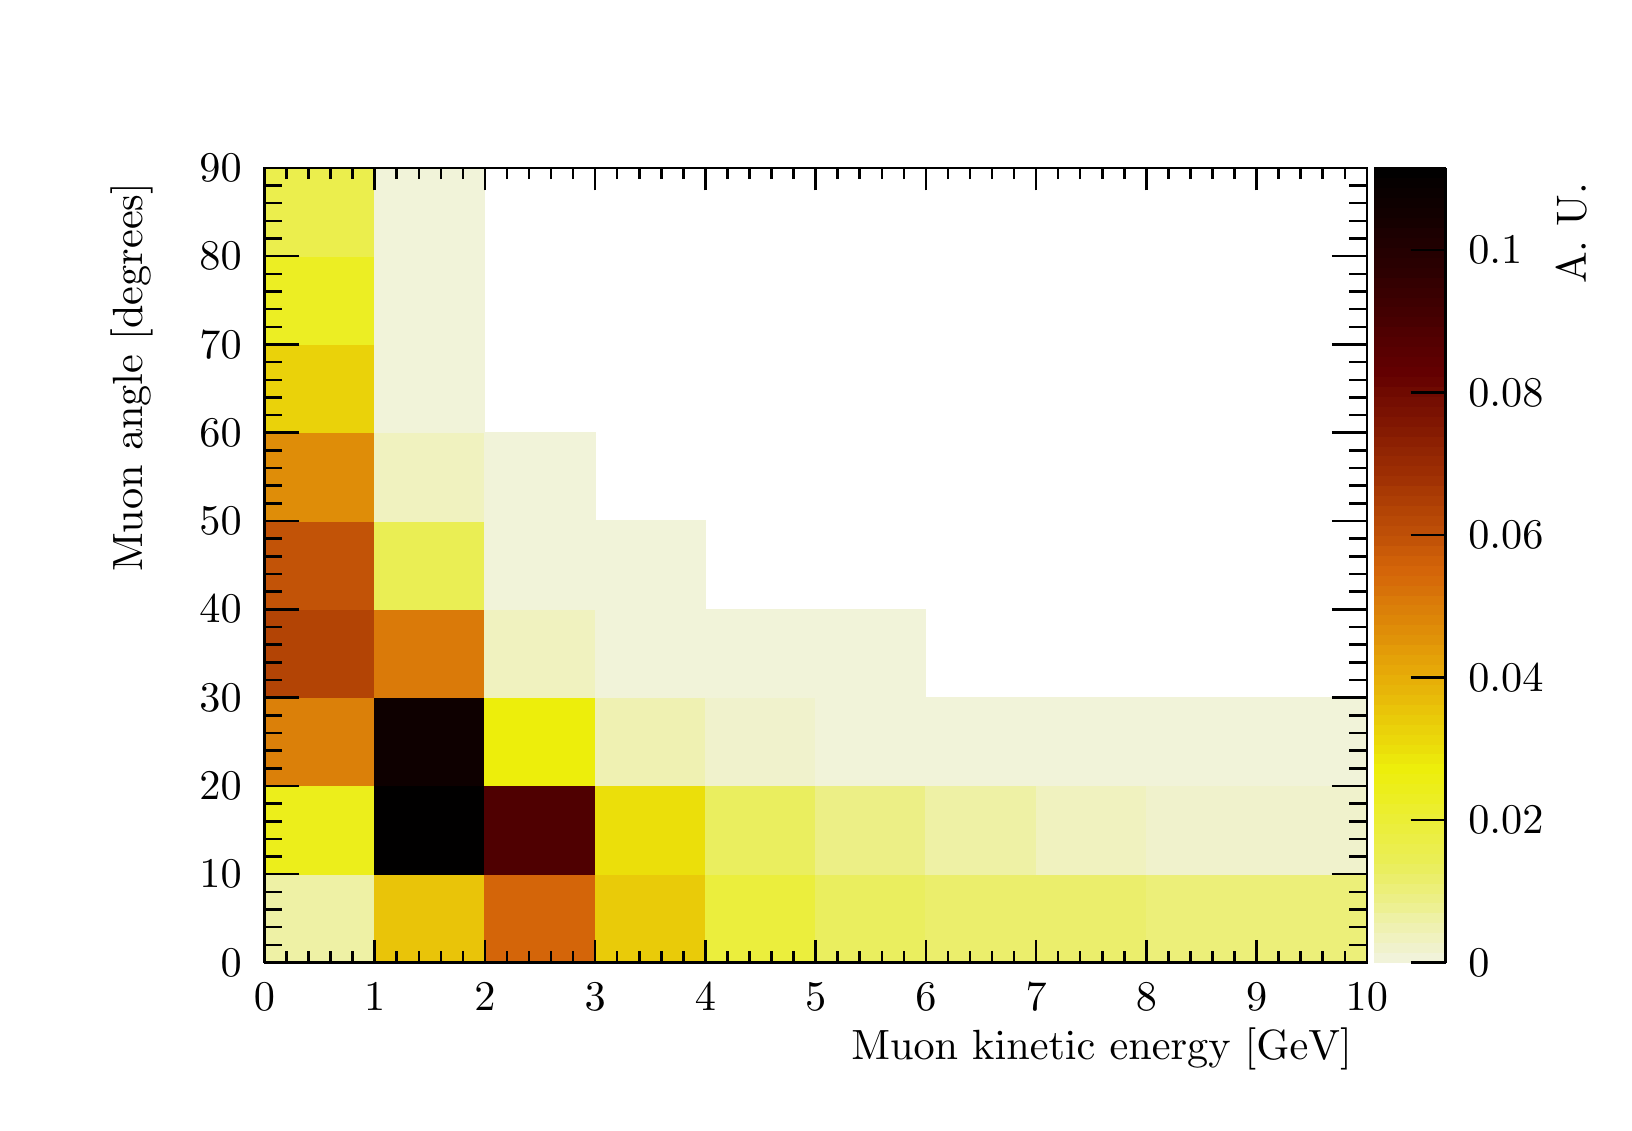
\begin{tikzpicture}
\pgfdeclareplotmark{cross} {
\pgfpathmoveto{\pgfpoint{-0.3\pgfplotmarksize}{\pgfplotmarksize}}
\pgfpathlineto{\pgfpoint{+0.3\pgfplotmarksize}{\pgfplotmarksize}}
\pgfpathlineto{\pgfpoint{+0.3\pgfplotmarksize}{0.3\pgfplotmarksize}}
\pgfpathlineto{\pgfpoint{+1\pgfplotmarksize}{0.3\pgfplotmarksize}}
\pgfpathlineto{\pgfpoint{+1\pgfplotmarksize}{-0.3\pgfplotmarksize}}
\pgfpathlineto{\pgfpoint{+0.3\pgfplotmarksize}{-0.3\pgfplotmarksize}}
\pgfpathlineto{\pgfpoint{+0.3\pgfplotmarksize}{-1.\pgfplotmarksize}}
\pgfpathlineto{\pgfpoint{-0.3\pgfplotmarksize}{-1.\pgfplotmarksize}}
\pgfpathlineto{\pgfpoint{-0.3\pgfplotmarksize}{-0.3\pgfplotmarksize}}
\pgfpathlineto{\pgfpoint{-1.\pgfplotmarksize}{-0.3\pgfplotmarksize}}
\pgfpathlineto{\pgfpoint{-1.\pgfplotmarksize}{0.3\pgfplotmarksize}}
\pgfpathlineto{\pgfpoint{-0.3\pgfplotmarksize}{0.3\pgfplotmarksize}}
\pgfpathclose
\pgfusepathqstroke
}
\pgfdeclareplotmark{cross*} {
\pgfpathmoveto{\pgfpoint{-0.3\pgfplotmarksize}{\pgfplotmarksize}}
\pgfpathlineto{\pgfpoint{+0.3\pgfplotmarksize}{\pgfplotmarksize}}
\pgfpathlineto{\pgfpoint{+0.3\pgfplotmarksize}{0.3\pgfplotmarksize}}
\pgfpathlineto{\pgfpoint{+1\pgfplotmarksize}{0.3\pgfplotmarksize}}
\pgfpathlineto{\pgfpoint{+1\pgfplotmarksize}{-0.3\pgfplotmarksize}}
\pgfpathlineto{\pgfpoint{+0.3\pgfplotmarksize}{-0.3\pgfplotmarksize}}
\pgfpathlineto{\pgfpoint{+0.3\pgfplotmarksize}{-1.\pgfplotmarksize}}
\pgfpathlineto{\pgfpoint{-0.3\pgfplotmarksize}{-1.\pgfplotmarksize}}
\pgfpathlineto{\pgfpoint{-0.3\pgfplotmarksize}{-0.3\pgfplotmarksize}}
\pgfpathlineto{\pgfpoint{-1.\pgfplotmarksize}{-0.3\pgfplotmarksize}}
\pgfpathlineto{\pgfpoint{-1.\pgfplotmarksize}{0.3\pgfplotmarksize}}
\pgfpathlineto{\pgfpoint{-0.3\pgfplotmarksize}{0.3\pgfplotmarksize}}
\pgfpathclose
\pgfusepathqfillstroke
}
\pgfdeclareplotmark{newstar} {
\pgfpathmoveto{\pgfqpoint{0pt}{\pgfplotmarksize}}
\pgfpathlineto{\pgfqpointpolar{44}{0.5\pgfplotmarksize}}
\pgfpathlineto{\pgfqpointpolar{18}{\pgfplotmarksize}}
\pgfpathlineto{\pgfqpointpolar{-20}{0.5\pgfplotmarksize}}
\pgfpathlineto{\pgfqpointpolar{-54}{\pgfplotmarksize}}
\pgfpathlineto{\pgfqpointpolar{-90}{0.5\pgfplotmarksize}}
\pgfpathlineto{\pgfqpointpolar{234}{\pgfplotmarksize}}
\pgfpathlineto{\pgfqpointpolar{198}{0.5\pgfplotmarksize}}
\pgfpathlineto{\pgfqpointpolar{162}{\pgfplotmarksize}}
\pgfpathlineto{\pgfqpointpolar{134}{0.5\pgfplotmarksize}}
\pgfpathclose
\pgfusepathqstroke
}
\pgfdeclareplotmark{newstar*} {
\pgfpathmoveto{\pgfqpoint{0pt}{\pgfplotmarksize}}
\pgfpathlineto{\pgfqpointpolar{44}{0.5\pgfplotmarksize}}
\pgfpathlineto{\pgfqpointpolar{18}{\pgfplotmarksize}}
\pgfpathlineto{\pgfqpointpolar{-20}{0.5\pgfplotmarksize}}
\pgfpathlineto{\pgfqpointpolar{-54}{\pgfplotmarksize}}
\pgfpathlineto{\pgfqpointpolar{-90}{0.5\pgfplotmarksize}}
\pgfpathlineto{\pgfqpointpolar{234}{\pgfplotmarksize}}
\pgfpathlineto{\pgfqpointpolar{198}{0.5\pgfplotmarksize}}
\pgfpathlineto{\pgfqpointpolar{162}{\pgfplotmarksize}}
\pgfpathlineto{\pgfqpointpolar{134}{0.5\pgfplotmarksize}}
\pgfpathclose
\pgfusepathqfillstroke
}
\definecolor{c}{rgb}{1,1,1};
\draw [color=c, fill=c] (0,0) rectangle (20,13.639);
\draw [color=c, fill=c] (3,1.77307) rectangle (17,11.8659);
\definecolor{c}{rgb}{0,0,0};
\draw [c,line width=0.9] (3,1.77307) -- (3,11.8659) -- (17,11.8659) -- (17,1.77307) -- (3,1.77307);
\definecolor{c}{rgb}{1,1,1};
\draw [color=c, fill=c] (3,1.77307) rectangle (17,11.8659);
\definecolor{c}{rgb}{0,0,0};
\draw [c,line width=0.9] (3,1.77307) -- (3,11.8659) -- (17,11.8659) -- (17,1.77307) -- (3,1.77307);
\definecolor{c}{rgb}{0.933839,0.943453,0.645794};
\draw [color=c, fill=c] (3,1.77307) rectangle (4.4,2.89449);
\definecolor{c}{rgb}{0.913113,0.770343,0.036152};
\draw [color=c, fill=c] (4.4,1.77307) rectangle (5.8,2.89449);
\definecolor{c}{rgb}{0.831373,0.396078,0.0352941};
\draw [color=c, fill=c] (5.8,1.77307) rectangle (7.2,2.89449);
\definecolor{c}{rgb}{0.915686,0.796078,0.0372549};
\draw [color=c, fill=c] (7.2,1.77307) rectangle (8.6,2.89449);
\definecolor{c}{rgb}{0.922426,0.933333,0.238725};
\draw [color=c, fill=c] (8.6,1.77307) rectangle (10,2.89449);
\definecolor{c}{rgb}{0.917647,0.933333,0.372549};
\draw [color=c, fill=c] (10,1.77307) rectangle (11.4,2.89449);
\definecolor{c}{rgb}{0.920683,0.935231,0.423782};
\draw [color=c, fill=c] (11.4,1.77307) rectangle (12.8,2.89449);
\draw [color=c, fill=c] (12.8,1.77307) rectangle (14.2,2.89449);
\definecolor{c}{rgb}{0.923719,0.937128,0.475016};
\draw [color=c, fill=c] (14.2,1.77307) rectangle (15.6,2.89449);
\draw [color=c, fill=c] (15.6,1.77307) rectangle (17,2.89449);
\definecolor{c}{rgb}{0.927206,0.933333,0.104902};
\draw [color=c, fill=c] (3,2.89449) rectangle (4.4,4.01592);
\definecolor{c}{rgb}{0.00551471,0,0.000122549};
\draw [color=c, fill=c] (4.4,2.89449) rectangle (5.8,4.01592);
\definecolor{c}{rgb}{0.308824,0,0.00392157};
\draw [color=c, fill=c] (5.8,2.89449) rectangle (7.2,4.01592);
\definecolor{c}{rgb}{0.923407,0.873284,0.0405637};
\draw [color=c, fill=c] (7.2,2.89449) rectangle (8.6,4.01592);
\definecolor{c}{rgb}{0.917647,0.933333,0.372549};
\draw [color=c, fill=c] (8.6,2.89449) rectangle (10,4.01592);
\definecolor{c}{rgb}{0.926755,0.939026,0.526249};
\draw [color=c, fill=c] (10,2.89449) rectangle (11.4,4.01592);
\definecolor{c}{rgb}{0.933839,0.943453,0.645794};
\draw [color=c, fill=c] (11.4,2.89449) rectangle (12.8,4.01592);
\definecolor{c}{rgb}{0.939911,0.947249,0.748261};
\draw [color=c, fill=c] (12.8,2.89449) rectangle (14.2,4.01592);
\definecolor{c}{rgb}{0.942948,0.949146,0.799494};
\draw [color=c, fill=c] (14.2,2.89449) rectangle (15.6,4.01592);
\draw [color=c, fill=c] (15.6,2.89449) rectangle (17,4.01592);
\definecolor{c}{rgb}{0.860049,0.502819,0.033701};
\draw [color=c, fill=c] (3,4.01592) rectangle (4.4,5.13734);
\definecolor{c}{rgb}{0.0551471,0,0.00122549};
\draw [color=c, fill=c] (4.4,4.01592) rectangle (5.8,5.13734);
\definecolor{c}{rgb}{0.929412,0.933333,0.0431373};
\draw [color=c, fill=c] (5.8,4.01592) rectangle (7.2,5.13734);
\definecolor{c}{rgb}{0.936875,0.945351,0.697027};
\draw [color=c, fill=c] (7.2,4.01592) rectangle (8.6,5.13734);
\definecolor{c}{rgb}{0.942948,0.949146,0.799494};
\draw [color=c, fill=c] (8.6,4.01592) rectangle (10,5.13734);
\definecolor{c}{rgb}{0.945984,0.951044,0.850727};
\draw [color=c, fill=c] (10,4.01592) rectangle (11.4,5.13734);
\draw [color=c, fill=c] (11.4,4.01592) rectangle (12.8,5.13734);
\draw [color=c, fill=c] (12.8,4.01592) rectangle (14.2,5.13734);
\draw [color=c, fill=c] (14.2,4.01592) rectangle (15.6,5.13734);
\draw [color=c, fill=c] (15.6,4.01592) rectangle (17,5.13734);
\definecolor{c}{rgb}{0.70098,0.265686,0.0213235};
\draw [color=c, fill=c] (3,5.13734) rectangle (4.4,6.25877);
\definecolor{c}{rgb}{0.853431,0.478186,0.0340686};
\draw [color=c, fill=c] (4.4,5.13734) rectangle (5.8,6.25877);
\definecolor{c}{rgb}{0.939911,0.947249,0.748261};
\draw [color=c, fill=c] (5.8,5.13734) rectangle (7.2,6.25877);
\definecolor{c}{rgb}{0.945984,0.951044,0.850727};
\draw [color=c, fill=c] (7.2,5.13734) rectangle (8.6,6.25877);
\draw [color=c, fill=c] (8.6,5.13734) rectangle (10,6.25877);
\draw [color=c, fill=c] (10,5.13734) rectangle (11.4,6.25877);
\definecolor{c}{rgb}{0.762745,0.327451,0.0279412};
\draw [color=c, fill=c] (3,6.25877) rectangle (4.4,7.3802);
\definecolor{c}{rgb}{0.919118,0.933333,0.331373};
\draw [color=c, fill=c] (4.4,6.25877) rectangle (5.8,7.3802);
\definecolor{c}{rgb}{0.945984,0.951044,0.850727};
\draw [color=c, fill=c] (5.8,6.25877) rectangle (7.2,7.3802);
\draw [color=c, fill=c] (7.2,6.25877) rectangle (8.6,7.3802);
\definecolor{c}{rgb}{0.873284,0.552083,0.0329657};
\draw [color=c, fill=c] (3,7.3802) rectangle (4.4,8.50162);
\definecolor{c}{rgb}{0.939911,0.947249,0.748261};
\draw [color=c, fill=c] (4.4,7.3802) rectangle (5.8,8.50162);
\definecolor{c}{rgb}{0.945984,0.951044,0.850727};
\draw [color=c, fill=c] (5.8,7.3802) rectangle (7.2,8.50162);
\definecolor{c}{rgb}{0.91826,0.821814,0.0383578};
\draw [color=c, fill=c] (3,8.50162) rectangle (4.4,9.62305);
\definecolor{c}{rgb}{0.945984,0.951044,0.850727};
\draw [color=c, fill=c] (4.4,8.50162) rectangle (5.8,9.62305);
\definecolor{c}{rgb}{0.926103,0.933333,0.135784};
\draw [color=c, fill=c] (3,9.62305) rectangle (4.4,10.7445);
\definecolor{c}{rgb}{0.945984,0.951044,0.850727};
\draw [color=c, fill=c] (4.4,9.62305) rectangle (5.8,10.7445);
\definecolor{c}{rgb}{0.920221,0.933333,0.30049};
\draw [color=c, fill=c] (3,10.7445) rectangle (4.4,11.8659);
\definecolor{c}{rgb}{0.945984,0.951044,0.850727};
\draw [color=c, fill=c] (4.4,10.7445) rectangle (5.8,11.8659);
\definecolor{c}{rgb}{0,0,0};
\draw [c,line width=0.9] (3,1.77307) -- (17,1.77307);
\draw [c,line width=0.9] (3,2.05948) -- (3,1.77307);
\draw [c,line width=0.9] (3.28,1.91628) -- (3.28,1.77307);
\draw [c,line width=0.9] (3.56,1.91628) -- (3.56,1.77307);
\draw [c,line width=0.9] (3.84,1.91628) -- (3.84,1.77307);
\draw [c,line width=0.9] (4.12,1.91628) -- (4.12,1.77307);
\draw [c,line width=0.9] (4.4,2.05948) -- (4.4,1.77307);
\draw [c,line width=0.9] (4.68,1.91628) -- (4.68,1.77307);
\draw [c,line width=0.9] (4.96,1.91628) -- (4.96,1.77307);
\draw [c,line width=0.9] (5.24,1.91628) -- (5.24,1.77307);
\draw [c,line width=0.9] (5.52,1.91628) -- (5.52,1.77307);
\draw [c,line width=0.9] (5.8,2.05948) -- (5.8,1.77307);
\draw [c,line width=0.9] (6.08,1.91628) -- (6.08,1.77307);
\draw [c,line width=0.9] (6.36,1.91628) -- (6.36,1.77307);
\draw [c,line width=0.9] (6.64,1.91628) -- (6.64,1.77307);
\draw [c,line width=0.9] (6.92,1.91628) -- (6.92,1.77307);
\draw [c,line width=0.9] (7.2,2.05948) -- (7.2,1.77307);
\draw [c,line width=0.9] (7.48,1.91628) -- (7.48,1.77307);
\draw [c,line width=0.9] (7.76,1.91628) -- (7.76,1.77307);
\draw [c,line width=0.9] (8.04,1.91628) -- (8.04,1.77307);
\draw [c,line width=0.9] (8.32,1.91628) -- (8.32,1.77307);
\draw [c,line width=0.9] (8.6,2.05948) -- (8.6,1.77307);
\draw [c,line width=0.9] (8.88,1.91628) -- (8.88,1.77307);
\draw [c,line width=0.9] (9.16,1.91628) -- (9.16,1.77307);
\draw [c,line width=0.9] (9.44,1.91628) -- (9.44,1.77307);
\draw [c,line width=0.9] (9.72,1.91628) -- (9.72,1.77307);
\draw [c,line width=0.9] (10,2.05948) -- (10,1.77307);
\draw [c,line width=0.9] (10.28,1.91628) -- (10.28,1.77307);
\draw [c,line width=0.9] (10.56,1.91628) -- (10.56,1.77307);
\draw [c,line width=0.9] (10.84,1.91628) -- (10.84,1.77307);
\draw [c,line width=0.9] (11.12,1.91628) -- (11.12,1.77307);
\draw [c,line width=0.9] (11.4,2.05948) -- (11.4,1.77307);
\draw [c,line width=0.9] (11.68,1.91628) -- (11.68,1.77307);
\draw [c,line width=0.9] (11.96,1.91628) -- (11.96,1.77307);
\draw [c,line width=0.9] (12.24,1.91628) -- (12.24,1.77307);
\draw [c,line width=0.9] (12.52,1.91628) -- (12.52,1.77307);
\draw [c,line width=0.9] (12.8,2.05948) -- (12.8,1.77307);
\draw [c,line width=0.9] (13.08,1.91628) -- (13.08,1.77307);
\draw [c,line width=0.9] (13.36,1.91628) -- (13.36,1.77307);
\draw [c,line width=0.9] (13.64,1.91628) -- (13.64,1.77307);
\draw [c,line width=0.9] (13.92,1.91628) -- (13.92,1.77307);
\draw [c,line width=0.9] (14.2,2.05948) -- (14.2,1.77307);
\draw [c,line width=0.9] (14.48,1.91628) -- (14.48,1.77307);
\draw [c,line width=0.9] (14.76,1.91628) -- (14.76,1.77307);
\draw [c,line width=0.9] (15.04,1.91628) -- (15.04,1.77307);
\draw [c,line width=0.9] (15.32,1.91628) -- (15.32,1.77307);
\draw [c,line width=0.9] (15.6,2.05948) -- (15.6,1.77307);
\draw [c,line width=0.9] (15.88,1.91628) -- (15.88,1.77307);
\draw [c,line width=0.9] (16.16,1.91628) -- (16.16,1.77307);
\draw [c,line width=0.9] (16.44,1.91628) -- (16.44,1.77307);
\draw [c,line width=0.9] (16.72,1.91628) -- (16.72,1.77307);
\draw [c,line width=0.9] (17,2.05948) -- (17,1.77307);
\draw [anchor=base] (3,1.15931) node[scale=1.52731, color=c, rotate=0]{0};
\draw [anchor=base] (4.4,1.15931) node[scale=1.52731, color=c, rotate=0]{1};
\draw [anchor=base] (5.8,1.15931) node[scale=1.52731, color=c, rotate=0]{2};
\draw [anchor=base] (7.2,1.15931) node[scale=1.52731, color=c, rotate=0]{3};
\draw [anchor=base] (8.6,1.15931) node[scale=1.52731, color=c, rotate=0]{4};
\draw [anchor=base] (10,1.15931) node[scale=1.52731, color=c, rotate=0]{5};
\draw [anchor=base] (11.4,1.15931) node[scale=1.52731, color=c, rotate=0]{6};
\draw [anchor=base] (12.8,1.15931) node[scale=1.52731, color=c, rotate=0]{7};
\draw [anchor=base] (14.2,1.15931) node[scale=1.52731, color=c, rotate=0]{8};
\draw [anchor=base] (15.6,1.15931) node[scale=1.52731, color=c, rotate=0]{9};
\draw [anchor=base] (17,1.15931) node[scale=1.52731, color=c, rotate=0]{10};
\draw [anchor= east] (17,0.681948) node[scale=1.52731, color=c, rotate=0]{ Muon kinetic energy [GeV]};
\draw [c,line width=0.9] (3,11.8659) -- (17,11.8659);
\draw [c,line width=0.9] (3,11.5795) -- (3,11.8659);
\draw [c,line width=0.9] (3.28,11.7227) -- (3.28,11.8659);
\draw [c,line width=0.9] (3.56,11.7227) -- (3.56,11.8659);
\draw [c,line width=0.9] (3.84,11.7227) -- (3.84,11.8659);
\draw [c,line width=0.9] (4.12,11.7227) -- (4.12,11.8659);
\draw [c,line width=0.9] (4.4,11.5795) -- (4.4,11.8659);
\draw [c,line width=0.9] (4.68,11.7227) -- (4.68,11.8659);
\draw [c,line width=0.9] (4.96,11.7227) -- (4.96,11.8659);
\draw [c,line width=0.9] (5.24,11.7227) -- (5.24,11.8659);
\draw [c,line width=0.9] (5.52,11.7227) -- (5.52,11.8659);
\draw [c,line width=0.9] (5.8,11.5795) -- (5.8,11.8659);
\draw [c,line width=0.9] (6.08,11.7227) -- (6.08,11.8659);
\draw [c,line width=0.9] (6.36,11.7227) -- (6.36,11.8659);
\draw [c,line width=0.9] (6.64,11.7227) -- (6.64,11.8659);
\draw [c,line width=0.9] (6.92,11.7227) -- (6.92,11.8659);
\draw [c,line width=0.9] (7.2,11.5795) -- (7.2,11.8659);
\draw [c,line width=0.9] (7.48,11.7227) -- (7.48,11.8659);
\draw [c,line width=0.9] (7.76,11.7227) -- (7.76,11.8659);
\draw [c,line width=0.9] (8.04,11.7227) -- (8.04,11.8659);
\draw [c,line width=0.9] (8.32,11.7227) -- (8.32,11.8659);
\draw [c,line width=0.9] (8.6,11.5795) -- (8.6,11.8659);
\draw [c,line width=0.9] (8.88,11.7227) -- (8.88,11.8659);
\draw [c,line width=0.9] (9.16,11.7227) -- (9.16,11.8659);
\draw [c,line width=0.9] (9.44,11.7227) -- (9.44,11.8659);
\draw [c,line width=0.9] (9.72,11.7227) -- (9.72,11.8659);
\draw [c,line width=0.9] (10,11.5795) -- (10,11.8659);
\draw [c,line width=0.9] (10.28,11.7227) -- (10.28,11.8659);
\draw [c,line width=0.9] (10.56,11.7227) -- (10.56,11.8659);
\draw [c,line width=0.9] (10.84,11.7227) -- (10.84,11.8659);
\draw [c,line width=0.9] (11.12,11.7227) -- (11.12,11.8659);
\draw [c,line width=0.9] (11.4,11.5795) -- (11.4,11.8659);
\draw [c,line width=0.9] (11.68,11.7227) -- (11.68,11.8659);
\draw [c,line width=0.9] (11.96,11.7227) -- (11.96,11.8659);
\draw [c,line width=0.9] (12.24,11.7227) -- (12.24,11.8659);
\draw [c,line width=0.9] (12.52,11.7227) -- (12.52,11.8659);
\draw [c,line width=0.9] (12.8,11.5795) -- (12.8,11.8659);
\draw [c,line width=0.9] (13.08,11.7227) -- (13.08,11.8659);
\draw [c,line width=0.9] (13.36,11.7227) -- (13.36,11.8659);
\draw [c,line width=0.9] (13.64,11.7227) -- (13.64,11.8659);
\draw [c,line width=0.9] (13.92,11.7227) -- (13.92,11.8659);
\draw [c,line width=0.9] (14.2,11.5795) -- (14.2,11.8659);
\draw [c,line width=0.9] (14.48,11.7227) -- (14.48,11.8659);
\draw [c,line width=0.9] (14.76,11.7227) -- (14.76,11.8659);
\draw [c,line width=0.9] (15.04,11.7227) -- (15.04,11.8659);
\draw [c,line width=0.9] (15.32,11.7227) -- (15.32,11.8659);
\draw [c,line width=0.9] (15.6,11.5795) -- (15.6,11.8659);
\draw [c,line width=0.9] (15.88,11.7227) -- (15.88,11.8659);
\draw [c,line width=0.9] (16.16,11.7227) -- (16.16,11.8659);
\draw [c,line width=0.9] (16.44,11.7227) -- (16.44,11.8659);
\draw [c,line width=0.9] (16.72,11.7227) -- (16.72,11.8659);
\draw [c,line width=0.9] (17,11.5795) -- (17,11.8659);
\draw [c,line width=0.9] (3,1.77307) -- (3,11.8659);
\draw [c,line width=0.9] (3.444,1.77307) -- (3,1.77307);
\draw [c,line width=0.9] (3.222,1.99735) -- (3,1.99735);
\draw [c,line width=0.9] (3.222,2.22164) -- (3,2.22164);
\draw [c,line width=0.9] (3.222,2.44592) -- (3,2.44592);
\draw [c,line width=0.9] (3.222,2.67021) -- (3,2.67021);
\draw [c,line width=0.9] (3.444,2.89449) -- (3,2.89449);
\draw [c,line width=0.9] (3.222,3.11878) -- (3,3.11878);
\draw [c,line width=0.9] (3.222,3.34306) -- (3,3.34306);
\draw [c,line width=0.9] (3.222,3.56735) -- (3,3.56735);
\draw [c,line width=0.9] (3.222,3.79163) -- (3,3.79163);
\draw [c,line width=0.9] (3.444,4.01592) -- (3,4.01592);
\draw [c,line width=0.9] (3.222,4.2402) -- (3,4.2402);
\draw [c,line width=0.9] (3.222,4.46449) -- (3,4.46449);
\draw [c,line width=0.9] (3.222,4.68877) -- (3,4.68877);
\draw [c,line width=0.9] (3.222,4.91306) -- (3,4.91306);
\draw [c,line width=0.9] (3.444,5.13734) -- (3,5.13734);
\draw [c,line width=0.9] (3.222,5.36163) -- (3,5.36163);
\draw [c,line width=0.9] (3.222,5.58592) -- (3,5.58592);
\draw [c,line width=0.9] (3.222,5.8102) -- (3,5.8102);
\draw [c,line width=0.9] (3.222,6.03449) -- (3,6.03449);
\draw [c,line width=0.9] (3.444,6.25877) -- (3,6.25877);
\draw [c,line width=0.9] (3.222,6.48306) -- (3,6.48306);
\draw [c,line width=0.9] (3.222,6.70734) -- (3,6.70734);
\draw [c,line width=0.9] (3.222,6.93163) -- (3,6.93163);
\draw [c,line width=0.9] (3.222,7.15591) -- (3,7.15591);
\draw [c,line width=0.9] (3.444,7.3802) -- (3,7.3802);
\draw [c,line width=0.9] (3.222,7.60448) -- (3,7.60448);
\draw [c,line width=0.9] (3.222,7.82877) -- (3,7.82877);
\draw [c,line width=0.9] (3.222,8.05305) -- (3,8.05305);
\draw [c,line width=0.9] (3.222,8.27734) -- (3,8.27734);
\draw [c,line width=0.9] (3.444,8.50162) -- (3,8.50162);
\draw [c,line width=0.9] (3.222,8.72591) -- (3,8.72591);
\draw [c,line width=0.9] (3.222,8.95019) -- (3,8.95019);
\draw [c,line width=0.9] (3.222,9.17448) -- (3,9.17448);
\draw [c,line width=0.9] (3.222,9.39876) -- (3,9.39876);
\draw [c,line width=0.9] (3.444,9.62305) -- (3,9.62305);
\draw [c,line width=0.9] (3.222,9.84733) -- (3,9.84733);
\draw [c,line width=0.9] (3.222,10.0716) -- (3,10.0716);
\draw [c,line width=0.9] (3.222,10.2959) -- (3,10.2959);
\draw [c,line width=0.9] (3.222,10.5202) -- (3,10.5202);
\draw [c,line width=0.9] (3.444,10.7445) -- (3,10.7445);
\draw [c,line width=0.9] (3.222,10.9688) -- (3,10.9688);
\draw [c,line width=0.9] (3.222,11.193) -- (3,11.193);
\draw [c,line width=0.9] (3.222,11.4173) -- (3,11.4173);
\draw [c,line width=0.9] (3.222,11.6416) -- (3,11.6416);
\draw [c,line width=0.9] (3.444,11.8659) -- (3,11.8659);
\draw [anchor= east] (2.9,1.77307) node[scale=1.52731, color=c, rotate=0]{0};
\draw [anchor= east] (2.9,2.89449) node[scale=1.52731, color=c, rotate=0]{10};
\draw [anchor= east] (2.9,4.01592) node[scale=1.52731, color=c, rotate=0]{20};
\draw [anchor= east] (2.9,5.13734) node[scale=1.52731, color=c, rotate=0]{30};
\draw [anchor= east] (2.9,6.25877) node[scale=1.52731, color=c, rotate=0]{40};
\draw [anchor= east] (2.9,7.3802) node[scale=1.52731, color=c, rotate=0]{50};
\draw [anchor= east] (2.9,8.50162) node[scale=1.52731, color=c, rotate=0]{60};
\draw [anchor= east] (2.9,9.62305) node[scale=1.52731, color=c, rotate=0]{70};
\draw [anchor= east] (2.9,10.7445) node[scale=1.52731, color=c, rotate=0]{80};
\draw [anchor= east] (2.9,11.8659) node[scale=1.52731, color=c, rotate=0]{90};
\draw [anchor= east] (1.31232,11.8659) node[scale=1.52731, color=c, rotate=90]{ Muon angle [degrees]};
\draw [c,line width=0.9] (17,1.77307) -- (17,11.8659);
\draw [c,line width=0.9] (16.556,1.77307) -- (17,1.77307);
\draw [c,line width=0.9] (16.778,1.99735) -- (17,1.99735);
\draw [c,line width=0.9] (16.778,2.22164) -- (17,2.22164);
\draw [c,line width=0.9] (16.778,2.44592) -- (17,2.44592);
\draw [c,line width=0.9] (16.778,2.67021) -- (17,2.67021);
\draw [c,line width=0.9] (16.556,2.89449) -- (17,2.89449);
\draw [c,line width=0.9] (16.778,3.11878) -- (17,3.11878);
\draw [c,line width=0.9] (16.778,3.34306) -- (17,3.34306);
\draw [c,line width=0.9] (16.778,3.56735) -- (17,3.56735);
\draw [c,line width=0.9] (16.778,3.79163) -- (17,3.79163);
\draw [c,line width=0.9] (16.556,4.01592) -- (17,4.01592);
\draw [c,line width=0.9] (16.778,4.2402) -- (17,4.2402);
\draw [c,line width=0.9] (16.778,4.46449) -- (17,4.46449);
\draw [c,line width=0.9] (16.778,4.68877) -- (17,4.68877);
\draw [c,line width=0.9] (16.778,4.91306) -- (17,4.91306);
\draw [c,line width=0.9] (16.556,5.13734) -- (17,5.13734);
\draw [c,line width=0.9] (16.778,5.36163) -- (17,5.36163);
\draw [c,line width=0.9] (16.778,5.58592) -- (17,5.58592);
\draw [c,line width=0.9] (16.778,5.8102) -- (17,5.8102);
\draw [c,line width=0.9] (16.778,6.03449) -- (17,6.03449);
\draw [c,line width=0.9] (16.556,6.25877) -- (17,6.25877);
\draw [c,line width=0.9] (16.778,6.48306) -- (17,6.48306);
\draw [c,line width=0.9] (16.778,6.70734) -- (17,6.70734);
\draw [c,line width=0.9] (16.778,6.93163) -- (17,6.93163);
\draw [c,line width=0.9] (16.778,7.15591) -- (17,7.15591);
\draw [c,line width=0.9] (16.556,7.3802) -- (17,7.3802);
\draw [c,line width=0.9] (16.778,7.60448) -- (17,7.60448);
\draw [c,line width=0.9] (16.778,7.82877) -- (17,7.82877);
\draw [c,line width=0.9] (16.778,8.05305) -- (17,8.05305);
\draw [c,line width=0.9] (16.778,8.27734) -- (17,8.27734);
\draw [c,line width=0.9] (16.556,8.50162) -- (17,8.50162);
\draw [c,line width=0.9] (16.778,8.72591) -- (17,8.72591);
\draw [c,line width=0.9] (16.778,8.95019) -- (17,8.95019);
\draw [c,line width=0.9] (16.778,9.17448) -- (17,9.17448);
\draw [c,line width=0.9] (16.778,9.39876) -- (17,9.39876);
\draw [c,line width=0.9] (16.556,9.62305) -- (17,9.62305);
\draw [c,line width=0.9] (16.778,9.84733) -- (17,9.84733);
\draw [c,line width=0.9] (16.778,10.0716) -- (17,10.0716);
\draw [c,line width=0.9] (16.778,10.2959) -- (17,10.2959);
\draw [c,line width=0.9] (16.778,10.5202) -- (17,10.5202);
\draw [c,line width=0.9] (16.556,10.7445) -- (17,10.7445);
\draw [c,line width=0.9] (16.778,10.9688) -- (17,10.9688);
\draw [c,line width=0.9] (16.778,11.193) -- (17,11.193);
\draw [c,line width=0.9] (16.778,11.4173) -- (17,11.4173);
\draw [c,line width=0.9] (16.778,11.6416) -- (17,11.6416);
\draw [c,line width=0.9] (16.556,11.8659) -- (17,11.8659);
\definecolor{c}{rgb}{0.945984,0.951044,0.850727};
\draw [color=c, fill=c] (17.1,1.77307) rectangle (18,1.89923);
\definecolor{c}{rgb}{0.942948,0.949146,0.799494};
\draw [color=c, fill=c] (17.1,1.89923) rectangle (18,2.02539);
\definecolor{c}{rgb}{0.939911,0.947249,0.748261};
\draw [color=c, fill=c] (17.1,2.02539) rectangle (18,2.15155);
\definecolor{c}{rgb}{0.936875,0.945351,0.697027};
\draw [color=c, fill=c] (17.1,2.15155) rectangle (18,2.27771);
\definecolor{c}{rgb}{0.933839,0.943453,0.645794};
\draw [color=c, fill=c] (17.1,2.27771) rectangle (18,2.40387);
\definecolor{c}{rgb}{0.929791,0.940923,0.577483};
\draw [color=c, fill=c] (17.1,2.40387) rectangle (18,2.53003);
\definecolor{c}{rgb}{0.926755,0.939026,0.526249};
\draw [color=c, fill=c] (17.1,2.53003) rectangle (18,2.65619);
\definecolor{c}{rgb}{0.923719,0.937128,0.475016};
\draw [color=c, fill=c] (17.1,2.65619) rectangle (18,2.78235);
\definecolor{c}{rgb}{0.920683,0.935231,0.423782};
\draw [color=c, fill=c] (17.1,2.78235) rectangle (18,2.90851);
\definecolor{c}{rgb}{0.917647,0.933333,0.372549};
\draw [color=c, fill=c] (17.1,2.90851) rectangle (18,3.03467);
\definecolor{c}{rgb}{0.919118,0.933333,0.331373};
\draw [color=c, fill=c] (17.1,3.03467) rectangle (18,3.16083);
\definecolor{c}{rgb}{0.920221,0.933333,0.30049};
\draw [color=c, fill=c] (17.1,3.16083) rectangle (18,3.28699);
\definecolor{c}{rgb}{0.921324,0.933333,0.269608};
\draw [color=c, fill=c] (17.1,3.28699) rectangle (18,3.41315);
\definecolor{c}{rgb}{0.922426,0.933333,0.238725};
\draw [color=c, fill=c] (17.1,3.41315) rectangle (18,3.53931);
\definecolor{c}{rgb}{0.923529,0.933333,0.207843};
\draw [color=c, fill=c] (17.1,3.53931) rectangle (18,3.66547);
\definecolor{c}{rgb}{0.924632,0.933333,0.176961};
\draw [color=c, fill=c] (17.1,3.66547) rectangle (18,3.79163);
\definecolor{c}{rgb}{0.926103,0.933333,0.135784};
\draw [color=c, fill=c] (17.1,3.79163) rectangle (18,3.91779);
\definecolor{c}{rgb}{0.927206,0.933333,0.104902};
\draw [color=c, fill=c] (17.1,3.91779) rectangle (18,4.04395);
\definecolor{c}{rgb}{0.928309,0.933333,0.0740196};
\draw [color=c, fill=c] (17.1,4.04395) rectangle (18,4.17011);
\definecolor{c}{rgb}{0.929412,0.933333,0.0431373};
\draw [color=c, fill=c] (17.1,4.17011) rectangle (18,4.29628);
\definecolor{c}{rgb}{0.926838,0.907598,0.0420343};
\draw [color=c, fill=c] (17.1,4.29628) rectangle (18,4.42244);
\definecolor{c}{rgb}{0.923407,0.873284,0.0405637};
\draw [color=c, fill=c] (17.1,4.42244) rectangle (18,4.5486);
\definecolor{c}{rgb}{0.920833,0.847549,0.0394608};
\draw [color=c, fill=c] (17.1,4.5486) rectangle (18,4.67476);
\definecolor{c}{rgb}{0.91826,0.821814,0.0383578};
\draw [color=c, fill=c] (17.1,4.67476) rectangle (18,4.80092);
\definecolor{c}{rgb}{0.915686,0.796078,0.0372549};
\draw [color=c, fill=c] (17.1,4.80092) rectangle (18,4.92708);
\definecolor{c}{rgb}{0.913113,0.770343,0.036152};
\draw [color=c, fill=c] (17.1,4.92708) rectangle (18,5.05324);
\definecolor{c}{rgb}{0.909681,0.736029,0.0346814};
\draw [color=c, fill=c] (17.1,5.05324) rectangle (18,5.1794);
\definecolor{c}{rgb}{0.907108,0.710294,0.0335784};
\draw [color=c, fill=c] (17.1,5.1794) rectangle (18,5.30556);
\definecolor{c}{rgb}{0.904534,0.684559,0.0324755};
\draw [color=c, fill=c] (17.1,5.30556) rectangle (18,5.43172);
\definecolor{c}{rgb}{0.901961,0.658824,0.0313726};
\draw [color=c, fill=c] (17.1,5.43172) rectangle (18,5.55788);
\definecolor{c}{rgb}{0.895343,0.634191,0.0317402};
\draw [color=c, fill=c] (17.1,5.55788) rectangle (18,5.68404);
\definecolor{c}{rgb}{0.888726,0.609559,0.0321078};
\draw [color=c, fill=c] (17.1,5.68404) rectangle (18,5.8102);
\definecolor{c}{rgb}{0.879902,0.576716,0.032598};
\draw [color=c, fill=c] (17.1,5.8102) rectangle (18,5.93636);
\definecolor{c}{rgb}{0.873284,0.552083,0.0329657};
\draw [color=c, fill=c] (17.1,5.93636) rectangle (18,6.06252);
\definecolor{c}{rgb}{0.866667,0.527451,0.0333333};
\draw [color=c, fill=c] (17.1,6.06252) rectangle (18,6.18868);
\definecolor{c}{rgb}{0.860049,0.502819,0.033701};
\draw [color=c, fill=c] (17.1,6.18868) rectangle (18,6.31484);
\definecolor{c}{rgb}{0.853431,0.478186,0.0340686};
\draw [color=c, fill=c] (17.1,6.31484) rectangle (18,6.441);
\definecolor{c}{rgb}{0.844608,0.445343,0.0345588};
\draw [color=c, fill=c] (17.1,6.441) rectangle (18,6.56716);
\definecolor{c}{rgb}{0.83799,0.420711,0.0349265};
\draw [color=c, fill=c] (17.1,6.56716) rectangle (18,6.69332);
\definecolor{c}{rgb}{0.831373,0.396078,0.0352941};
\draw [color=c, fill=c] (17.1,6.69332) rectangle (18,6.81948);
\definecolor{c}{rgb}{0.810784,0.37549,0.0330882};
\draw [color=c, fill=c] (17.1,6.81948) rectangle (18,6.94564);
\definecolor{c}{rgb}{0.790196,0.354902,0.0308824};
\draw [color=c, fill=c] (17.1,6.94564) rectangle (18,7.07181);
\definecolor{c}{rgb}{0.762745,0.327451,0.0279412};
\draw [color=c, fill=c] (17.1,7.07181) rectangle (18,7.19797);
\definecolor{c}{rgb}{0.742157,0.306863,0.0257353};
\draw [color=c, fill=c] (17.1,7.19797) rectangle (18,7.32413);
\definecolor{c}{rgb}{0.721569,0.286275,0.0235294};
\draw [color=c, fill=c] (17.1,7.32413) rectangle (18,7.45029);
\definecolor{c}{rgb}{0.70098,0.265686,0.0213235};
\draw [color=c, fill=c] (17.1,7.45029) rectangle (18,7.57645);
\definecolor{c}{rgb}{0.680392,0.245098,0.0191176};
\draw [color=c, fill=c] (17.1,7.57645) rectangle (18,7.70261);
\definecolor{c}{rgb}{0.659804,0.22451,0.0169118};
\draw [color=c, fill=c] (17.1,7.70261) rectangle (18,7.82877);
\definecolor{c}{rgb}{0.632353,0.197059,0.0139706};
\draw [color=c, fill=c] (17.1,7.82877) rectangle (18,7.95493);
\definecolor{c}{rgb}{0.611765,0.176471,0.0117647};
\draw [color=c, fill=c] (17.1,7.95493) rectangle (18,8.08109);
\definecolor{c}{rgb}{0.590809,0.159926,0.0110294};
\draw [color=c, fill=c] (17.1,8.08109) rectangle (18,8.20725);
\definecolor{c}{rgb}{0.569853,0.143382,0.0102941};
\draw [color=c, fill=c] (17.1,8.20725) rectangle (18,8.33341);
\definecolor{c}{rgb}{0.548897,0.126838,0.00955882};
\draw [color=c, fill=c] (17.1,8.33341) rectangle (18,8.45957);
\definecolor{c}{rgb}{0.520956,0.104779,0.00857843};
\draw [color=c, fill=c] (17.1,8.45957) rectangle (18,8.58573);
\definecolor{c}{rgb}{0.5,0.0882353,0.00784314};
\draw [color=c, fill=c] (17.1,8.58573) rectangle (18,8.71189);
\definecolor{c}{rgb}{0.479044,0.0716912,0.00710784};
\draw [color=c, fill=c] (17.1,8.71189) rectangle (18,8.83805);
\definecolor{c}{rgb}{0.458088,0.0551471,0.00637255};
\draw [color=c, fill=c] (17.1,8.83805) rectangle (18,8.96421);
\definecolor{c}{rgb}{0.437132,0.0386029,0.00563726};
\draw [color=c, fill=c] (17.1,8.96421) rectangle (18,9.09037);
\definecolor{c}{rgb}{0.409191,0.0165441,0.00465686};
\draw [color=c, fill=c] (17.1,9.09037) rectangle (18,9.21653);
\definecolor{c}{rgb}{0.388235,0,0.00392157};
\draw [color=c, fill=c] (17.1,9.21653) rectangle (18,9.34269);
\definecolor{c}{rgb}{0.368382,0,0.00392157};
\draw [color=c, fill=c] (17.1,9.34269) rectangle (18,9.46885);
\definecolor{c}{rgb}{0.348529,0,0.00392157};
\draw [color=c, fill=c] (17.1,9.46885) rectangle (18,9.59501);
\definecolor{c}{rgb}{0.328676,0,0.00392157};
\draw [color=c, fill=c] (17.1,9.59501) rectangle (18,9.72118);
\definecolor{c}{rgb}{0.308824,0,0.00392157};
\draw [color=c, fill=c] (17.1,9.72118) rectangle (18,9.84733);
\definecolor{c}{rgb}{0.282353,0,0.00392157};
\draw [color=c, fill=c] (17.1,9.84733) rectangle (18,9.9735);
\definecolor{c}{rgb}{0.2625,0,0.00392157};
\draw [color=c, fill=c] (17.1,9.9735) rectangle (18,10.0997);
\definecolor{c}{rgb}{0.242647,0,0.00392157};
\draw [color=c, fill=c] (17.1,10.0997) rectangle (18,10.2258);
\definecolor{c}{rgb}{0.222794,0,0.00392157};
\draw [color=c, fill=c] (17.1,10.2258) rectangle (18,10.352);
\definecolor{c}{rgb}{0.202941,0,0.00392157};
\draw [color=c, fill=c] (17.1,10.352) rectangle (18,10.4781);
\definecolor{c}{rgb}{0.176471,0,0.00392157};
\draw [color=c, fill=c] (17.1,10.4781) rectangle (18,10.6043);
\definecolor{c}{rgb}{0.159926,0,0.00355392};
\draw [color=c, fill=c] (17.1,10.6043) rectangle (18,10.7305);
\definecolor{c}{rgb}{0.143382,0,0.00318627};
\draw [color=c, fill=c] (17.1,10.7305) rectangle (18,10.8566);
\definecolor{c}{rgb}{0.126838,0,0.00281863};
\draw [color=c, fill=c] (17.1,10.8566) rectangle (18,10.9828);
\definecolor{c}{rgb}{0.110294,0,0.00245098};
\draw [color=c, fill=c] (17.1,10.9828) rectangle (18,11.1089);
\definecolor{c}{rgb}{0.0882353,0,0.00196078};
\draw [color=c, fill=c] (17.1,11.1089) rectangle (18,11.2351);
\definecolor{c}{rgb}{0.0716912,0,0.00159314};
\draw [color=c, fill=c] (17.1,11.2351) rectangle (18,11.3613);
\definecolor{c}{rgb}{0.0551471,0,0.00122549};
\draw [color=c, fill=c] (17.1,11.3613) rectangle (18,11.4874);
\definecolor{c}{rgb}{0.0386029,0,0.000857843};
\draw [color=c, fill=c] (17.1,11.4874) rectangle (18,11.6136);
\definecolor{c}{rgb}{0.0220588,0,0.000490196};
\draw [color=c, fill=c] (17.1,11.6136) rectangle (18,11.7397);
\definecolor{c}{rgb}{0.00551471,0,0.000122549};
\draw [color=c, fill=c] (17.1,11.7397) rectangle (18,11.8659);
\definecolor{c}{rgb}{0,0,0};
\draw [c,line width=0.9] (18,1.77307) -- (18,11.8659);
\draw [c,line width=0.9] (17.556,1.77307) -- (18,1.77307);
\draw [c,line width=0.9] (17.556,3.58236) -- (18,3.58236);
\draw [c,line width=0.9] (17.556,5.39165) -- (18,5.39165);
\draw [c,line width=0.9] (17.556,7.20095) -- (18,7.20095);
\draw [c,line width=0.9] (17.556,9.01024) -- (18,9.01024);
\draw [c,line width=0.9] (17.556,10.8195) -- (18,10.8195);
\draw [c,line width=0.9] (17.556,10.8195) -- (18,10.8195);
\draw [anchor= west] (18.1,1.77307) node[scale=1.52731, color=c, rotate=0]{0};
\draw [anchor= west] (18.1,3.58236) node[scale=1.52731, color=c, rotate=0]{0.02};
\draw [anchor= west] (18.1,5.39165) node[scale=1.52731, color=c, rotate=0]{0.04};
\draw [anchor= west] (18.1,7.20095) node[scale=1.52731, color=c, rotate=0]{0.06};
\draw [anchor= west] (18.1,9.01024) node[scale=1.52731, color=c, rotate=0]{0.08};
\draw [anchor= west] (18.1,10.8195) node[scale=1.52731, color=c, rotate=0]{0.1};
\draw [anchor= east] (19.6,11.8659) node[scale=1.52731, color=c, rotate=90]{A. U.};
\definecolor{c}{rgb}{1,1,1};
\draw [color=c, fill=c] (2,12.8206) rectangle (18,13.5708);
\definecolor{c}{rgb}{0,0,0};
%\draw (10,13.1957) node[scale=1.40004, color=c, rotate=0]{All muons};
\end{tikzpicture}

  \end{adjustbox}
  \caption[Muon kinematics in the DUNE ND]{Distribution of muon kinematics for muons produced in \numu CC interactions in ND-LAr.}
  \label{fig:muonKinematics}
\end{figure}

\begin{figure}[h]
  \begin{minipage}[t]{0.5\textwidth}
    \begin{adjustbox}{max totalsize={\textwidth}, center}
      \input{files/figures/dune_detector/muonAccNDLAr}
    \end{adjustbox}
  \end{minipage}
  \hfill
  \begin{minipage}[t]{0.5\textwidth}
    \begin{adjustbox}{max totalsize={\textwidth}, center}
      \input{files/figures/dune_detector/muonAccND.tex}
    \end{adjustbox}
  \end{minipage}
  \caption[Muon acceptance in the DUNE ND]{Muon acceptance in ND-LAr (left) and ND-LAr and ND-GAr combined (right) as a function of muon energy and angle to the neutrino beam for \numu CC interactions within the ND-LAr volume.}
  \label{fig:muonAccND}
\end{figure}

The HPgTPC is based upon the ALICE TPC, a diagram of which is shown in \citefig{fig:aliceTPC}.
Readout wire chambers are located at either end of the cylinder and will be a mixture of those used in the ALICE TPC with additional newly constructed readout chambers for the innermost portion of the TPC (in the ALICE detector the central portion of the cylindrical plane is occupied by other sub-detectors).
Ionisation electrons produced by charged particles drift towards the readout chambers which are instrumented with multi-wire proportional chambers (MWPCs).

\begin{figure}[h]
  \centering
  \includegraphics[width=.8\linewidth]{files/figures/dune_detector/aliceTPC}
  \caption[Diagram of the ALICE TPC]{Diagram of the ALICE TPC from~\cite{alicePaper}. The two \SI{2.5}{\metre} drift volumes are defined by the central cathode.}
  \label{fig:aliceTPC}
\end{figure}

The HPgTPC is filled with a mixture of argon and $\text{CH}_{4}$ in a ratio of $9:1$ at a pressure of \SI{10}{\bar}.
The high pressure ensures that the HPgTPC has a high enough active mass ($\sim\SI{1.8}{\tonne}$) to record sufficient neutrino interactions.
However, even at this high pressure the gaseous argon is of a significantly lower density than liquid argon (\SI{0.017}{\gram\per\cubic\centi\metre} versus \SI{1.38}{\gram\per\cubic\centi\metre} for liquid argon).

This lower density means that there is a lower energy threshold for charged particle track reconstruction.
In particular, ND-GAr aims to be able to reconstruct protons and charged pions with kinetic energies of more than \SI{5}{\mega\electronvolt}.
This is compared to thresholds of \SI{47}{\mega\electronvolt}~\cite{uBooneProtonThreshold} and \SI{37}{\mega\electronvolt}~\cite{uBoonePionThreshold} measured by MicroBooNE in liquid argon for protons and charged pions respectively.
This low energy region is of interest since at these energies there are disagreements between various neutrino interaction generators in the multiplicity and energy of final state hadrons produced by neutrino interactions.
An example of this is shown in \citefig{fig:generatorProtons} where one can see that the generator predictions vary significantly below proton kinetic energies of \SI{50}{\mega\electronvolt}.
The predictions become especially discrepant below energies of \SI{30}{\mega\electronvolt} which is below the threshold for liquid argon.
However, one can see tracks would still be produced in gaseous argon at \SI{10}{\atmosphere} at these energies.

\begin{figure}[h]
  \centering
  \includegraphics[width=.5\linewidth]{files/figures/dune_detector/generatorProtons}
  \caption[Comparison of final state proton kinetic energies in various neutrino interaction generators]{Comparison of final state proton energies in various neutrino interaction generators from~\cite{ndCdr}. Also shown are the energy thresholds required to produce a \SI{1}{\centi\metre} track in liquid argon and gas argon at a pressure of \SI{10}{\atmosphere}. The discontinuity in the NEUT distribution at \SI{30}{\MeV} results from the Fermi gas model of the nucleus used in NEUT which differs from the other generators.}
  \label{fig:generatorProtons}
\end{figure}

The ND-GAr ECAL will serve several purposes.
Firstly it will reconstruct photons originating from neutrino decays.
In the case of those produced by \pizero decays, these represent a background to the measurement of \nue and \anue interactions if one photon is not reconstructed.
Additionally, the ECAL will provide an accurate time for tracks entering the HPgTPC, thus allowing the correct drift time for these particles to be calculated.
Finally, it will provide a method of particle identification for high energy protons and pions ($p > \SI{1.5}{\giga\electronvolt\per\clight}$) where the track $dE/dx$ is not a useful discriminator.
In these cases, the ECAL will provide a measurement of $E/p$ for a particle, potentially allowing particle identification.

Both the pressure vessel and the ECAL will be located within a \SI{0.5}{\tesla} magnetic field running parallel to the drift direction.
This magnetic field allows the sign of charged particles to be determined which can in turn be used to constrain the wrong-sign background of the neutrino beam.
Additionally, the momentum of a particle can be determined by the curvature of its track in a magnetic field, allowing accurate determination of momentum for tracks leaving the detector.

\subsection{DUNE-PRISM}
\label{sec:dune:nd:prism}

In order for DUNE to successfully reach its predicted sensitivities, systematic uncertainties due to neutrino interaction and detector modelling will have to be controlled.
DUNE plans to reduce its dependence on these models by employing movable ND components to sample different neutrino fluxes.
These different fluxes provide an additional degree of freedom with which the neutrino interaction model can be constrained.
For example, for a neutrino interaction model to be judged as correct, its predictions will have to match the data across a range of different fluxes rather than just at one. 
 
Additionally, these extra \numu and \anumu samples can be combined in linear combinations to produce ND fluxes which are very similar to the expected oscillated flux.
In turn, this allows the oscillation parameters to be determined with a greatly reduced dependence on the neutrino interaction model. 

In order to sample the different fluxes ND-LAr and ND-GAr can move to off-axis positions while SAND remains in the same position to continue monitoring the beam.
ND-LAr and ND-GAr will move to a maximal off-axis distance of \SI{30.5}{\m} (which corresponds to an off-axis angle of \ang{3.2}) as well as a number of intermediate distances.

A well-known property of neutrino beams is that, as one moves off the beam axis, the peak neutrino energy and spread of energies both fall.
Several different off-axis \numu fluxes of the DUNE beam are shown in \citefig{fig:offAxisFluxes}, both as a function of off-axis angle and as a function of off-axis detector distance.
One can see that the DUNE ND will be able to sample fluxes which peak at energies from $\sim\SI{2.5}{\giga\electronvolt}$ all the way down to $\sim\SI{0.5}{\giga\electronvolt}$ at \SI{30.5}{\metre} off-axis.
The `shoulders' in the distributions of \citefigL{fig:offAxisFluxes}, (most prominently in the on-axis curve) are due to the production of the neutrino beam by different meson decays, which have peak fluxes at different energies (see \citefig{fig:ndFluxes}).

\begin{figure}[h]
  \centering
  \begin{minipage}[t]{0.49\textwidth}
    \includegraphics[width=\linewidth]{files/figures/dune_detector/offAxisFluxes}
  \end{minipage}
  \hfill
  \begin{minipage}[t]{0.49\textwidth}
    \includegraphics[width=\linewidth]{files/figures/dune_detector/offAxisFlux2d}
  \end{minipage}
  \caption[Beam \numu fluxes at different off-axis distances and angles at the DUNE ND]{Left: Predicted DUNE beam \numu fluxes at the DUNE ND for various off-axis angles, from~\cite{ndCdr}. The coloured arrows show the peak neutrino energy for the off-axis angles. Right: Predicted DUNE beam \numu fluxes at the DUNE ND for various off-axis distances, from~\cite{ndCdr}.}
  \label{fig:offAxisFluxes}
\end{figure}

Additionally, it will be possible to use the additional samples to overcome issues with the neutrino interaction model in the event that no available model can reproduce the data.
Different off-axis samples can be linearly combined to match an oscillated FD neutrino energy spectrum.
Thus, it is possible to measure the expected FD reconstructed neutrino energy spectrum for any set of neutrino oscillation parameters.
In this manner, any unknown cross-section effect which produces a mismatch between the reconstructed and true neutrino energies can be incorporated into the FD prediction.

\subsection{SAND}
\label{sec:dune:nd:sand}

DUNE-PRISM will necessitate ND-LAr and ND-GAr spending approximately $50\%$ of their running time away from the beam axis.
In these off-axis positions, they will be insensitive to changes in the neutrino beam.

Therefore, the DUNE ND must feature a detector which remains on axis (where sensitivity to changes in the beam is at its maximum) which can rapidly detect changes in the neutrino flux.
It must also measure the changes as a function of neutrino energy rather than just as an overall interaction rate.
The detector that fulfills this role is SAND.

A cut-away diagram of the reference design of SAND is shown in \citefig{fig:sandDiag}.
In this configuration, the primary target is a 3D scintillator tracker (3DST), a highly segmented plastic scintillator detector~\cite{3dst}.
Exterior to this higher density tracker are a number of low density tracking chambers, the purpose of which is to measure the charge and momentum of outgoing particles.
There are multiple designs for these chambers: they may be TPCs, straw tube trackers (STTs) or a mixture of the two.
Exterior to the target and tracking system is the superconducting magnet and ECAL from the KLOE experiment~\cite{kloeEcal}.
This magnet produces a field of \SI{0.6}{\tesla} which will allow both the charge and momentum of outgoing charged particles to be determined.

\begin{figure}[h]
  \centering
  \includegraphics[width=.55\linewidth]{files/figures/dune_detector/sandDiag}
  \caption[Cut-away diagram of SAND]{Cut-away diagram of SAND from~\cite{ndCdr} showing the various components. The central 3DST is shown in light green, the low-density tracker is shown in magenta, the ECAL is shown in green, the magnet coil is shown in gold and the return yoke is shown in grey.}
  \label{fig:sandDiag}
\end{figure}

\section{Beam}
\label{sec:dune:beam}

The DUNE neutrino beam will be supplied by a newly built complex located at Fermilab, Illinois.
Within this complex, bunches of protons will be extracted from the Fermilab Main Injector~\cite{mainInjector} and brought to the target area.
These protons will have an energy of \SI{120}{\giga\electronvolt}~\cite{duneBeam}.
Around \num{1.1d21} protons will be delivered to the target every year, while the beam will have a planned inital power of \SI{1.2}{\mega\watt}, before later being upgraded to reach a power of \SI{2.4}{\mega\watt}~\cite{duneBeam}.

Within this target area, the protons will impinge upon the neutrino production target located in the target hall.
The target consists of a cylindrical piece of graphite which is \SI{2.2}{\metre} long and \SI{16}{\milli\metre} in diameter~\cite{duneBeam}.
Within the target, the vast majority of protons interact, producing secondary particles, primarily $\pi$ and $K$ mesons.

The secondary particles then enter the three magnetic focussing horns, each of which is operated at a current of \SI{300}{\kilo\ampere}.
These focussing horns can be operated in either forward or reverse current settings, allowing either positively or negatively charged particles to be selected.
This allows a beam of either predominantly neutrinos or antineutrinos to be produced.

Following the focussing horns, the particles enter a \SI{194}{\metre} long helium-filled decay pipe where many decay to neutrinos.
Any particles that do not decay in this region are stopped in the hadron absorber which follows this.
Simulated near detector neutrino fluxes are shown in \citefig{fig:ndFluxes} along with the decaying particles which produce each flux.
One can see from \citefig{fig:ndFluxes} that the muon neutrino and antineutrino fluxes are primarily produced via the decay of pions.
This occurs via the channels:
\begin{align}
  \piplus &\rightarrow \muplus + \numu \\
  \piminus &\rightarrow \muminus + \anumu \, ,
\end{align}
where $>99.9\%$ of charged pions decay in this manner.

A smaller proportion of the \numu and \anumu flux is produced by the decay of charged kaons.
This occurs primarily through the channels:
\begin{align}
  \kplus &\rightarrow \muplus + \numu \\
  \kminus &\rightarrow \muminus + \anumu \\
  \kplus &\rightarrow \pizero + \muplus + \numu \\
  \kminus &\rightarrow \pizero + \muminus + \anumu \, ,
\end{align}
where together these channels account for around 67\% of all charged kaon decays.
Approximately 5\% of charged kaons decay to a neutral pion and an positron(electron)-electron (anti)neutrino pair which produces some of the beam \nue and \anue flux.

\begin{figure}[h]
  \centering
  \includegraphics[width=.9\linewidth]{files/figures/dune_detector/duneNDFlux}
  \caption[Neutrino beam fluxes at the DUNE near detector as a function of neutrino energy.]{Neutrino beam fluxes at the DUNE near detector as a function of energy from~\cite{tdrVol2}. For each flux, the decaying particle producing the neutrino is also shown.}
  \label{fig:ndFluxes}
\end{figure}

However, most of the right-sign beam \nue and \anue flux is produced via the decay of muons and antimuons via the channels
\begin{align}
  \muplus &\rightarrow \positron + \nue + \anumu \\
  \muminus &\rightarrow \electron + \anue + \numu \, ,
\end{align}
which one can see also produces a flux of \numu and \anumu (in antineutrino and neutrino mode respectively).
The largest component of the wrong-sing \nue and \anue flux is produced via the decay
\begin{equation}
 K^{0} \rightarrow \pi^{\pm} + e^{\mp} + \anue(\nue) \, .	
\end{equation}

\citefig{fig:fdFlux} shows the unoscillated neutrino flux at the DUNE far detector.
One can see that the fluxes differ between neutrino mode and antineutrino mode.
The flux of `right-sign' neutrinos is greater in neutrino mode than for antineutrino mode.
This follows, given that the parent mesons are produced via proton-proton or proton-neutron interactions.
Given that these initial states have positive charge, positive mesons are preferentially produced, resulting in a more intense neutrino beam (compared to antineutrinos).

Additionally, the `wrong-sign' contamination of the beam is greater in antineutrino mode.
These `wrong-sign' neutrinos result from the decay of those `wrong-sign' mesons which are not sufficiently defocussed by the magnetic horns.
This can occur, for example, for those mesons travelling along the axis of the horn.
In neutrino mode, the beam is 92\% muon neutrinos with 7\% muon antineutrinos, while in antineutrino mode the beam is 90.4\% muon antineutrinos with 8.6\% muon neutrinos~\cite{tdrVol2}.
This imbalance occurs due to the greater intensity of the neutrino beam.
Furthermore, the asymmetry between neutrino and antineutrino mode event rates (see \citetab{tab:disappStatistics} and \citetab{tab:appStatistics})is further increased by the differing interaction cross-sections for neutrinos and anti-neutrinos (neutrino cross-sections are typically twice as large as those for antineutrinos~\cite{pdg2020}).

One can see from \citefig{fig:fdFlux} that both the first ($E_{\nu} > \SI{1.3}{\giga\electronvolt}$) and second ($E_{\nu} < \SI{1.3}{\giga\electronvolt}$) oscillation maxima are covered by the beam flux.
The importance of this property is stressed in \citesec{sec:dune:overview}.

\begin{figure}[h]
  \centering
  \includegraphics[width=.95\linewidth]{files/figures/dune_detector/duneFDFlux}
  \caption[Neutrino fluxes at the DUNE far detector.]{Neutrino fluxes at the DUNE far detector from~\cite{tdrVol2}. The flux for neutrino mode is shown on the left while the flux for antineutrino mode is shown on the right.}
  \label{fig:fdFlux}
\end{figure}

The structure in the curves of \citefig{fig:fdFlux} results from the production of the neutrino flux from multiple different parent mesons.
As observed in \citefig{fig:ndFluxes}, these different mesons result in the production of neutrinos with different peak energies due to their differing masses and decay processes.
Summing these various meson contributions results in the structure seen in \citefig{fig:fdFlux}.



